%%**************************************************************
%% Vorlage fuer Bachelorarbeiten (o.ä.) der DHBW
%%
%% Autor: Tobias Dreher, Yves Fischer
%% Datum: 06.07.2011
%%**************************************************************

\newcommand{\pdftitel}{Bachelor Thesis}
\newcommand{\autor}{Dane Leube}
\newcommand{\arbeit}{Bachelorthesis}
 
%
% Nahezu alle Einstellungen koennen hier getaetigt werden
%

\documentclass[%
	pdftex,
	oneside,		% Einseitiger Druck.
	12pt,			% Schriftgroesse
	parskip=half,	% Halbe Zeile Abstand zwischen Absätzen.
	headsepline,	% Linie nach Kopfzeile.
	footsepline,	% Linie vor Fusszeile.
	abstracton,	    % Abstract Überschriften
	ngerman,		% Translator
]{scrreprt}

%Seitengroesse
\usepackage{fullpage}

%Zeilenumbruch und mehr
\usepackage[activate]{microtype}

% Zeichencodierung
\usepackage[utf8]{inputenc}
\usepackage[T1]{fontenc}

% Zeilenabstand
\usepackage[onehalfspacing]{setspace}

% Index-Erstellung
\usepackage{makeidx}

% Lokalisierung (neue deutsche Rechtschreibung)
\usepackage[ngerman]{babel}

% Anführungszeichen 
\usepackage[babel,german=quotes]{csquotes}
%\usepackage[style=swiss]{csquotes}


% Spezielle Tabellenform fuer Deckblatt
\usepackage{longtable}
\setlength{\tabcolsep}{10pt} %Abstand zwischen Spalten
\renewcommand{\arraystretch}{1.5} %Zeilenabstand

% Grafiken
\usepackage{graphicx}
\usepackage{calc}
\usepackage{tikz}
\usepackage{colortbl}
\usepackage{booktabs-de}
\usepackage{longtable}
\usepackage{float}
\usetikzlibrary{shapes,arrows}

% Mathematische Textsaetze
%\usepackage{amsmath}
%\usepackage{amssymb}

% Pakete um Textteile drehen zu können, oder eine Seite Querformat anzeigen kann.
%\usepackage{rotating}
%\usepackage{lscape}

% Farben
\usepackage{color}
\definecolor{LinkColor}{rgb}{0,0,0.2}
\definecolor{dunkelgrau}{rgb}{0.8,0.8,0.8}
\definecolor{ListingBackground}{rgb}{0.92,0.92,0.92}

%artikelboxen
%\usepackage{mdframed}
%\mdtheorem[linecolor=blue]{thmbox}{Ziel}
% PDF Einstellungen
\usepackage{pdfpages}
\usepackage[%
	pdftitle={\pdftitel},
	pdfauthor={\autor},
	pdfsubject={\arbeit},
	pdfcreator={pdflatex, LaTeX with KOMA-Script},
	pdfpagemode=UseOutlines, % Beim Oeffnen Inhaltsverzeichnis anzeigen
	pdfdisplaydoctitle=true, % Dokumenttitel statt Dateiname anzeigen.
	pdflang=de % Sprache des Dokuments.
]{hyperref}

% (Farb-)einstellungen für die Links im PDF
\hypersetup{%
	colorlinks=false, % Aktivieren von farbigen Links im Dokument
	linkcolor=LinkColor, % Farbe festlegen
	citecolor=LinkColor,
	filecolor=LinkColor,
	menucolor=LinkColor,
	urlcolor=LinkColor,
	bookmarksnumbered=true % Überschriftsnummerierung im PDF Inhalt anzeigen.
}

% Verschiedene Schriftarten
%\usepackage{goudysans}
%\usepackage{lmodern}
%\usepackage{libertine}
\usepackage{palatino} 

% Hurenkinder und Schusterjungen verhindern
% http://projekte.dante.de/DanteFAQ/Silbentrennung
\clubpenalty=10000
\widowpenalty=10000
\displaywidowpenalty=10000

% Quellcode
\usepackage{listings}
\lstloadlanguages{Java}
\lstset{%
	language=JAVA,		 	 % Sprache des Quellcodes
	%numbers=left,           % Zelennummern links
	stepnumber=1,            % Jede Zeile nummerieren.
	numbersep=5pt,           % 5pt Abstand zum Quellcode
	numberstyle=\tiny,       % Zeichengrösse 'tiny' für die Nummern.
	breaklines=true,         % Zeilen umbrechen wenn notwendig.
	breakautoindent=true,    % Nach dem Zeilenumbruch Zeile einrücken.
	postbreak=\space,        % Bei Leerzeichen umbrechen.
	tabsize=2,               % Tabulatorgrösse 2
	basicstyle=\ttfamily\footnotesize, % Nichtproportionale Schrift, klein für den Quellcode
	showspaces=false,        % Leerzeichen nicht anzeigen.
	showstringspaces=false,  % Leerzeichen auch in Strings ('') nicht anzeigen.
	extendedchars=true,      % Alle Zeichen vom Latin1 Zeichensatz anzeigen.
	captionpos=b,            % sets the caption-position to bottom
	backgroundcolor=\color{ListingBackground} % Hintergrundfarbe des Quellcodes setzen.
}

% Glossar
\usepackage[
	nonumberlist, %keine Seitenzahlen anzeigen
	acronym,      %ein Abkürzungsverzeichnis erstellen
	%section,     %im Inhaltsverzeichnis auf section-Ebene erscheinen
	toc,          %Einträge im Inhaltsverzeichnis
]{glossaries}

% Fussnoten
\usepackage[perpage, hang, multiple, stable]{footmisc}

% Titel, Autor und Datum
\title{\titel}
\author{\autor}
\date{\datum}
 

% Ab jetzt können auch Umlaute verwendet werden
\newcommand{\titel}{Konzeption und Implementierung einer touchgesteuerten Oberfläche für einen
konfiguratorbasierten Produktkatalog
}
\newcommand{\martrikelnr}{1313394}
\newcommand{\kurs}{TAI10B2}
\newcommand{\datumAbgabe}{23.08.2013}
\newcommand{\firma}{CAS Software AG}
\newcommand{\firmenort}{Karlsruhe}
\newcommand{\abgabeort}{Karlsruhe}
\newcommand{\abschluss}{Bachelor of Science}
\newcommand{\studiengang}{Studienganges Angewandte Informatik}
\newcommand{\dhbw}{Karlsruhe}
\newcommand{\betreuer}{Dr. Michael Klein}
\newcommand{\gutachter}{Dipl. Inform. Thorsten Schlachter}
\newcommand{\zeitraum}{12 Wochen}

\makeglossaries
%
% vorher in Konsole folgendes aufrufen: 
%	makeglossaries makeglossaries dokumentation.acn && makeglossaries dokumentation.glo
%

%
% Abkürzungen --> referenz, name, beschreibung
% Aufruf mit \gls{...} oder Kurzform mit \acrshort{...}
%

\newacronym{APP}{APP}{Kurzform für Applikation/Anwendung}
\newacronym{RCP}{RCP}{Rich Client Plattform}
\newacronym{PKS}{PKS}{Konfigurations-Server}
\newacronym{PK-Client}{PK-Client}{Produkt Konfigurator Client (Swing basiert)}
\newacronym{PMS}{PMS}{Produktmanagementsystem}
\newacronym{MVVM}{MVVM}{Model View ViewModel}
\newacronym{TDD}{TDD}{Test Driven Development (Test getriebene Entwicklung)}

%
% Glossareintraege --> referenz, name, beschreibung
% Aufruf mit \gls{...}
%
\newglossaryentry{Glossareintrag}{name={Glossareintrag},plural={Glossareinträge},description={Ein Glossar beschreibt verschiedenste Dinge in kurzen Worten}}


\begin{document}

	% Deckblatt
	\begin{spacing}{1}
		\begin{titlepage}
	\begin{longtable}{p{.55\textwidth} p{.85\textwidth}}
	  {
\includegraphics[height=2.6cm]{images/cas.png}} & 
	  {
\includegraphics[height=2.6cm]{images/dhbw.png}}
	\end{longtable}
	\enlargethispage{20mm}
	\begin{center}
	  \vspace*{12mm}	{\LARGE\bf \titel }\\
	  \vspace*{12mm}	{\large\bf \arbeit}\\
	  \vspace*{12mm}	für die Prüfung zum\\
	  \vspace*{3mm} 	{\bf \abschluss}\\
	  \vspace*{12mm}	des \studiengang\\
	  \vspace*{3mm} 	an der Dualen Hochschule Baden-Württemberg \dhbw\\
	  \vspace*{12mm}	von\\
	  \vspace*{3mm} 	{\large\bf \autor}\\
	  \vspace*{12mm}	\datumAbgabe\\
	\end{center}
	\vfill
	\begin{spacing}{1.2}
	\begin{tabbing}
		mmmmmmmmmmmmmmmmmmmmmmmmmm     \= \kill
		\textbf{Bearbeitungszeitraum}  \>  \zeitraum\\
		\textbf{Matrikelnummer, Kurs}  \>  \martrikelnr, \kurs\\
		\textbf{Ausbildungsfirma}      \>  \firma, \firmenort\\
		\textbf{Betreuer}              \>  \betreuer\\
		\textbf{Gutachter}             \>  \gutachter
	\end{tabbing}
	\end{spacing}
\end{titlepage}

	\end{spacing}
	\newpage
	
	
	\renewcommand{\thepage}{\Roman{page}}
	\setcounter{page}{1}	
	
	% Erklärung
	\thispagestyle{empty}

\section*{Erklärung}
% Seite 8
% http://studium.ba-bw.de/fileadmin/media/allgemein/bestimmungen/btechnik/richtlinien/Richtlinien_Praxismodule_Studien_und_Bachelorarbeiten_2011.pdf
\vspace*{2em}

gemäß § 5 (2) der „Studien- und Prüfungsordnung DHBW Technik“ vom 18. Mai 2009.

Ich habe die vorliegende Arbeit selbstständig verfasst und keine anderen als die angegebenen
Quellen und Hilfsmittel verwendet.
\vspace{3em}

\abgabeort, \datumAbgabe
\vspace{4em}

\autor


	\newpage

	% Abstract
	\thispagestyle{empty}

\renewcommand{\abstractname}{Zusammenfassung}
\begin{abstract}
Ein Abstract ist eine prägnante Inhaltsangabe, ein Abriss ohne
Interpretation und Wertung einer wissenschaftlichen Arbeit. In DIN
1426 wird das (oder auch der) Abstract als Kurzreferat zur
Inhaltsangabe beschrieben.

\begin{description}
\item[Objektivität] soll sich jeder persönlichen Wertung enthalten
\item[Kürze] soll so kurz wie möglich sein
\item[Genauigkeit] soll genau die Inhalte und die Meinung der Originalarbeit wiedergeben
\end{description}

Üblicherweise müssen wissenschaftliche Artikel einen Abstract
enthalten, typischerweise von 100-150 Wörtern, ohne Bilder und
Literaturzitate und in einem Absatz.

Quelle \url{http://de.wikipedia.org/wiki/Abstract} Abgerufen 07.07.2011
\end{abstract}


%\renewcommand{\abstractname}{Summary}
%\begin{abstract}
%An abstract is a brief summary of a research article, thesis, review,
%conference proceeding or any in-depth analysis of a particular subject
%or discipline, and is often used to help the reader quickly ascertain
%the paper's purpose. When used, an abstract always appears at the
%beginning of a manuscript, acting as the point-of-entry for any given
%scientific paper or patent application. Abstracting and indexing
%services for various academic disciplines are aimed at compiling a
%body of literature for that particular subject.

%The terms précis or synopsis are used in some publications to refer to
%the same thing that other publications might call an "abstract". In
%management reports, an executive summary usually contains more
%information (and often more sensitive information) than the abstract
%does.

%Quelle: \url{http://en.wikipedia.org/wiki/Abstract_(summary)}

%\end{abstract}

	\newpage

	% Inhaltsverzeichnis
	\begin{spacing}{1.1}
		\setcounter{tocdepth}{2}
		\tableofcontents
	\end{spacing}
	\newpage
	\renewcommand{\thepage}{\arabic{page}}
	\setcounter{page}{1}
	
	% Inhalt\part{title}
	\chapter{Einleitung}
\section{Motivation} \label{aufgaben}
Die Entwicklung von der Massen-Produktion zur Massen-Individualisierung (engl. mass-customization) bei Produkten schreitet immer weiter voran.\cite{bib:massCustomization}. Mit der höheren Produktvielfalt können auch individuelle Kundenwünsche bedient werden. Bedingt durch die hohe Komplexität, die durch diesen Trend notwendig ist, wird die Zusammenstellung des Produktes aufwändiger. Bisweilen sind die für die Durchführung einer Produkt-Individualisierung viel Zeit, Geld und personelle Ressourcen notwendig.
Nach einer erfolgten Produktauswahl aus einem Produktkatalog in Papierform, wird die Zusammenstellung manuell geprüft, sodass der Kunde ein Feedback über die technische Realisierung erhält. \par

Für die Lösung dieses Problems werden zur Qualitätssteigerung und aus ökonomischen Gesichtspunkten heraus immer mehr computergestützte Systeme verwendet. Diese können innerhalb von Sekunden die Abhängigkeiten der Produkte berechnen und ein schnelles Feedback liefern. Für eine weitere Verbesserung des Prozesses werden bereits mobile Anwendungen auf sogenannten Tablet-PCs konzipiert, welche den Vorteil haben, dass die Lösung beim Kunden vor Ort eingesetzt werden kann. Diese Geräte und deren Anwendungen, Apps genannt, sind im Geschäftsumfeld zunehmend in verschiedenen Bereichen verbreitet\cite{bib:businessApps}. Die Vorteile dieser Systeme sind neben der mobilen Verfügbarkeit eine Verwendung von Touchscreens. Diese bieten eine intuitive Bedienung, womit komplexe Sachverhalte vereinfacht durchgeführt werden können.
 
\section{Ziel der Arbeit} \label{goal}
Im aufgezeigten Rahmen soll die vorliegende Bachelorarbeit eine Möglichkeit aufzeigen, wie eine komplexe Produktlandschaft für einen Kunden übersichtlich dargestellt werden kann. Hierzu wird mithilfe eines Produktkataloges das Produkt aufbereitet und mit einer Konfigurationslösung die Zusammenstellung überprüft. Der Kunde soll hierdurch in der Lage sein, eine Konfiguration selbstständig durchzuführen. Dies

Für die Unterstützung des Gesamtprozesses wird ein mobiles Endgerät verwendet. Hier soll der Einsatz einer touchgesteuerten Bedienung die Vereinfachung des Prozesses unterstützen. Weiterhin muss die Anwendung unter Einsatz der technischen Möglichkeiten eine ansprechende Darstellung für eine bessere Vermittlung des Produkts bieten. 

Bei einem mobilen Einsatz der Anwendung muss der Konfigurationsprozess entsprechend angepasst werden. Die Anpassungen sollen die Effizienz beim Durchführen einer Konfiguration erhöhen. Die Herausforderung besteht in der Umsetzung der angepassten Prozesse als mobile Anwendung. Hier sollen Heuristiken beachtet werden, die eine Integration in die Zielumgebung ermöglicht. 



\begin{mdframed}[backgroundcolor=gray!40,shadow=true,roundcorner=8pt]
\textbf{Ziel:} \newline
Vereinfachung des Konfigurationsprozesses eines komplexen Produktes durch den Einsatz einer touchgesteuerten Benutzerschnittstelle.
\end{mdframed}

\section{Vorgehensweise}
Ausgangspunkt der Arbeit ist eine ausgiebige Analyse des Ist-Zustandes eines Konfigurationsprozesses. Dieser Prozess wird für einen neuen mobilen Workflow angepasst. Für die resultierende Arbeit wird ein Anwendungsbeispiel verwendet. An diesem werden die Veränderungen des Prozesses gezeigt. Aus den einzelnen Prozessschritten werden die Anforderungen spezifiziert. Basierend auf dieser Spezifikation wird ein passender Anwendungstyp und Technologie gewählt. Ein Entwurf der benötigten Ansichten erfolgt nach den Vorgaben der Plattform, sowie den Anforderungen. Nach der Implementierung erfolgt eine Evaluation der Zielvorgaben. 
\par
\textbf{Abriss: }
Kapitel \ref{chapter_2} beschreibt die Grundlagen der Arbeit. In Kapitel \ref{chapter_3} wird der Prozess und die Anforderungen analysiert. Das Kapitel \ref{chapter_4} behandelt das Entwerfen der einzelnen Ansichten, bevor in Abschnitt \ref{chapter_5} und \ref{chapter_6} die Implementierung und Evaluation der Anwendung beschrieben wird. Zuletzt wird es einen Ausblick und ein Fazit über die gesamte Arbeit geben.



%Abkürzungen kurz: \acrshort{DHBW},

%Ausgebschriebene Abkürzungen: \gls{DHBW}, 

%Verweise auf das Glossar: \gls{Glossareintrag}, \glspl{Glossareintrag}

%Literaturverweise: \cite{bib:ix042010}, \cite{bib:metasploitBuch}

%\footnote{Ich bin eine Fußnote}

	\chapter{Grundlagen} \label{chapter_2}
Für ein besseres Verständnis und genauere Definition wird das Produkt zu Beginn beschrieben. Darauf aufbauend wird der Einsatz von Produktkonfiguratoren in diesem Segment behandelt. Mobile Anwendungen stellen die dritte Grundlage für diese Arbeit.

\section{Definition Produkt}
Im Marketing wird ein Produkt als Ergebnis im Produktionsprozess definiert. Innerhalb des Prozesses entsteht ein Produkt, welches am Ende eine Summe mehrerer materieller oder immaterieller Eigenschaften besitzt \cite{bib:product}. Aus Sicht des Kunden ist ein solches Produkt ein Einzelstück, das für die Befriedigung eines Nutzens eingesetzt werden kann. Ein konkretes Produkt ist bspw. ein Auto, da es ein Resultat eines Produktionsprozesses ist. Ein Kunde nimmt das Produkt als einzelnes Objekt wahr. Bei der Produktion hingegen ist das Auto eine Zusammenstellung aus mehreren Einzelteilen. Hier besteht ein Auto aus den vier Hauptbereichen Karosserie, Motor, Innenausstattung und Getriebe. Die Innenausstattung besteht wiederum aus Sitzen und Armaturen. Diese Verfeinerung ist die Basis für die Individualität eines bestimmten Produktes. Je mehr Verfeinerungen existieren, desto komplexer ist ein einzelnes Produkt. Sobald der Hersteller mehr als eine Variante einer Einzelkomponente für den Kunden zur Verfügung stellt, lässt sich ein Produkt individualisieren. Für die Durchführung einer Individualisierung gibt es verschiedene Möglichkeiten. Die Einzelfertigung fertigt immer nur eine Einheit eines Produktes, wodurch jedes Produkt individuell ist. Das Gegenstück hierzu ist die Massenproduktion, bei der große Mengen des gleichen Produktes, mit unterschiedlichen Bauteilen hergestellt werden. Zwischen diesen beiden Extremen liegt die sogenannte mass-customization. Bei diesem Ansatz werden Produkte meist in Bausteine unterteilt, die vom Kunden individuelle zusammengestellt werden können. Am Ende entsteht das Produkt.
 \par 

Voraussetzung für die Individualisierung ist eine veränderte Wahrnehmung des Kunden. Ein Produkt darf nicht mehr als einzelnes Objekt gesehen werden. Für die individuellen Anpassungen muss der Kunde ein Produkt als eine Zusammenstellung mehrerer Komponenten verstehen. Diese veränderte Wahrnehmung muss dem Kunden vermittelt werden, um ihm dadurch eine Individualisierung seines Produktes zu ermöglichen. \par

Die zweite große Herausforderung entsteht bei baulichen Abhängigkeiten der einzelnen Produktteile. Bei einem komplexen Produkt mit vielen Einzelteilen können viele Abhängigkeiten entstehen. Wenn bei einem Auto bspw. ein bestimmter Motor ausgewählt wurde, so lassen sich nur für den Motor passende Getriebe einbauen. Durch die Verwendung mehrerer Möglichkeiten für eine bestimmte Einzelkomponente steigt ebenfalls die Anzahl der Abhängigkeiten. Die Prüfung dieser Abhängigkeiten muss ein Experte durchführen, der sich bestens mit der Produktzusammensetzung auskennt. Damit die einzelnen Vorgänge nicht zu komplex werden, sind geeignete Formen der Darstellung nötig.

\subsection{Produktkatalog}
Um dem Kunden einen Einblick in ein Produkt zu verschaffen werden sogenannte Produktkataloge verwendet. Diese Kataloge sind meist in Papierform vorhanden und enthalten für den Kunden relevante Informationen über ein Produkt.  Hierbei wird oben genanntes Ziel, beim Kunden eine andere Sicht des Produktes zu erzeugen, verfolgt. Für das Erreichen dieses Ziels bestehen Produktkataloge aus anschaulichen Bildern und besitzen eine übersichtliche Struktur für ein schnelles Finden des gewünschten Produktes. Die Herausforderung bei einem Katalog besteht bei der Abwägung, wie viele technische Informationen enthalten sein müssen, damit ein Produkt für den Kunden konfigurierbar wird. Je weniger der Kunde von der technischen Seite wissen muss, desto einfacher gestaltet sich der gesamte Konfigurationsprozess.  


\subsection{Boolesche Algebra in der Produktmodellierung}
Die Zweite bereits genannte Herausforderung bei Produkten ist das Auswerten bzw. Modellieren der  komplexen Abhängigkeiten von Einzelbauteilen.  Ein Ansatz zur Lösung dieses Problems ist die boolesche Algebra. Bei der booleschen Algebra werden zwei Werte: wahr und falsch definiert \cite{bib:boolescheAlgebra1}. In der Aussagenlogik wird dies so verwendet, dass eine Aussage, wie "'Heute regnet es"' entweder wahr oder falsch sein kann \cite{bib:boolescheAlgebra2}. Mithilfe von verschiedenen Operatoren lassen sich die Aussagen miteinander Verknüpfen, so dass auch komplexere Zusammenhänge möglich sind. Grundlegend zu nennen sind hier die Disjunktion (Symbol: $\vee$), bei der einer von zwei Aussagen wahr sein muss, um den kompletten Ausdruck wahr werden zu lassen. Bei der Konjunktion (Symbol: $\wedge$) müssen beide Aussagen zutreffend sein. Um Schlussfolgerungen durchführen zu können ist die sogenannte Wenn-Dann Verknüpfung (Symbol: $\Rightarrow$) wichtig. Der Ausdruck "'Wenn Aussage A, dann Aussage B"' ist falsch, wenn Aussage A richtig und B falsch ist. In allen weiteren Konstellationen ist der gesamte Ausdruck wahr. 
\par

Übertragen auf das Modellieren eines Produktes können die Abhängigkeiten der Einzelbauteile mithilfe der booleschen Algebra aufgezeigt werden. Eine Auswertung dieser Modellierung erzeugt eine klare Aussage über die technische Umsetzung der aktuellen Auswahl. Hierbei können komplexe Zusammenhänge innerhalb eines Produktes korrekt abgebildet werden. Für das Auto Beispiel wäre eine Regel für die Beziehung von Motor und Getriebe in folgender Form möglich: \par
\begin{center}
$ Verwendung von Motor A    \Rightarrow Einbau von Getriebe A $
\end{center} \par
Bedeutung: Wenn der Motor A verwendet werden soll, dann muss das Getriebe A eingebaut werden, damit die Regel zutrifft. Wenn der Motor A nicht eingebaut wird, ist für die Erfüllung dieser Regel der Einbau des Getriebes keine Voraussetzung. 
\par
Ein Problem, welches bei der Modellierung mit booleschen Regeln auftritt sind sogenannte Alternativen. Diese treten bei einer Zusammenstellung auf, bei der es mehrere Möglichkeiten gibt, wie eine Aussage wahr werden kann. Ein Beispiel wäre hier, dass die Auswahl des Armaturenbrett oder des Sitzes gefordert wird, wenn ein Motor und ein Getriebe ausgewählt wurde. Die Modellierung des Beispiels würde folgendermaßen aussehen: \par
\begin{center}
$ Motor A \wedge Getriebe A \wedge (Sitz A \vee Armaturenbrett B )  $
\end{center} \par
Damit diese Bedingung wahr werden kann, müssen entweder Sitz A oder Armaturenbrett B ausgewählt werden. Eine weitere Möglichkeit in diesem Fall wäre die Auswahl beider Komponenten. Dieser konkrete Fall würde beim Einbau von Motor A und Getriebe A somit drei Alternativen bieten. Dieses Problem bei der Produktkonfiguration mit booleschen Regeln gilt es zu beachten, sowie Möglichkeiten zu finden, wie diese ausgewertet werden können.

\section{Produktkonfiguratoren}\label{konfiguratoren}
Die Definition, welche Probleme bei einem komplexen Produkt auftreten können wurde im vorigen Abschnitt geklärt. Das Problem, wie eine große Anzahl der booleschen Regeln, die für die Produktmodellierung benötigt werden verarbeitet werden können bleibt bestehen. Eine Lösungsmöglichkeit bieten sogenannte Produktkonfiguratoren.
Das Ziel des Konfigurators ist es, produktspezifisches Wissen für die Anwender bereit zu stellen, welches zuvor von Experten in das System eingepflegt wird. Dieses hilft beim individuellen Zusammenstellung des Produktes durch die Verwendung des Produktwissens. Ein solches System wird in die Kategorie der Expertensysteme\cite{bib:puppe} oder wissensbasierte Systeme eingeordnet. Der Aufbau eines solches System ist in Abbildung \ref{expert_system_structure} zu sehen. \par
\begin{figure}
\centering
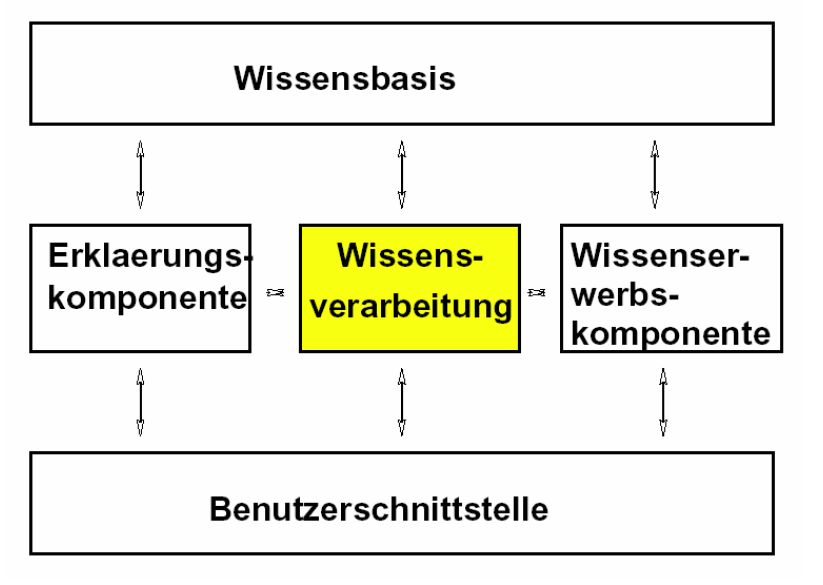
\includegraphics[width=250px]{images/expertensysteme}
\caption{Aufbau eines Expertensystems \cite[s.6]{bib:keller}}
\label{expert_system_structure}
\end{figure}

Die zentrale Komponente ist die \textit{Wissensverarbeitung}. Diese hat auf alle weiteren Komponenten Zugriff und interagiert mit diesen. Es werden die erhaltenen Fakten mithilfe der vorhandenen Regeln verknüpft. Aus der Verknüpfung werden neue Fakten gewonnen, die auf der \textit{Benutzerschnittstelle} angezeigt werden. Die Wissensbasis ist für das Speichern des Expertenwissens in Fakten und Regeln zuständig. Die Speicherung der Daten kann auf folgende zwei Arten geschehen\cite{bib:expert1}:\par
\begin{itemize}
        \item \textbf{generisch}: unabhängig vom aktuellen Anwendungsfall. Meist in einfachen Wenn-Dann-Regeln oder auf einem Modell beruhend. 
        \item \textbf{fallspezifisch}: stellt Lösungen für einen konkreten Anwendungsfall bereit.
\end{itemize}
 Die Pflege dieser Basis erfolgt durch die \textit{Wissenserwerbskomponente}. Mit deren Hilfe lässt sich das vorhandene Expertenwissen in das System einpflegen. Die \textit{Erklärungskomponente} unterstützt das Nachvollziehen des Ergebnisses durch Erläuterungen zu den getätigten Entscheidungen.

\subsection{CAS Configurator Merlin} \label{configurator}
Das Produkt CAS Configurator Merlin ist die Konfigurationslösung der CAS Software AG für große und mittelständische Unternehmen. Das Produkt besteht aus Standardkomponenten, die auf die einzelnen Bedürfnisse der Großkunden angepasst werden. In Abbildung \ref{airbus_structure} ist der Aufbau und das Zusammenspiel der verschiedenen Komponenten des Konfigurators zu sehen: \par
\begin{figure} [H]
\centering
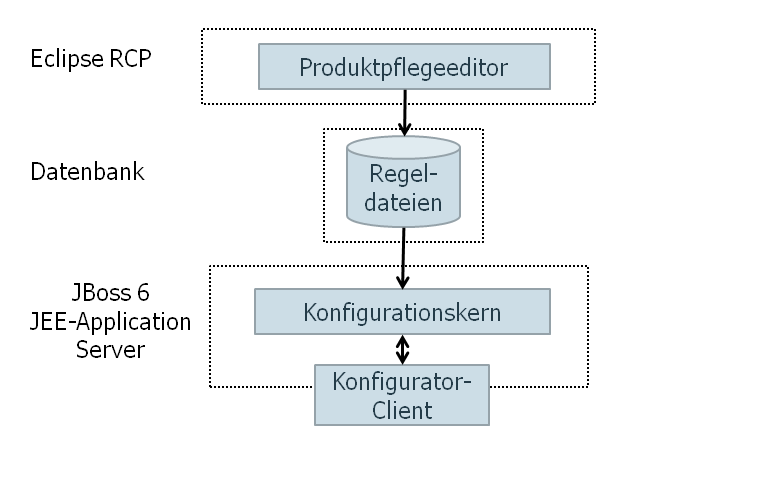
\includegraphics[width=\hsize]{images/AirbusAufbau}
\caption{Architektur und Datenfluss der Merlin Komponenten}
\label{airbus_structure}
\end{figure}
Die Wissensverarbeitungs-Komponente aus Abschnitt \ref{konfiguratoren} ist hier der sogenannte \textit{Konfigurationskern}. Der Kern wertet die zuvor zusammengestellten Produktkomponenten aus. Für die Auswertung verwendet er sogenannte Regeldateien, die mit dem \textit{Produktpflegeeditor} modelliert wurden. Diese Regeln sind auf booleschen Algebra aufgebaut um komplexe Abhängigkeiten der Einzelteile eines Produktes modellieren zu können. Die Speicherung dieser Dateien erfolgt in der \textit{Datenbank}.
\par
 Der Konfigurationskern berechnet ebenfalls sogenannte Alternativen. Diese treten auf, sobald die derzeitige Selektion alleine, ohne Hinzunahme von weiteren Bauteilen, nicht umsetzbar ist. Der Konfigurator kann in diesem Fall neue Möglichkeiten (Alternativen) vorschlagen, damit die Konfiguration durchgeführt werden kann. Die Auswahl der Konfigurationselemente erfolgt im sogenannten \textit{Konfigurator-Client}. Der Client ist mit der Benutzerschnittstelle im Expertensystem zu vergleichen. \par

Der Konfigurationskern, sowie der Client befinden sich auf einem Java-Application-Server. Der Produktpflegeeditor ist eine eigenständige Rich-Client Anwendung, welche auf dem Eclipse Rich-Client-Plattform Framework\cite{bib:eclipseRCP} basiert.

\subsection{Anwendungsbeispiel der Arbeit} \label{airbusConfigurator}
Damit die Arbeit an einem geeigneten Beispiel durchgeführt werden kann, wird der vorhandene Produktkonfigurator eines Flugzeugherstellers verwendet. Hier soll anhand des vorhandenen Prozesses gezeigt werden, wie eine Vereinfachung des gesamten Workflows bei einer Produktkonfiguration mit der Unterstützung einer mobilen Anwendung aussehen kann. \par 
Die aktuelle Konfigurationslösung wird für den Upgradeprozess eines vorhandenen Flugzeuges eingesetzt. Ein Beispiel für ein Upgrade in diesem Bereich können diverse Systemupgrades, wie bspw. ein neues Navigationssystem sein. \par
Dieses Anwendungsfeld ist besonders herausfordern, da somit zu der Auswahl der Produktkomponenten zusätzlich einzelne oder mehrere Flugzeuge ausgewählt werden müssen. Dies hat zur Folge, dass eine übersichtliche Darstellung der Upgrades alleine nicht ausreicht. Es muss ebenfalls eine Lösung für die Auswahl der einzelnen Flugzeuge gefunden werden.  Dadurch, dass jedes Flugzeug individuell zusammengestellt wurde, muss jedes auch eigenständig überprüft werden. 

\subsection{Abgrenzung des Anwendungsbeispiels}



\section{Mobile Anwendungen} \label{mobileAppsGrundlagen}
Die Frage, wie der Kunde besser an dem Entstehungsprozess eines Produktes teilhaben kann und dessen komplexen Aufbau verstehen kann ist nur über ausreichend Kommunikation und Wissensvermittlung zu bewerkstelligen. Eine Möglichkeit zur Unterstützung dieses Prozesses bieten mobile Anwendungen.\par

Diese sind definiert als eine Software, die auf einem Smartphone oder Tablet verwendet wird. Mit dieser Form der Anwendung sind neue Anwendungsgebiete in der Software möglich. Ein neues Einsatzgebiet ist der mobile Einsatz der App bei einem Kunden vor Ort \cite{bib:mobileMarketing}. Hier können insbesondere Tablet-PCs die Kommunikation mit dem Kunden fördern \cite{bib:tableVertrieb}. Die Vorteile durch den großen Bildschirm und die Möglichkeit wie bei einem Blatt Papier den Kunden ins Verkaufsgespräch mit einzubeziehen sind hier überzeugend. Eine Bedienung der Geräte durch Touch-Eingaben ermöglicht eine bessere Interaktion mit der Software. Die Möglichkeiten beim Einsatz dieser Geräte im Geschäftsumfeld ist noch nicht ausgeschöpft und birgt auch weiterhin Potenziale \cite[Fazit]{bib:mobileMarketing2}. In diesem Markt gilt es sich durch gute Anwendungskonzepte zu etablieren. \par

Für Entwickler einer mobilen Anwendung ist der Umgang mit den begrenzten Ressourcen auf dem Endgerät wichtig. 
Aufgrund der geringen Speicherkapazität der mobilen Geräte, sowie die Vermeidung von hohem Synchronisierungsaufwand ist eine Ablegung der Daten auf einem leistungsstärkeren Gerät essentiell. Deshalb ist eine Anbindung an einen Server eine wichtige Grundvoraussetzung bei einer mobilen Anwendung, wenn viele Daten zu verarbeiten sind.  Durch die immer bessere mobile Anbindung an das Internet wird die Verbindung mit einem entfernten System einfacher. Bei der Entwicklung einer mobilen App ist damit die Entscheidung über die Online und Offline Komponenten wichtig.
Ebenfalls von einer großen Bedeutung ist die Auswahl der richtigen Art der Anwendung. Hier stehen drei Möglichkeiten zur Verfügung, die aufgrund von unterschiedlichen Einschränkungen verschiedene Ziele verfolgen. Im Folgenden werden diese drei Arten vorgestellt.

\subsection{Native Anwendungen}
Native Anwendungen sind auf die jeweilige Zielplattform beschränkt \cite{bib:mobilePlattform}. Die Anwendung kann nur auf dem gewählten Betriebssystem ausgeführt werden. Die Programme für native Apps werden dafür mithilfe des vorgegebenen Frameworks entwickelt. Die Verbreitung dieser Anwendungen auf die Endgeräte der einzelnen Benutzer erfolgt über spezielles Software-Stores. Diese Stores werden von den Herstellern der jeweiligen Betriebssysteme bereitgestellt. Die zentrale Verwaltung der Apps sorgt für ein schnelles Verbreiten der Anwendung. \par

 Die Vorteile einer nativen Anwendung liegen im Bereich der Performance und der Funktionen. Da die Programmierung der gegebenen Hardware angepasst wird, sind native Anwendungen für das Zielsystem optimiert. Durch die Optimierung können die Hardwareressourcen besser ausgenutzt werden. Die zweite Stärke von diesem Anwendungstyp ist der erweiterte Funktionsumfang \cite{bib:nativeBS2}. Es können lokale Datenbanken, 3D-Renderer, lokale Sensoren und Ressourcenmanager der Plattform ohne Anpassungen verwendet werden. Dies erhöht die Anzahl der Möglichkeiten, die mit einer nativen Anwendung realisiert werden können. Bei der Verwendung der App in einem Offline Modus(ohne Internetverbindung), kann die native Anwendung ohne Einschränkungen arbeiten. Es ist keine Verbindung mit einem Server notwendig, um Funktionen bereitzustellen. Durch den direkten Speicherzugriff ist eine Speicherung von größeren Onlinedaten ohne größere Probleme möglich. \par
 
 Der Nachteil dieses Anwendungstyp ist, dass die entwickelten Komponenten nicht für andere Plattformen eingesetzt werden können. Bei einer Implementierung für ein anderes Betriebssystem muss die Anwendung neu entwickelt werden. Dies führt zu einem sehr hohen Aufwand bei der Entwicklung. Durch die Vorgabe der Verteilung über die vorhandenen Stores ist man gezwungen die Anwendungen auf diesen bereitzustellen. Hier fallen Kosten für die Qualitätssicherungsmaßnahmen, sowie Gebühren für die Bereitstellung an.

\subsection{Web Anwendungen}
Web Anwendungen sind mobile Webseiten. Diese Seiten wurden mit zusätzlichen Funktionen, die ein mobiles Gerät zur Verfügung hat erweitert und agiert gleich einer App. Der Start der Anwendung erfolgt durch das Aufrufen einer Url im Browser . Es werden dabei die Webtechnologien HTML, CSS und Javascript verwendet. Für die Entwicklung solcher Anwendungen stehen verschiedene Frameworks zur Verfügung. Die Funktionen der web Anwendung werden vom Browser bereitgestellt und hängen von dessen Funktionsumfang ab (Unterstützte HTML-5 Funktionen beliebter Browser: Google Chrome ca. 100, Firefox 93 und Safari 90 Stand: 4.4.2013, Quelle: \cite{bib:webapp}).   \par

Der Hauptvorteil dieses Anwendungstypus liegt bei der plattformübergreifenden Verwendung dieser Apps. Es muss kein bestimmtes Betriebssystem festgelegt werden, für das die Anwendung entwickelt werden soll. Die einzige Voraussetzung zur Verwendung ist ein funktionierender Webbrowser, der bei jedem mobilen Gerät der Standard ist. Der Updateprozess, das Aktualisieren der App, ist ebenfalls sehr einfach, da ein zentraler Server für die Darstellung zuständig ist. Es fallen keine Lizenzgebühren bei der Bereitstellung an, da man den lokalen Store nicht benötigt. 

Der Nachteil liegt am beschränkten Funktionsumfang im Vergleich zu einer nativen App. Da die Webapp für eine möglichst große Zahl an mobilen Geräten verfügbar ist, können nicht alle Funktionen unterstützt werden. Gleichzeitig wird eine weitere Einschränkung durch den Browser hinzugefügt. Von diesem hängt ab, wie viel die Anwendung auf dem Betriebssystem ausführen darf. Dateioperationen beispielsweise sind aus Sicherheitsgründen aus dem Browser heraus nur begrenzt möglich. Die Offline Nutzung der Anwendung ist nur bedingt gegeben. Es kann zwar offline gestartet werden, jedoch stößt man bei einer großen Menge an Daten an Grenzen, da Speicherbeschränkungen für den Browser bestehen.

\subsection{Hybride Anwendung} \label{hybridApplication}
Das Problem der Bereitstellung von mobilen Anwendungen für immer neuere Technologien und Plattformen wird durch den Ansatz einer hybriden App gelöst. Bei dieser Form der Anwendung werden die Vorteile einer nativen und einer web App vereint.  Dieses Ziel wird durch die Verwendung eine Web Anwendung als Kern, der in einen nativen Container eingebunden wird. Der Container ist eine native Anwendung, die den Funktionsumfang der Zielplattform verfügbar macht. Hierbei werden Adapter auf dem Betriebssystem bereitgestellt, die von der Web Anwendung verwendet werden können. Mithilfe des Containers lassen sich mehr native Funktionen verwenden. Dies bietet sich bspw. bei besonders rechenintensiven Operationen an.\par

Die Stärken der hybriden Anwendung liegen in dem erweiterten Funktionsumfang im Gegensatz zu einer Web Anwendung. Durch das Container-Prinzip kann jede Funktion, die bei einer nativen Anwendung verfügbar ist auch verwendet werden. Ebenfalls erfolgt die Verteilung der Anwendung über die jeweiligen Stores, was bei einem schnellen finden der Anwendung hilft. Die Vorteile der hohen Wiederverwendbarkeit der entwickelten Komponenten kommen ebenfalls hinzu. Es ist somit einfacher für mehrere Plattformen eine App zur Verfügung zu stellen. \par

Für die Verwendung auf mehreren Plattformen müssen im Gegensatz zu einer Web Anwendung für jedes Betriebssystem ein neuer Container bereitgestellt werden. Dies erfordert zusätzlichen Aufwand bei der Entwicklung. Hybride Anwendungen kommen durch die zusätzliche Verwendung der Web Technologie nicht an die Performance und Effizienz einer nativen Anwendung heran. 


	\chapter{Analyse der Anwendung}\label{chapter_3}
Damit der Konfigurationsprozess für den Kunden einfacher wird, muss im ersten Schritt der aktuelle Prozess analysiert werden. Darauf aufbauend werden Konzepte zur Vereinfachung dieses Prozesses überlegt und ein neuer Workflow erstellt. Die Anforderungen an die neue Anwendung können mithilfe des neuen Prozesses anschließend spezifiziert werden.

\section{Aktueller Konfigurationsprozess}
Die Anpassungen und Vereinfachungen eines Konfigurationsprozesses bei der Verwendung von mobilen Anwendungen sollen am konkreten Anwendungsbeispiel gezeigt werden. Die Analyse beginnt bei grundlegenden Fragen, wie ein solcher Prozess aufgebaut ist und wird im Folgenden anhand eines konkreten Kundenfalls weiter ausgebaut.

\begin{figure}
\label{oldWorkflow}
\centering
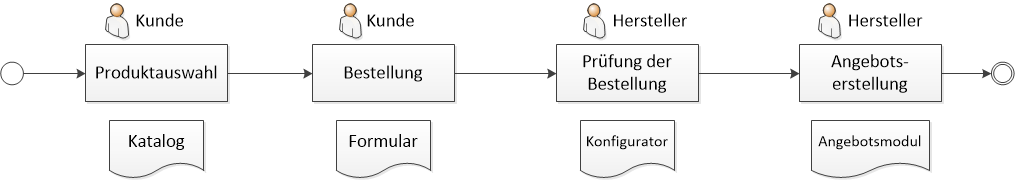
\includegraphics[width=\hsize]{images/konfigurationsprozess_alt}
\caption{Auszug eines Konfigurationsprozesses}
\end{figure}
Ein Auszug aus einem Konfigurationsprozess ist in Abbildung  \ref{oldWorkflow} zu sehen. Die Darstellung zeigt eine Vereinfachung, da in der Praxis auch Schleifen entstehen können. Zu Beginn möchte der Kunde ein konkretes Produkt auswählen. Dieses wird aus dem Katalog herausgesucht.  Anschließend kann er mithilfe von eindeutigen Produktnummern die Bestellung über ein Formular weitergeben. Damit die Zusammenstellung des Kunden geprüft werden kann, werden die Daten beim Hersteller in das Konfigurationssystem eingepflegt. Dieses berechnet die komplexen Abhängigkeiten und prüft die Gültigkeit der Konfiguration. Der letzte Schritt ist die Angebotserstellung. Hierbei wird das konkrete Angebot für den Kunden erstellt.
\par

In der Umsetzung des beschriebenen Prozesses entsteht ein Kommunikationsproblem. Dies tritt aufgrund der Trennung von Produktauswahl und der Prüfung der Bestellung durch den Produktkonfigurator auf. Der Kunde ist nur bei der Auswahl beteiligt. Das Feedback für die Umsetzung der Zusammenstellung erfolgt erst nach der Weitergabe der Bestellung. Probleme zeigen sich, wenn bei der Konfiguration Alternativen auftreten, die vom Kunden zu entscheiden sind, oder eine Konfiguration komplett nicht umsetzbar ist. Hier muss ggf. der Prozess wiederholt werden. Für die Lösung ist eine Hinzunahme des Kunden bei der Konfigurationsüberprüfung notwendig. Das Ziel, welches durch die Erstellung einer mobilen Anwendung erreicht werden soll, ist ein schnelles Feedback bei der aktuellen Auswahl. \par 

Die zweite Stelle, an der eine Verbesserung möglich ist, befindet sich bei der Eingabe der Daten für den Produktkonfigurator und der damit verbundenen Prüfung. Der Kunde hat im vorigen Schritt bereits die Daten für eine Konfiguration erfasst. Eine zweite Erfassung kann zu Fehlern oder Kommunikationsproblemen führen. Diese Probleme entstehen bei der falschen Eingabe des bestellten Produktes. Hierdurch kann der Konfigurator ein falsches Ergebnis liefern, welches zu einem inkorrekten Angebot führt. Auch in einem solchen Fall muss der Prozess wiederholt werden. Für die Verbesserung dieser Situation wird die Auswahl des Kunden direkt an den Konfigurator übermittelt. Diese Maßnahme minimiert die Fehler bei der Erfassung. \par 

Ein weiteres Problem ist die Verwendung von Produktnummern. Diese Nummern dienen einer eindeutigen Identifizierung des Produktes bei der Bestellung. In diesem Schritt kann es passieren, dass der Kunde die falsche Produktnummer auswählt, weshalb nicht das richtige Produkt bei der Angebotserstellung verwendet wird. Bei der Produktauswahl wird dieses Problem umgangen, da die Informationen nicht notwendig sind, der Kunde interessiert sich hierbei nur für das konkrete Produkt. Für die Vereinfachung des Prozesses und eine Fehlerminimierung ist eine automatische Zuordnung der korrekten Nummer im Hintergrund die Lösung. Somit wird der direkte Umgang des Kunden mit einzelnen Produktnummern vermieden und die alleinige Auswahl des Produktes steht für den Kunden im Vordergrund. Hierdurch wird der Kunde nicht mit zu vielen Produktdetails überfordert und es entsteht eine Vereinfachung des Prozesses. \par

Zusammenfassend sind drei grundlegende Probleme beim dargestellten Konfigurationsprozess festgestellt:
\begin{itemize}

		\item zusätzlicher Kommunikationsaufwand durch zu spätes Feedback,
        \item Daten werden doppelt erfasst,
        \item Produktnummern sind für den Kunden schwierig zu handhaben.
\end{itemize}
Diese drei Punkte müssen im neuen Workflow verbessert werden.

\subsection{Übertragung auf die Anwendungsdomäne Luftfahrt}
Beim Anwendungsbeispiel in der Luftfahrt erfolgt die Auswahl der Upgrades ebenfalls über einen Produktkatalog. In diesem Katalog sind die einzelnen Upgrades aufgeführt. Die Auswahl der Produkte erfolgt über eine vorhandene Weboberfläche. Diese Oberfläche ist über die Homepage des Kunden verfügbar. Der Endkunde, im Anwendungsbeispiel eine Fluggesellschaft, wählt das gewünschte Upgrade aus dem Katalog aus. Bei der Bestellung werden die Produktcodes der Auswahl verwendet. Zusätzlich müssen die Flugzeuge angegeben werden, die das Upgrade erhalten sollen. Die Identifizierung erfolgt anhand von eindeutigen Flugzeugcodes. Beide Nummern werden im nächsten Schritt von einem Produktkonfigurator erfasst, der eine Überprüfung der Konfiguration durchführt.   \par 

Beim Kunden wird die klare Trennung der Auswahl und der Überprüfung durch die Verwendung von zwei unterschiedlichen Systemen deutlich. Die Kommunikation der beiden Systeme erfolgt über die Produkt-, bzw. Flugzeugcodes. Bei der Überprüfung der Konfiguration ist der Kunde  nicht involviert. Der Experte bearbeitet die Bestellung und pflegt diese in das System ein. Die Ergebnisse werden anschließend für den Kunden aufbereitet, so dass dieser die auftretenden Alternativen verstehen und entsprechend handeln kann. Diese Besonderheit im Anwendungsbeispiel muss bei der Umstellung des Prozesses beachtet werden. \par 
\begin{figure}[H]
\centering
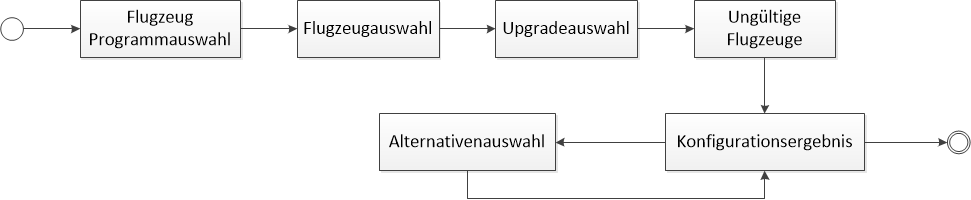
\includegraphics[width=\hsize]{images/workflow_webgui}
\caption{Programmablauf des Anwendungsbeispiels}
\label{webguiAblauf}
\end{figure}

Abbildung \ref{webguiAblauf} zeigt den Ablauf einer Konfiguration mit dem aktuellen System.
Im ersten Schritt wird das passende Flugzeugprogramm ausgewählt. Ein Programm ist eine grobe Einteilung für Flugzeuge nach deren Größe und Art. Die Auswahl ist eine erste Filterung der Datensätze. Des Weiteren werden mit Hilfe des Programms die Regeln ausgewählt, die auf dem Konfigurationsserver für eine Konfiguration verwendet werden. Anschließend folgt die Auswahl der Flugzeuge, die ein Upgrade erhalten sollen. Bei der Identifizierung für eine Bestellung wird die Flugzeugnummer angegeben. Sind die Flugzeuge ausgewählt, werden Upgrades aus einer Liste selektiert. Die Auswahl erfolgt mit der eindeutigen Nummer, welche bei der Bestellung angegeben wird. \par 

Nach dem vorigen Schritt sind alle für die Konfiguration benötigten Elemente ausgewählt. Es folgt eine Validierung der Flugzeuge. Bei dieser Überprüfung werden die einzelnen Flugzeuge auf Konfigurationen untersucht, die in einem Widerspruch mit dem ausgewählten Upgrade stehen. Wenn keine Widersprüche vorhanden sind, werden sogenannte Konfigurationsgruppen gebildet. Eine Konfigurationsgruppe enthält Flugzeuge, die in die gleichen Zielzustände kommen, wenn das Upgrade eingebaut wird. Wenn es mehrere Möglichkeiten gibt, um in einen bestimmten Zustand des Flugzeuges zu kommen, sind sogenannte Alternativen in einer Konfigurationsgruppe enthalten. Damit die Konfiguration vollständig ist, muss der Anwender für jede Gruppe eine Alternative auswählen. \par

Nachdem eine vollständige Konfiguration erzeugt wurde, wird daraus ein Excel-Dokument generiert. In diesem sind die Upgrades enthalten, die in den einzelnen Flugzeugen eingebaut werden müssen. Aus dem Dokument wird ein Upgrade-Angebot erstellt, das anschließend dem Kunden vorgelegt wird. \par 

Das Hauptproblem des aktuellen Systems ist es, dass nur Experten die Anwendung bedienen können. Eine effektive Nutzung kann nur mithilfe der Produktcodes erfolgen. Dies führt dazu, dass man ein großes Wissen über die Produktstruktur besitzen muss. Dadurch kann der Kunde die Konfiguration mit der aktuellen Anwendung nicht selbstständig durchführen. Dieses Problem wird im Folgenden bei der Modellierung des neuen Workflows gelöst.

\section{Workflow Modellierung}\label{workflow_modelling}
Der neue Workflow muss die im vorigen Abschnitt erwähnten Probleme des Konfigurationsprozesses lösen.  Anschließend müssen die Lösungen auf den konkreten Anwendungsfall übertragen werden und ein neuer Programmablauf gefunden werden.

\subsection{Umstellung auf einen mobilen Konfigurationsprozess}\label{mobileConfiguration}
Die Probleme mit der Verwendung von Produktnummern und die doppelte Erfassung der Daten lassen sich durch die Zusammenlegung von Auswahl und Konfigurationsprüfung mit einem System lösen. Diese Maßnahme ermöglicht es dem Kunden die gewünschte Auswahl zu tätigen und gleichzeitig ein Feedback der Konfiguration zu erhalten. Durch die bessere Rückmeldung verringert sich der Kommunikationsaufwand, da der Kunde im Idealfall sofort das Resultat sieht. \par 
 Für eine noch bessere Unterstützung, sowie Hilfestellung beim Aufkommen von Alternativen ist die Durchführung des Prozesses mit einem Mitarbeiter des Herstellers von Vorteil. Dieser kann den Kunden durch die Konfiguration führen oder dabei unterstützen. Gleichzeitig wird hier ein besseres Verständnis für das Produkt ermöglicht. Der Hersteller hat den Vorteil einer Beschleunigung des Prozesses von der Produktauswahl bis zur Angebotserstellung. Er kann durch die direkte Auswahl der Produkte, sowie ein sofortiges Prüfen und ggf. eine Selektion der Alternativen die Konfiguration abschließen und ein  Angebot erstellen. \par 
 
Diese Umstellungen des Prozesses setzt die Verwendung eines mobilen Endgerätes, in diesem Fall eines Tablet-PCs voraus. Durch die Mobilität des Gerätes kann die Konfiguration direkt beim Kunden vor Ort durchgeführt werden. Die verbesserte Kommunikationsmöglichkeit mithilfe des Tablets sorgt für ein besseres Verständnis des Kunden und dessen Wünsche. 


Zusammenfassend sind folgende zwei Maßnahmen beim neuen Workflow durchzuführen: \par

\begin{itemize}
        \item Zusammenlegen von Produktauswahl und Produktkonfiguration. 
        \item Unterstützung durch einen Mitarbeiter des Herstellers.
\end{itemize}
Die konkrete Umsetzung dieser beiden Änderungen wird im Folgenden am Anwendungsbeispiel durchgeführt. \par

\subsection{Soll-Prozess ds Workflows im Anwendungsbeispiels}\label{workflowNew}
Für die Umsetzung der aus Abschnitt \ref{mobileConfiguration} erstellten Maßnahmen müssen die beiden vorhandenen Systeme für die Auswahl und Konfiguration auf ein gemeinsames Gerät portiert werden. Das Konfigurationssystem muss hierfür vereinfacht werden, um den Zugang für den Kunden zu erleichtern. Die Herausforderung besteht hier in einer übersichtlichen Darstellung der Konfigurationsergebnisse. Diese müssen für den Kunden nachvollziehbar aufbereitet werden, weil er nicht die Produktkenntnisse des Experten besitzt. Da der Kunde die Auswahl der einzelnen Produkte "'live"' vornimmt, muss die Anwendung ein schnelleres Feedback erzeugen. Bei der vorherigen Lösung hat der Experte die komplette Zusammenstellung des Kunden erhalten und musste diese in das System übertragen. Beim neuen Workflow dagegen möchte der Kunde die Reihenfolge bei der Auswahl selbst bestimmen. Dies muss im neuen Anwendungsverlauf berücksichtigt werden. \par 
\begin{figure}
\centering
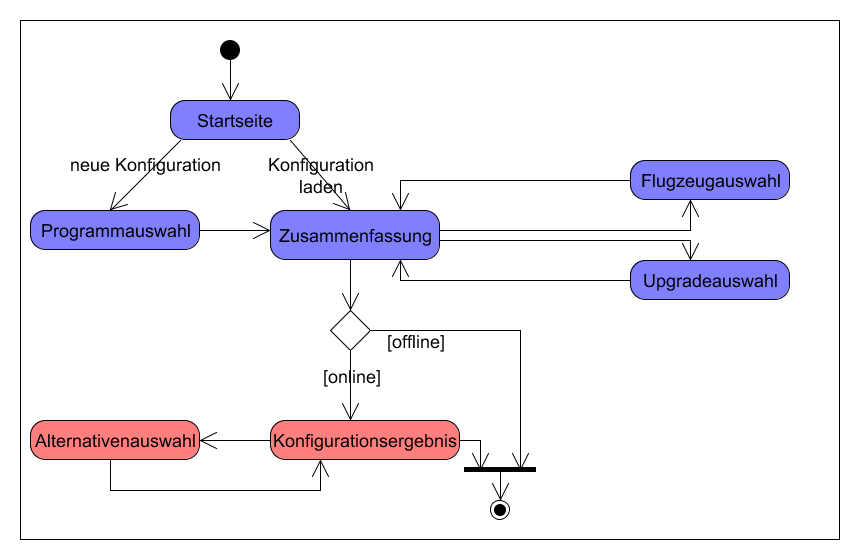
\includegraphics[width=\hsize]{images/workflow_app}
\caption{Workflow der Konfigurator-App}
\label{appWorkflow}
\end{figure}
In Abbildung \ref{appWorkflow} ist der Anwendungsverlauf der App zu sehen, welcher die benannten Problemstellen im Ist-Prozess löst. Analog zu der Weboberfläche wird bei einer neuen Konfiguration zuerst ein Programm (\textbf{Programm-auswahl}) ausgewählt. Dies ist aufgrund einer Filterung der Daten weiterhin notwendig. Nach der Auswahl gelangt der Benutzer in eine \textbf{Zusammenfassung} der aktuellen Konfiguration. Von dieser Ansicht aus können Flugzeuge (\textbf{Flugzeugauswahl}) oder  Upgrades (\textbf{Upgradeauswahl}) selektiert werden. Hier wird den unterschiedlichen Bedürfnissen des Kunden entsprochen und kein strikter Konfigurationsablauf vorgegeben, wie es im vorherigen System war. Mit dieser Umstellung wird dem Kunden die Möglichkeit gegeben die einzelnen Upgrades nacheinander zu wählen und jederzeit eine schnelle Änderung zu ermöglichen. Sobald mindestens ein Flugzeug oder ein Upgrade ausgewählt ist, wird die Konfiguration überprüft. 
Nach der Überprüfung werden die  Konfigurationsgruppen, die der Konfigurator erstellt hat, angezeigt. Diese Gruppen kann der Benutzer einsehen und bei mehreren Alternativen in einer 
separaten Ansicht (\textbf{Alternativenauswahl}) die richtige Lösung auswählen. Ist die Konfiguration vollständig, so hat der Nutzer die Möglichkeit, die aktuelle Zusammenstellung zu bestellen und den Vorgang mit der Bestellung zu beenden. 

Da die Verwendung des Konfigurationsservers, wie in Kapitel \ref{configurator} beschrieben nach dem Client-Server Modell aufgebaut ist, wird eine andere Möglichkeit bei der Konfiguration nötig. Beim mobilen Einsatz der Anwendung kann es passieren, dass eine Verbindung mit dem Konfigurationsserver nicht möglich ist. Aus diesem Grund muss es einen alternativen Weg des Workflows geben. Wenn der Konfigurationsserver nicht verfügbar ist, wird die Konfiguration gespeichert, damit eine Prüfung später durchgeführt werden kann. In diesem Fall ist der Prozesses mit der Speicherung der Konfiguration beendet.

\subsection{Prozessbeteiligte der Anwendung}
Nach der Umstellung des Konfigurationsprozesses müssen die Benutzer der Anwendung identifiziert werden. Dies ist eine Voraussetzung, um die Anforderungen für die Zielgruppe passend zu definieren. Der neue Prozess ist darauf ausgelegt, dass ein Vertreter des Flugzeugherstellers zusammen mit einem Endkunden die Konfiguration durchführt. Der Kunde im Anwendungsbeispiel ist kein unerfahrener Laie. Stattdessen ist er für Upgrades der vorhandenen Flugzeugflotte einer Fluggesellschaft zuständig. Somit ist bereits ein Wissen über das Produkt vorhanden. Dies hat zur Folge, dass der Kunde die Struktur und den Aufbau des Flugzeuges kennt. Dadurch unterscheidet sich die Konfiguration bspw. zu einem Online-Konfigurator eines Autoherstellers. Hier sind unerfahrene Anwender die Zielgruppe, denen der Aufbau des Produktes auf eine andere Weise erklärt werden müsste. \par 
\begin{figure}
\centering
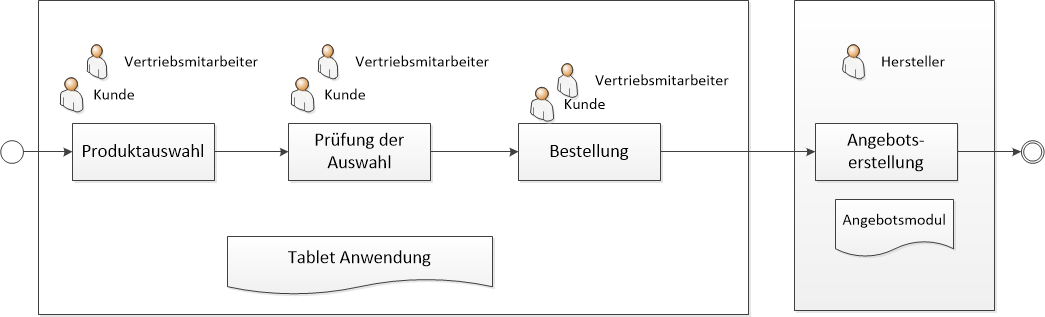
\includegraphics[width=\hsize]{images/konfigurationsprozess_neu}
\caption{Anwendungsbereiche der Tablet Anwendung}
\label{newWorkflow}
\end{figure}
Betrachtet man die Zielgruppe im Workflow des Anwendungsbeispiels,  so stellt man fest, dass
zuvor die Produktauswahl, sowie die Bestellung dem Kunden überlassen wurde. Die neue Tablet Anwendung vereint die einzelnen Prozessschritte, so dass am Ende eine direkte Bestellung folgen kann, die zu einem Angebot führt. Die Durchführung des Konfigurationsprozesses wird im Zusammenwirken von Kunde und Anbieter durchgeführt (siehe Vorgang \ref{newWorkflow}). Dies hat zur Folge, dass die App für zwei unterschiedliche Zielgruppen konzipiert werden muss.


\section{Anforderungsanalyse} \label{requirements}
Nachdem der grundlegende Prozess auf die Bedürfnisse des Kunden, sowie an die mobile Umgebung angepasst ist, können daraus die Anforderungen der Anwendung für das Anwendungsbeispiel festgelegt werden. Bei der Festlegung wird zuerst die allgemeine Anforderung erläutert, sowie anschließend auf das Anwendungsbeispiel spezifiziert. Zur übersichtlichen Darstellung wird im Folgenden zwischen Funktionalen und Nicht-Funktionalen Anforderungen unterschieden. 

\subsection{Nicht-Funktionale Anforderungen}\label{non_functional_requirements}
Die Nicht-Funktionalen Anforderungen betreffen alle Maßnahmen zur Vereinfachung, bzw. Unterstützung des Prozesses, sowie Anforderungen aufgrund des vorhandenen Systems. Diese speziellen Voraussetzungen sind für den Benutzer meistens nicht sichtbar und laufen im Hintergrund, bzw. unbewusst ab. Aus diesem Grund müssen hier auch spezielle Gütekriterien festgelegt werden, um am Ende eine Evaluation zu ermöglichen. Als Basis für diese Anforderungen werden die 10 Heuristiken für Benutzerschnittstellen von Nielsen \cite{bib:heuristicsNielsen} verwendet.
Es lassen sich aus dem neuen Workflow folgende Anforderungen spezifizieren:


\paragraph{Einfache Bedienung:} Der Kunde ist kein Experte und verwendet die Anwendung nicht jeden Tag, somit muss die Bedienung einfach sein. Je weniger bei der Verwendung der Software erklärt werden muss, desto besser ist diese Anforderung erfüllt. Für die Erfüllung dieses Ziels sollen folgende Schwerpunkte der Softwareergonomie \cite{bib:softwareErgonomie} beachtet werden: 
\begin{itemize}
        \item Selbstbeschreibungsfähigkeit
        \item Lernförderlichkeit
        \item Erwartungskonformität
\end{itemize}
Die Kriterien nach Nielsen sind Konsistenz, Erkennung vor Erinnerung und Sichtbarkeit des Systemstatus.

\paragraph{Schnelle Bedienung:} Die zweite Zielgruppe der Anwendung ist der Experte. Für diesen muss es die Möglichkeit einer schnellen Bedienung der Anwendung geben, sodass er möglichst effizient die Konfiguration gestalten kann. Somit wird eine flexible Bedienung der Anwendung nötig. Für eine zusätzliche Steigerung der Effizienz muss die Navigation zwischen den einzelnen Seiten schnell sein. Dies bedeutet, dass beim Übergang von einer zur nächsten Seite der Benutzer nicht lange warten sollte. Ebenfalls muss es genügend Feedback geben, wenn ein Seitenwechsel länger dauern sollte. Hier werden die beiden Heuristiken Sichtbarkeit des aktuellen Status und Flexibilität, sowie Effizienz bei der Benutzung beachtet.

\paragraph{Optimierung auf die Umgebung: } Da ein mobiles Gerät nur begrenzte oder eingeschränkte Resourcen zur Verfügung hat, müssen die einzelnen Bedienelemente auf die Umgebung angepasst sein. Ebenfalls muss die Bedienung für eine Touch-Eingabe optimiert sein. 
Für ein einheitliches Aussehen der Anwendung müssen die Richtlinien der jeweiligen Technologie beachtet werden. Diese Anforderung enthält die beiden Heuristiken ästhetisches und minimalistisches Design, sowie Standards und Konsistenz.

Für eine bessere Übersicht der Nicht-Funktionalen Anforderungen sind diese in der Tabelle \ref{nonFunctionalRequ} dargestellt. Zu jeder Anforderung wird hier ein zusätzlicher Bezeichner definiert.

\begin{table}
\begin{tabular}{| p{0.7cm} | p{2.2cm} | p{4.5cm} | p{5.5cm}|}
\toprule[2pt] \rowcolor{dunkelgrau}
\hline
  Bez. & Anforderung & Beschreibung & Heuristiken nach Nielson \\
  \hline
  N1 & Einfache \newline Bedienung & Die Anwendung soll von unerfahrenen Benutzern bedient werden können.& \begin{itemize}
          \item Sichtbarkeit des aktuellen Status
          \item Erkennung vor Erinnerung
          \item Sichtbarkeit des aktuellen Status
  \end{itemize} \\
  \hline
  N2 & Schnelle \newline Bedienung & Experten müssen die Anwendung schnell und effizient bedienen können. & \begin{itemize}
            \item Flexibilität und Effizienz bei Benutzung
            \item Sichtbarkeit des aktuellen Status
    \end{itemize}  \\
  \hline
    N3 & Optimierung auf Umgebung & Die Anwendung muss auf die Zielplattform optimiert werden. &  \begin{itemize}
              \item Ästhetisches und minimalistisches Design
              \item Standards und Konsistenz
      \end{itemize} \\
    \hline
\bottomrule[2pt]
\end{tabular}
\caption{Nicht-Funktionale Anforderungen mit Bezeichner}
\label{nonFunctionalRequ}
\end{table}

\subsection{Funktionale Anforderungen}\label{functionRequ}
Die Funktionalen Anforderungen sind von der Prozessbeschreibung im Abschnitt \ref{mobileConfiguration} abhängig. Im Folgenden werden diese speziell auf das Anwendungsprojekt spezifiziert. Zusätzlich zu der Spezifikation wird der Bezug zum neuen Workflow hergestellt:

\paragraph{Filterung der Anwendungsdaten: } Da sehr viele Daten vorhanden sind, müssen diese für eine übersichtliche Darstellung im Vorfeld gefiltert werden. Die Filterung erfolgt in zwei Schritten:
\begin{enumerate}
\item Auswahl der Kundendaten: Die Anwendung soll speziell bei einem Kunden eingesetzt werden. Aus diesem Grund kommen nur die kundenspezifischen Daten zum Einsatz.
\item Programmauswahl: Durch die Wahl des Programmes wird eine Filterung der einzelnen Flugzeuge und der möglichen Updates erreicht.
\end{enumerate}
Diese Anforderung wird ebenfalls durch die Verwendung einer mobilen Umgebung notwendig. Damit der zweite modellierte Workflow mit einer nicht vorhandenen Internetverbindung funktioniert, müssen die Daten offline verfügbar sein. Da nur begrenzte Speichermöglichkeiten auf dem Gerät vorhanden sind, können nicht alle Kundendaten gespeichert werden. Dies bedingt eine Filterung durch die Auswahl des Kunden.

\paragraph{Upgradeauswahl: } Bei der Auswahl von Upgrades im Anwendungsbeispiel werden die Funktionen des Produktkataloges benötigt. Es muss möglich sein, ein bestimmtes Produkt an- oder abzuwählen. Damit der Kunde den Aufbau des Produktes versteht, müssen die einzelnen Produkte nach einer bestimmten Struktur geordnet sein. 

\paragraph{Flugzeugauswahl: } Flugzeuge, die ein ausgewähltes Upgrade erhalten sollen, müssen ebenfalls in der Anwendung auswählbar sein. Die Anforderungen an diese Auswahl sind nicht die Gleichen wie bei der Produktauswahl. Der Schwerpunkt muss hier auf ein schnelles Finden der einzelnen Flugzeuge gelegt werden. Dies wird ebenfalls durch eine dem Kunden bekannte Struktur erreicht. 

\paragraph{Anzeige der Konfigurationsergebnisse: } Damit der Kunde ein schnelles Feedback der aktuellen Auswahl erhält, müssen die Konfigurationsergebnisse angezeigt werden. Dies impliziert eine Anbindung an den Konfigurationsserver, der die entsprechenden Ergebnisse berechnet. Diese Anzeige muss eine vereinfachte Darstellung beinhalten, damit der Kunde diese Ergebnisse verstehen kann.

\paragraph{Alternativenauswahl: } Damit eine vollständige Konfiguration erzeugt werden kann, muss die Anwendung eine Auswahl für Alternativen bereitstellen. Hierbei muss das Verständnis des Kunden für das Produkt berücksichtigt werden. Die Alternativen müssen auf eine verständliche Art dargestellt sein. 

\paragraph{Speichern und Laden der Konfiguration: } Die zweite Voraussetzung des alternativen Offline Workflows ist eine Speicherung der Konfiguration. Für eine spätere Bearbeitung ist das erneute Laden der Konfiguration notwendig. Diese beide Anforderungen werden aufgrund der mobilen Zielumgebung benötigt.

Die Zuordnung der einzelnen Anforderungen zu den jeweiligen Prozessschritten ist in Tabelle \ref{functionalRequirements} zu sehen. Hierbei werden die drei Prozessanforderungen Produktkatalog, Konfiguration und mobile Zielumgebung unterschieden.
\par 
\begin{table}

\begin{tabular}[H]{| p{0.4cm} | p{2.5cm} | p{5.9cm} | p{4.5cm} |}
\toprule[2pt] \rowcolor{dunkelgrau}
\hline
  NR. & Anforderung & Beschreibung & Prozesszuordnung \\
  \hline
  F1 & Upgrade-auswahl & Es sollen Upgrades für Flugzeuge auswählbar sein & Produktkatalog
   \\
  \hline
  F2 & Flugzeug-auswahl & Es müssen Flugzeuge eines bestimmten Kunden auswählbar sein. & Produktkatalog  \\
  \hline
    F3 & Konfigurations-ergebnisse anzeigen & Übersichtliche Darstellung der aktuellen Zusammenstellung & Konfiguration \\
    \hline
     F4 & Alternativen-auswahl & Bei mehreren Möglichkeiten einer Auswahl sollen Alternativen ausgewählt werden können & Konfiguration \\
        \hline
    F5 & Speichern und Laden & Die getätigte Auswahl soll gespeichert und geladen werden können& mobile Zielumgebung \\
    \hline
    F6 & Filterung der Anwendungsdaten & Die Daten (Flugzeuge und Upgrades) müssen gefiltert werden können & mobile Zielumgebung \\
    \hline
\bottomrule[2pt]
\end{tabular}
\caption{Funktionale Anforderungen mit Bezeichner}
\label{functionalRequirements}
\end{table}






	\chapter{Entwurf der Benutzerschnittstelle}\label{chapter_4}
Die Anforderungen der Anwendung für die Unterstützung des neuen Workflows wurden im vorigen Kapitel spezifiziert. Diese Kriterien werden im nächsten Schritt in einem Entwurf der Benutzerschnittstelle umgesetzt. Bevor die Schnittstelle entworfen werden kann, muss die geeignete Anwendungsform und eine darauf basierende Technologie ausgewählt werden. Anschließend folgt eine kurze Analyse der Zielplattform und deren Konzepte, damit diese beim Entwurf berücksichtigt werden können.

\section{Auswahl der Anwendungsplattform}
Aufgrund der vielen Möglichkeiten bei der Entwicklung von mobilen Anwendungen muss die Anwendungsart und Technologie richtig gewählt werden. Hierbei soll zuerst die passende Anwendungsform (Nativ, Web oder Hybrid siehe \ref{mobileAppsGrundlagen}) gewählt werden. Durch diese Vorauswahl, wird die Anzahl der möglichen Technologien begrenzt, was im folgenden Schritt die Auswahl vereinfacht.


\subsection{Anwendungsform}
Damit die richtige Anwendungsform der App ausgewählt werden kann, müssen die drei Möglichkeiten Nativ, Web und Hybrid auf ihre Eignung bei der Umsetzung der Anforderungen untersucht werden. Für eine Entscheidungsgrundlage werden konkrete Kriterien festgelegt. 
Die Umsetzung der rein fachlichen Funktionen Produktauswahl und Konfiguration kann mit jeder Anwendungsform durchgeführt werden. Hier sind die Unterschiede für eine Auswahl nicht ausreichend. \par

Bei den  funktionalen Anforderungen sind die zwei Kriterien, die aufgrund der mobilen Zielumgebung wichtig sind für die Auswahl bedeutend. Diese sind das Speichern und Laden (F5), sowie die Filterung der Anwendungsdaten (F6). Für die Umsetzung dieser Funktionen ist eine Verwendung des Dateisystems auf der mobilen Zielumgebung notwendig. Hier muss eine Form der Speicherung, ob Datenbank oder einfaches Speichern in einer Datei möglich sein. Diese Voraussetzung ist für die Entscheidung der Anwendungsform essentiell. \par

Das zweite Kriterium leitet sich von den nicht-funktionalen Anforderungen einer schnellen Bedienung (N2) ab. Damit die Anwendung schnell bedient werden kann, müssen die vorhandenen Hardwareressourcen optimal verwendet werden können. Dies ist notwendig, um bspw. das Laden von Bildern zu beschleunigen. Ebenfalls müssen Seitenübergänge ohne große Wartezeiten möglich sein, um die Anforderung erfüllen zu können. Die Anwendungsform muss für die Umsetzung Schnittstellen bereitstellen, die auf die vorhandene Hardware optimiert sind.

Für eine Optimierung der Anwendung auf die Zielumgebung (N3) ist ein ästhetisches und minimalistisches Design die entscheidende Heuristik für die Auswahl der Anwendungsform. Für die Implementierung muss eine gute optische Integration in das System vorhanden sein. Dies ist für eine übersichtliche Aufbereitung des Produktkataloges eine Voraussetzung. Der App-Typ muss Oberflächenelemente zur Verfügung stellen, die zu der Gesamtumgebung passen. Durch eine gute Integration in die Zielumgebung wird dadurch die Anwendung ästhetischer. Die gesamte Wahrnehmung der App wird hierdurch verbessert. Das dritte Zielkriterium für die Auswahl ist somit die Verwendung von betriebssystemspezifischen Oberflächenelementen.    

Im Folgenden werden die drei festgestellten Kriterien lokale Speicherung der Daten, Hardwarenahe Schnittstellen und Verwendung von betriebssystemspezifischen Oberflächenelementen  für jede Anwendungsform bewertet, sodass am Ende eine Gegenüberstellung stattfinden kann.

\paragraph{Native Anwendung: }Bei Nativen Anwendungen ist der komplette Funktionsumfang der mobilen Zielplattform verfügbar. Dies ermöglicht ein breites Anwendungsfeld für native Anwendungen.
\begin{itemize}
\item \textbf{Lokale Speicherung der Daten:} Die native Anwendungsform stellt Schnittstellen für den Zugriff auf eine lokale Datenbank oder ein lokales Dateisystem bereit. Diese können ohne Anpassungen verwendet werden.

\item \textbf{Hardwarenahe Schnittstellen:} Dadurch, dass die einzelnen Schnittstellen direkt vom Hersteller der jeweiligen Plattform bereitgestellt werden, sind die Operationen für das jeweilige System optimiert. Mit einer nativen Anwendung wird damit die beste Performanz erreicht. 

\item \textbf{Betriebssystemspezfische Oberflächenelemente:} Native Anwendungen verwenden für die Benutzerschnittstelle die nativen Oberflächenelemente. Weiterhin werden spezielle Elemente bereitgestellt, die für eine Verwendung mit Touchscreen optimiert sind. 
\end{itemize}

Auf die einzelnen Kriterien bezogen erfüllt die native Anwendung alle Anforderungen ohne Einschränkungen. Der volle Funktionsumfang des Systems ist gegeben, wodurch die App ideal an die gewählte Zielplattform angepasst werden kann.

\paragraph{Web Anwendung: } Web Anwendungen werden im Browser ausgeführt. 
 Dies führt dazu, dass nur Funktionen verwendet werden können, die der jeweilige Browser auf der Zielplattform zur Verfügung stellt. 
 \begin{itemize}
 \item \textbf{Lokale Speicherung der Daten:} Ein Speichern und Laden der Daten vom Betriebssystem ist bei einer Web Anwendung nicht ohne weiteres möglich. Der Browser verbietet durch ein Sandbox-Modell einen direkten Zugriff auf das System.  Ein Ansatz zur Lösung des Problems ist die Installation des Servers direkt auf dem Zielsystem, so dass dieser lokal zur Verfügung steht. Eine Erfüllung der Anforderungen ist damit möglich, jedoch mit erheblichem Mehraufwand. 
 
 \item \textbf{Hardwarenahe Schnittstellen:} Die Kommunikation mit dem Betriebssystem erfolgt durch den Browser. Diese zusätzliche Zwischenschicht sorgt dafür, dass die Hardware nicht direkt verwendet wird, wie es bei einer nativen Anwendung der Fall ist. Der zusätzliche Overhead sorgt dafür, dass die Performance bei einer Web Anwendung nicht ideal im Vergleich zur nativen Lösung ist.
 
 \item \textbf{Betriebssystemspezfische Oberflächenelemente:} Die grundlegenden Oberflächenelemente sind HTML Elemente. Diese können mit Javascript und CSS einen passenden Stil für das jeweilige Betriebssystem erhalten. Die Verwendung von speziellen Touch Gesten ist mit Web Anwendungen aufgrund der Interoperabilität mit mehreren Betriebssystemen schwieriger. Hier sind ebenfalls nur begrenzte Interaktionen möglich.
 
 \end{itemize}
 Der Hauptvorteil der Web Anwendung die Verwendung auf mehreren Systemen ohne eine komplett neue Implementierung ist aufgrund der Kriterien des Anwendungsbeispiels nicht relevant. Die wichtigen Eigenschaften der Anwendung Performanz und lokale Speicherung können mit dieser Anwendungsform gelöst werden, jedoch mit einem deutlichen Mehraufwand und Einbußen bei der Performanz.


\paragraph{Hybride Anwendung: }Durch die Verwendung der lokalen Schnittstellen im nativen Anwendungscontainer (siehe \ref{hybridApplication}) können die vorhanden Ressourcen wie bei einer Nativen Anwendung verwendet werden. Dies führt zu einigen Verbesserungen gegenüber einer reinen Web Anwendung.

\begin{itemize}
 \item \textbf{Lokale Speicherung der Daten:} Für die Umsetzung dieser Anforderung muss eine geeignete Schnittstelle im Anwendungscontainer zur Verfügung gestellt werden. Hierdurch wird eine Verwendung des Dateisystems möglich. Das Kriterium kann ohne Einschränkungen erfüllt werden. 
 
 \item \textbf{Hardwarenahe Schnittstellen:} Durch den Anwendungscontainer wird, wie bei einer Webanwendung der Browser, eine Zwischenschicht nötig. Dadurch entsteht ein zusätzlicher Kommunikationsaufwand. Dieser zusätzliche Aufwand verringert die Performanz der Anwendung.
 
 \item \textbf{Betriebssystemspezfische Oberflächenelemente:} Die Oberflächenelemente des Betriebssystems lassen sich im Container bereitstellen. Somit können die nativen Elemente in der Hybriden Anwendung verwendet werden. Die Verwendung der Touch Bedienelemente eine Plattform wird durch dieses Konzept ermöglicht.
 \end{itemize}
 Die Probleme, die bei der Verwendung einer Web Anwendung auftreten können durch den hybriden Ansatz gelöst werden. Ein Problem was weiterhin besteht, ist die Performanz. Diese wird mit der hybriden Anwendungsform besser, kommt jedoch nicht an die Leistung einer nativen Anwendung heran.

\paragraph{Abwägung: }

Nachdem alle Anwendungsformen auf die Erfüllung der aufgestellten Kriterien untersucht sind, kann eine Gegenüberstellung der einzelnen Komponenten erfolgen. Die Tabelle \ref{decision} zeigt eine Bewertung der Kriterien. Hierbei wurden die einzelnen Punkte anhand einer Skala von 0 (kann nicht erfüllt werden) bis 5 (ohne Einschränkungen möglich) bewertet.  Die Implementierung als Web Anwendung scheidet klar aus. Jede Anforderung kann zwar umgesetzt werden, jedoch ist ein erheblicher Mehraufwand bei der Implementierung notwendig. Aus diesem Grund wird jeweils nur ein Punkt vergeben. Weiterhin hat die Anwendung im Vorhinein bereits Einschränkungen bzgl. der Performanz, sowie der Bereitstellung von Oberflächenelementen. Die Vorteile einer Verfügbarkeit der Anwendung für mehrere Zielsysteme mit einer Implementierung ist bei der Umsetzung kein Kriterium. \par
\begin{table}
\begin{tabular}{| p{5.4cm} | p{2.5cm} | p{2.5cm} | p{2.5cm} |}
\toprule[2pt] \rowcolor{dunkelgrau}
\hline
  Kriterium & Web \newline Anwendung & Hybride \newline Anwendung & Native \newline Anwendung \\
  \hline
  Lokale Datenspeicherung & 1 & 4 & 5
   \\
  \hline
  Hardwarenahe Schnittstellen &1  &2  & 5  \\
  \hline
    Betriebssystemspezifische Oberflächenelemente & 1 & 4 & 5 \\
  \hline
    Summe & 3 & 10 & 15 \\
  \hline
\bottomrule[2pt]
\end{tabular}
\caption{Gegenüberstellung und Bewertung der Zielkriterien für die Anwendungsform}
\label{decision}
\end{table}
\par 
Schwieriger ist die Entscheidung zwischen dem hybriden und nativen Ansatz. Die beiden Kriterien lokale Speicherung der Daten und betriebssystemspezifsche Oberflächenelemente sind mit beiden Ansätzen ohne größere Einschränkungen möglich. Beim hybriden Ansatz ist ein geringer Mehraufwand bei der Implementierung nötig, deshalb wird hier nicht die volle Punktzahl gegeben. Dies ist jedoch nicht relevant für die Entscheidung. Der wichtigste Grund für die Entscheidung für eine nativen Anwendung ist die Performanz bei der Bedienung. Nur durch die Verwendung von nativen Anwendungen können aufwändige Animationen oder das Rendern von vielen Bildern flüssig ablaufen. Eine hybride Lösung besitzt hier Einschränkungen, da die Hardware mit einer Zwischenschicht verwendet wird, deshalb die Bewertung mit zwei Punkten. Weiterhin können die Touch Bedienelemente der Zielplattform bei einer nativen Anwendung besser verwendet werden, da keine Kompromisse notwendig sind.

\subsection{Anwendungstechnologie}
Mit der Entscheidung für eine mobile Anwendungsform kommen drei mögliche Technologien für die Implementierung in Frage. Die Plattformen Android \footnote{http://www.android.com/}, iOS \footnote{http://www.apple.com/de/iphone/ios/} und Windows 8 \footnote{http://windows.microsoft.com/de-de/windows-8/} sind aufgrund ihrer Marktanteile (Android: 43,4\% iOS: 48,2\% Windows: 7,4\% Quelle: \cite{bib:marktanteilBS} ) die wichtigsten Technologien im Tablet Bereich. Die drei Plattformen haben unterschiedliche Ziele. Das iOS Betriebssystem hat den Vorteil einer hohen Verbreitung bei Business Anwendungen (siehe \cite[S.5]{bib:mobileMarketing2}). Android hat die meisten Nutzer bei Privatanwendungen (siehe \cite{bib:marktanteilMBS}). Bei Windows 8 ist der Vorteil eines neuen Konzeptes, was speziell für Tablet-PCs optimiert ist. Für die Umsetzung des Workflows kann jede dieser Technologien verwendet werden, da die Zielkriterien sich bei den unterschiedlichen Plattformen nicht unterscheiden (siehe Tabelle \ref{decisionTechnologie}). Einziger Abzug erhält Android bei der Performanz, da eine Java-Virtual-Machine verwendet wird, die im Vergleich zu den C, bzw. C++ Schnittstellen der anderen beiden langsamer ist. Ist die Implementierung mit einem Framework umgesetzt, stellt die Übertragung auf einer anderen Zielplattform keine Herausforderung dar. \par 
\begin{table}
\begin{tabular}[H]{| p{5.4cm} | p{2.5cm} | p{2.5cm} | p{2.5cm} |}
\toprule[2pt] \rowcolor{dunkelgrau}
\hline
  Kriterium & Android & iOS & Windows 8 \\
  \hline
  Lokale Datenspeicherung & 5 & 5 & 5
   \\
  \hline
  Hardwarenahe Schnittstellen &4  &5  & 5  \\
  \hline
    Betriebssystemspezifische Oberflächenelemente & 5 & 5 & 5 \\
  \hline
    Summe & 14 & 15 & 15 \\
  \hline
\bottomrule[2pt]
\end{tabular}
\caption{Gegenüberstellung und Bewertung der Zielkriterien für Plattform}
\label{decisionTechnologie}
\end{table}

Bei der vorliegenden Arbeit wird auf Windows 8 gesetzt. Im Gegensatz zu iOS und Android wird dieses Betriebssystem nicht auf Smartphones ausgeführt. Dies führt zu einer besseren Optimierung für größere Bildschirme. Die Technologie ist sehr neu auf dem Markt (26. Oktober 2012), dadurch gibt es noch nicht viele Apps. Dies bietet die Möglichkeit den Anwender mit neuen Möglichkeiten in der Anwendung zu überraschen, da einige Konzepte noch nicht bekannt sind. Die Möglichkeit zu experimentieren und neue Ideen umzusetzen ist aufgrund der neuen Plattform vorhanden.  Die Verwendung von Windows 8 vereinfacht ebenfalls die Integration in ein Unternehmensumfeld, da hier die Microsoft Produkte weit verbreitet sind. Dies führt zu einer schnelleren Akzeptanz im Unternehmen. Somit wird im Folgenden die Anwendung für das Windows 8 Betriebssystem implementiert.
        

\section{Untersuchung der Plattform Windows 8}
Damit die Anforderung eines ästhetischen und minimalistischen Designs (N3) erfüllt ist, muss vor der Gestaltung der einzelnen Ansichten die Zielplattform untersucht werden. Die Designgrundlagen müssen verstanden werden, um ein passendes Aussehen realisieren zu können. 
Die Folgende Untersuchung wird in drei Teile aufgeteilt. Im ersten Abschnitt werden allgemeine Design Prinzipien behandelt, darauf aufbauend die Bedienkonzepte und touchoptimierten Bedienelemente der Plattform.

\subsection{Design Richtlinien}
Damit einheitliche Apps entwickelt werden, hat Microsoft Richtlinien (Entnommen aus: \cite{bib:win80}, \cite{bib:win81}, \cite{bib:win82}, \cite{bib:win83}) aufgestellt. \par
\begin{figure}[H]
\centering
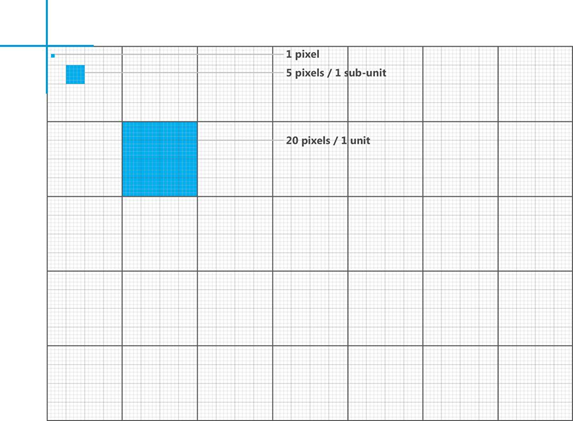
\includegraphics[width=300px]{images/grid}
\caption{Grid mit eingezeichneten Kacheln (Quelle: \cite{bib:gridTile}, Microsoft)}
\label{gridAndTile}
\end{figure}
Das wichtigste Design Element bei einer Windows 8 Anwendung sind sogenannte Kacheln (siehe blaues Quadrat in Abbildung \ref{gridAndTile}). Diese Kacheln sind quadratisch und in jeder App vorhanden. Jede Funktion wird über eine Kachel erreicht. Sie soll mehr Informationen enthalten, als ein einfaches Logo oder Icon auf einem Button. Durch einen dynamischen Inhalt und unterschiedliche Größen wird dem Benutzer ein neues Benutzererlebnis gegeben. Die Organisation der Kacheln erfolgt in einem sogenannten Grid (engl. für Gitter). Dieses besteht aus mehreren Quadraten, wie in Abbildung \ref{gridAndTile} zu sehen. Das kleinste Quadrat hat eine Größe von einem Pixel. Das Grid besitzt verschiedene Bereiche für die Überschrift und den Inhalt. Dieser ist vorgegeben und sollte eingehalten werden. \par 

Die Anwendung muss sich auf die Anzeige des Wesentlichen konzentrieren. Microsoft nennt  das Prinzip "'Content over Chrome"'.  Für die Umsetzung dieser Richtlinie soll die Anwendung nur die wichtigsten Funktionen in der Ansicht darstellen. Es sollen überladene Ansichten vermieden werden und stattdessen bewusst größere Elemente mit mehr Platz verwendet werden. 
 
Ein weiteres wichtiges Design Element ist die Typographie. Hier geht es um die bewusste Gestaltung von Schriften. Die Kalligrafie wird als Vorbild verwendet.  Die Idee ist keine rein statische Verwendung der Texte. Der Nutzer soll die Möglichkeit haben diese auszuwählen, damit eine Interaktion ermöglicht wird. 

Die erläuterten Richtlinien werden beim Entwurf der einzelnen Ansichten berücksichtigt. 


\subsection{Bedienkonzepte}\label{usingConcepts}
Bei den Konzepten für die Bedienung steht bei Windows 8 eine besondere Optimierung für Tablet-PCs im Vordergrund. Es werden deshalb sehr viele Gesten verwendet. Eine wichtige Geste ist das sogenannte "'wischen"'. Diese Aktion ist von jeder Seite des Bildschirms erlaubt. Beim Wischen von oben oder unten wird die sogenannte AppBar eingeblendet. Diese Bar wird an der oberen Seite für die Navigation durch die Anwendung verwendet. Dies ermöglicht einen schnellen Wechsel zwischen den Ansichten. Die untere AppBar wird für Aktionen verwendet, die nicht Vordergrund stehen. Ein Beispiel wäre die Filterung der Eingabedaten nach bestimmten Kriterien. Ein Wischen von der rechten Seit lässt die sogenannte CharmBar erscheinen. Der Inhalt dieser Bar ist die Verwendung von sogenannten Contracts (engl. Verträge). Diese Funktionen werden für alle Anwendungen durch das Betriebssystem bereitgestellt. An dieser Stelle können Einstellungen oder Suchen durchgeführt werden. \par 

Das zweite wichtige Bedienkonzept ist das horizontale Scrollen. Aufgrund der größeren Bedienelemente sind nicht immer alle Elemente sichtbar. Die Lösung ist ein horizontales Ausbreiten des Inhalts. Damit die Inhalte verwendet werden können, wird ein horizontales Scrollen mit einer Wisch-Geste durchgeführt. Hier muss darauf geachtet werden, dass ein Ausschnitt des nächsten Elementes sichtbar ist, damit dem Benutzer die Erweiterung der Ansicht signalisiert wird. \par 

Beim Aufbau der Anwendung kann entweder eine hierarchische (Baumstruktur) oder  flache (linear) Struktur verwendet werden. Für den in Abschnitt \ref{workflowNew} erstellen Workflow ist eine hierarchische Architektur passender, da kein linearer Verlauf bei der Verwendung entsteht. Der Ursprung geht hierbei immer von der Startseite, der sogenannten Hub-Page aus. Diese Seite ist der zentrale Startpunkt, von der alle weiteren Aktionen ausgehen. Auf der zweiten Ebene befinden sich sogenannte Section Pages. Diese stellen den Inhalt einer  Kategorie dar. Die unterste Ebene sind die Detail Pages. Diese enthalten die jeweiligen Details eines Elementes in einer Kategorie. Bei einer Zeitungs App wären beispielsweise auf der Startseite die einzelnen Kategorien wie Politik, Wirtschaft oder Sport zu sehen. In der Kategorie Ansicht die jeweiligen Überschriften der Artikel. Die Detail Seite würde den Artikel anzeigen. Dieser baumartige Aufbau wird durch das Verwenden eines Zurück Buttons unterstützt, der in jeder Ansicht, außer der Startseite vorhanden ist. Durch diesen Button wird dem Benutzer eine weitere Navigationsmöglichkeit gegeben.

Beim Design der Ansichten ist ein durchdachtes Bedienkonzept aufgrund der beiden Anforderungen N1 und N2 (einfache und schnelle Bedienung) wichtig. Die Möglichkeiten, die zur Verfügung gestellt werden, sollten beim ersten Entwurf der App enthalten sein.

\subsection{Touchoptimierte Bedienelemente}
Für die Unterstützung der Bedienung durch Gesten enthält das Framework besondere Oberflächenelemente. Diese sind für die Verwendung mittels Touch optimiert. Die in der Arbeit verwendeten Elemente werden im Folgenden vorgestellt.
Die Design Richtlinien von Microsoft erzeugen Probleme bei der Darstellung von vielen Daten. Eine Umsetzung der Richtlinie "'Content over Chrome"', sowie die Darstellung auf einem Gerät mit kleinerem Bildschirm verursachen einen großen Aufwand beim Scrollen. Hierdurch kann es sein, dass eine lange Zeit für das Auswählen eines bestimmten Datums benötigt wird. \par


Für die Lösung dieses Problems bietet Windows 8 den sogenannten semantischen Zoom an. Diese Funktion wird mit einer Kneif-Geste, welche sich als allgemeine Geste für das Zoomen etabliert hat, auf dem aktuellen Datensatz durchgeführt. Hierdurch wird die Ansicht nicht optisch verkleinert. Es erfolgt ein Wechsel von der Detailansicht zu einer Kategorieansicht. Die Datensätze werden somit semantisch verkleinert, wodurch ein schnelles Navigieren zum gewünschten Datum möglich ist. \par 
\begin{figure}
\centering
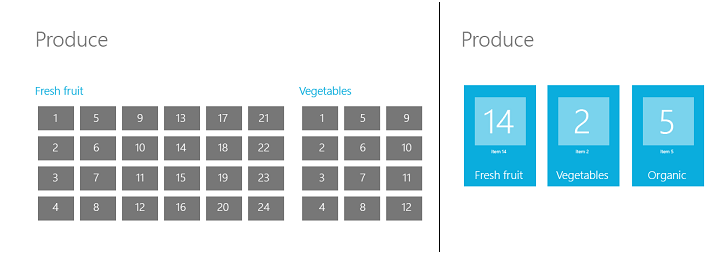
\includegraphics[width=\hsize]{images/semanticZoomOut}
\caption{Semantischer Zoom in zwei Ansichten (Quelle: \cite{bib:semanticZoom}, Microsoft)}
\label{semanticZoomIllustration}
\end{figure}
Ein Beispiel ist in Abbildung \ref{semanticZoomIllustration} zu sehen. Hier sind in der linken Ansicht alle Elemente (Produkte) in der jeweiligen Kategorie vorhanden. Nach dem Anwenden der Kneif-Geste gelangt man zu einer zusammengefassten Ansicht (rechtes Bild), in der nur die Kategorien mit der Anzahl der vorhandenen Elemente sichtbar sind. \par 

 Der Semantische Zoom darf nicht geschachtelt verwendet werden und ist damit auf eine Ebene beschränkt. Voraussetzung für die Verwendung des Zooms ist die Einteilung der Daten in Kategorien. Ohne diese Kategorien kann keine übergeordnete Ansicht erstellt werden.

Das zweite neue Bedienelement, welches für eine Touch-Optimierung dient, ist die sogenannte Flip-View. Mit ihr kann durch ein Wischen von der linken oder rechten Seite die Ansicht gewechselt werden. Dieses Element kann den Benutzer bei einem schnellen navigieren helfen. Es sollten jedoch nicht zu viele Elemente für einen Wechsel enthalten.

\section{Entwurf der Ansichten}
Die vorgestellten Konzepte der Anwendungsplattform, sowie die einzelnen Bedienelemente werden für den Entwurf der Ansichten verwendet. Der Workflow der App, wie in Abschnitt \ref{appWorkflow} beschrieben, wird hier als Grundlage verwendet. Damit alle Prozessschritte durchgeführt werden können, muss für jeden Zustand eine Ansicht vorhanden sein. Außerdem werden für die Umsetzung der Anforderungen aus Kapitel \ref{functionalRequirements} evtl. zusätzliche Benutzerschnittstellen benötigt.


\subsection{Hauptfunktion der Anwendung}
Um den Benutzer bei der Verwendung der App zu unterstützen, müssen zu Beginn die Hauptfunktionen der Anwendung erkennbar gemacht werden. Diese Funktionen sollen gut platziert werden, um eine schnelle Bedienung zu ermöglichen. Die Platzierung erfolgt in der Hauptansicht, von der alle weiteren Aktion ausgehen.

Bei der vorliegenden Arbeit sind die Hauptfunktionen der Produktkatalog und die Konfiguration. Im Anwendungsbeispiel ist die Auswahl der Flugzuge eine Voraussetzung für eine vollständige Konfiguration. Aus diesem Grund gehört die Flugzeugauswahl ebenfalls zu den Hauptfunktionen. Wie im neuen Workflow modelliert, sind diese drei Funktionen von der Zusammenfassungsseite aus zugänglich. Somit ist diese Seite die Hauptfunktionsseite\par 
\begin{figure}[H]
\centering
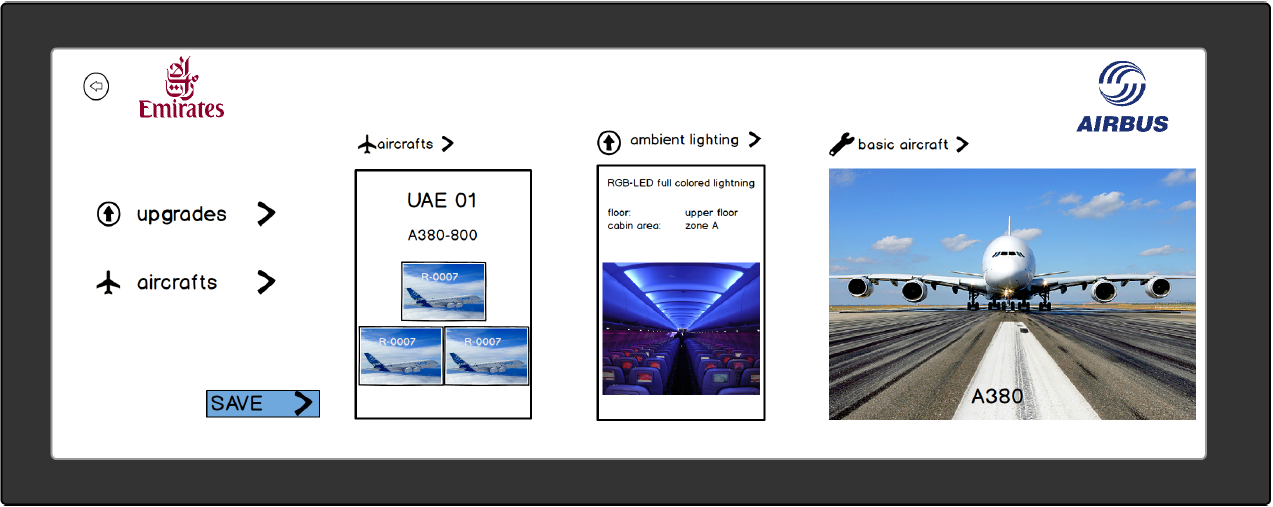
\includegraphics[width=\hsize]{images/summary_entwurf}
\caption{Entwurf der Zusammenfassung Seite}
\label{summarySketch}
\end{figure}

Der erste Entwurf der Zusammenfassung ist in Abbildung \ref{summarySketch} zu sehen. Die Hauptfunktionen Upgradeauswahl und Flugzeugauswahl sind als Buttons mit Text und Icon auf der linken Seite zu sehen. Bei der Selektion eines Buttons wird die jeweilige Ansicht der Auswahl geöffnet. Die weiteren Elemente der Zusammenfassung bestehen aus der aktuellen Auswahl. Die Darstellung erfolgt immer mit einem Bild und dem passenden Text in der Kachel Optik. Auf der ganz rechten Seite wird zuerst das ausgewählte Flugzeugprogramm angezeigt. Daneben werden die bisher ausgewählten Upgrades und Flugzeuge dargestellt. Die Reihenfolge der Darstellung hängt von der Auswahl ab. Diese werden in der gleichen Abfolge wie diese zuvor ausgewählt wurden angezeigt. Damit wird das zuletzt Gewählte immer auf der linken Seite angezeigt. Bei der Zusammenfassungsseite werden die Microsoft Richtlinien für das horizontale Scrollen umgesetzt. Die einzelnen Elemente sind im Grid angeordnet.


\subsection{Produktkatalog}
Für das Verwenden der ersten Hauptfunktion, der Produktauswahl wird der entsprechende Button in der Zusammenfassung verwendet. Beim Entwurf dieser Ansicht ist die Herausforderung das Produkt übersichtlich darzustellen. Da beim Anwendungsbeispiel ein großes und komplexes Produkt vorhanden ist, sind entsprechend viele Upgrademöglichkeiten vorhanden. Die Idee bei der Konzeption ist das Einteilen der einzelnen Upgrades in verschiedene Bereiche im Flugzeug. Beim derzeitigen Katalog sind die Upgrades bereits in Kategorien sortiert. Diese werden im Entwurf für die Einteilung auf die einzelnen Bereiche verwendet. \par

\begin{figure}
\centering
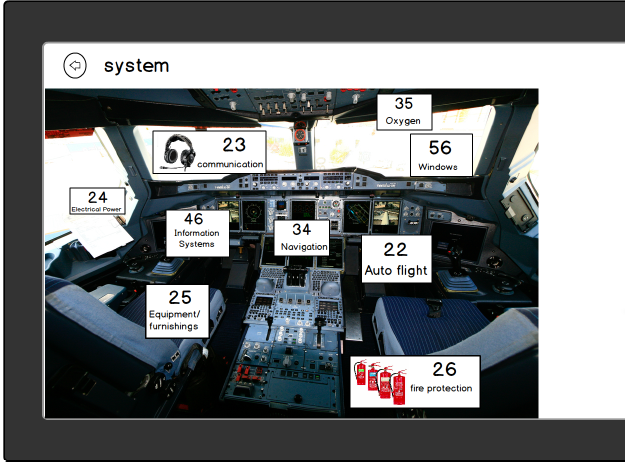
\includegraphics[width=360px]{images/catalogue_entwurf}
\caption{Entwurf der Produktkategorie Auswahl}
\label{catalogueSketch}
\end{figure}
Abbildung \ref{catalogueSketch} zeigt die Zuteilung der Kategorien auf die einzelnen Bereiche im Flugzeug. Wichtig hierbei ist das Verwenden von ansprechenden Bildern und großen Auswahlboxen. Der Kunde muss die benötigten Upgrades den einzelnen Bereichen zuordnen können und kann mit der Anwendung schnell zu seinem benötigten Produkt navigieren. Mit der Darstellung wird das Ziel erreicht, den Kunden für die Komplexität des Produktes zu sensibilisieren und ihm gleichzeitig eine bessere Suchmöglichkeit als über Produkt- oder Kategorienummern zu ermöglichen. \par 

Nach der Auswahl einer Kategorie wird nach dem in Abschnitt \ref{usingConcepts} vorgestellten Prinzip der hierarchischen Navigation eine Detail Seite angezeigt. Diese enthält die Details über die Upgrademöglichkeiten. Die Struktur beim Katalog des Anwendungsbeispiels enthält eine weitere Unterkategorie, welche im Entwurf (siehe Abbildung \ref{detailSketch}) auf der linken Seite als Liste dargestellt ist. Nach der Auswahl eines dieser Elemente werden auf der rechten Seite die möglichen Upgrades der gewählten Unterkategorie angezeigt. Zusätzlich werden Informationen über die vorhandenen Möglichkeiten und optional Bilder für die Erklärung dargestellt.  Für jedes vorhandene Upgrade in einer Unterkategorie werden einzelne Kacheln verwendet. Diese können per Klick selektiert werden. Die Informationen über das jeweilige Upgrade sind in der Kachel enthalten, ebenfalls ein Produktbild und ggf. der Name des Herstellers. Diese Elemente sind immer auf dem ersten Bildschirm ohne Scrollen sichtbar. Der Benutzer sollte nur bei Bedarf von mehr Informationen scrollen müssen. Hierdurch wird eine schnelle Auswahl der gewünschten Upgrades ermöglicht. 
\begin{figure}[H]
\centering
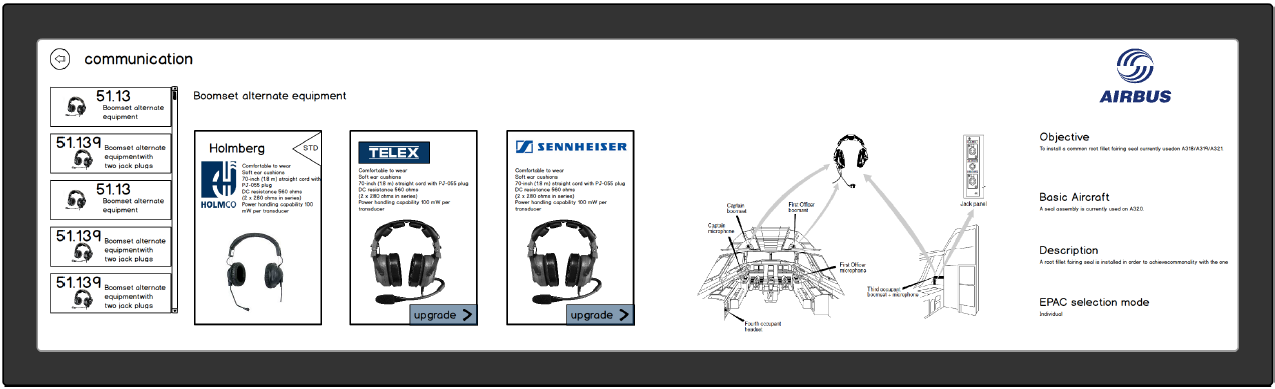
\includegraphics[width=\hsize]{images/detail_entwurf}
\caption{Entwurf der Produktdetail Ansicht}
\label{detailSketch}
\end{figure}

\subsection{Flugzeugauswahl}
Die Auswahl der Flugzeuge ist aufgrund der Voraussetzung für die Konfiguration eine Hauptaufgabe. Für eine schnelle Selektion müssen die Daten zuvor gefiltert werden. Dadurch, dass die Anwendung beim Kunden direkt verwendet wird, sind auch nur dessen Daten relevant. Der Kunde verwendet für die Auswahl die sogenannte Flugzeugversion. Bei der Bestellung von neuen Flugzeugen werden diese in eine neue Version eingeordnet. Jede Flugzeuggesellschaft erhält ein Kürzel, worauf eine Nummer für die Version folgt. Bei der Auswahl der Flugzeuge wird diese Kategorisierung beibehalten. Die vorhandenen Datenelemente werden anhand der Flugzeugversion sortiert. \par

\begin{figure}
\centering
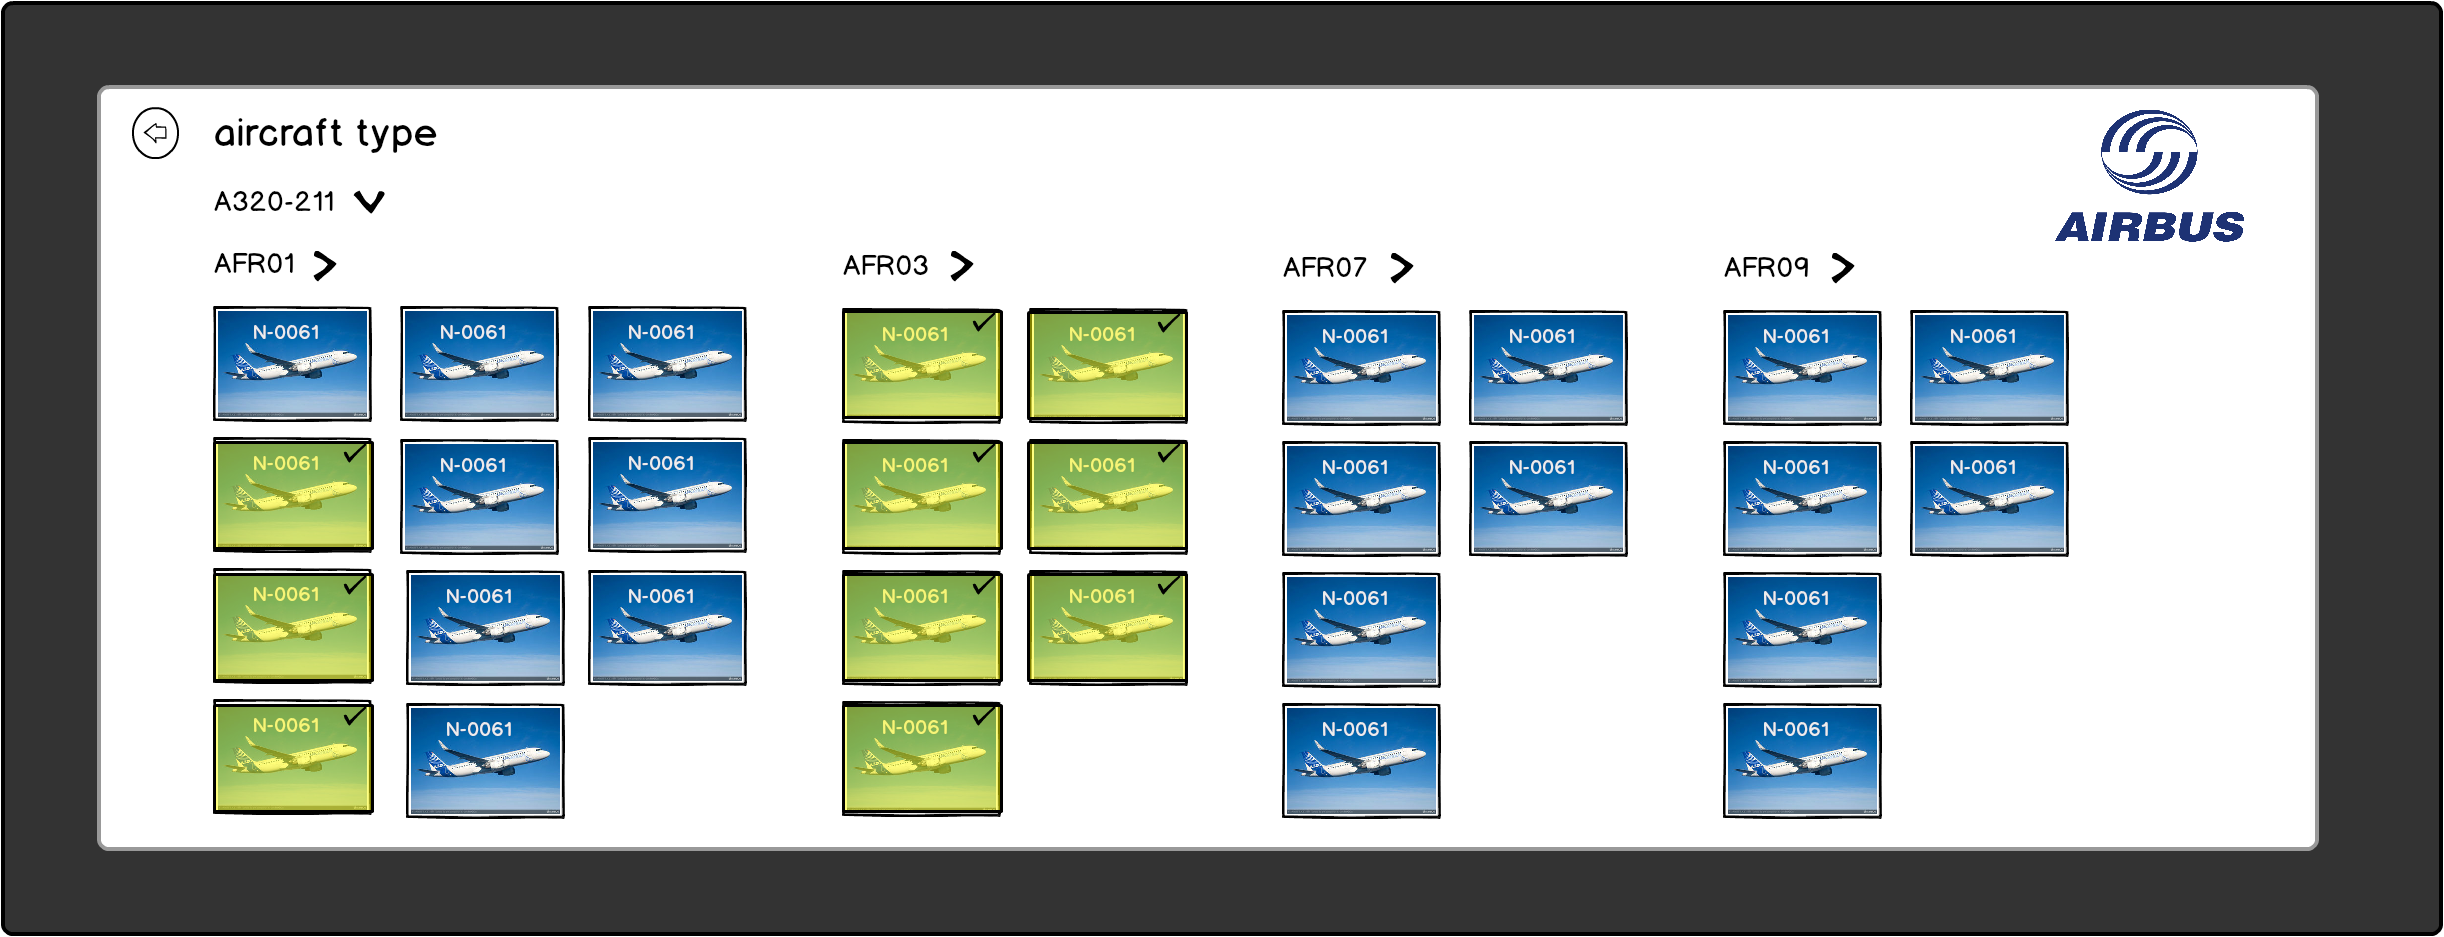
\includegraphics[width=\hsize]{images/version_entwurf}
\caption{Entwurf der Flugzeugauswahl}
\label{aircraftSketch}
\end{figure}
Die Darstellung der einzelnen Flugzeuge erfolgt, wie in Abbildung \ref{aircraftSketch} zu sehen, im Grid. Die einzelnen Flugzeuge werden in einer Kachel angezeigt, wobei jede auswählbar ist. Die Sortierung der Daten erfolgt mit den Versionen als Überschrift der jeweiligen Gruppe. Damit die Daten schneller gefunden werden können, wird ein zusätzlicher Filter verwendet. Dieser soll die Flugzeuge nach dem jeweiligen Typ filtern und so für eine besser Übersicht sorgen. Der Filter wird über den Daten platziert und soll vom Scrollen ausgeschlossen werden. \par 

Damit ein Experte beim Bedienen der Anwendung die Daten schneller auswählen kann(siehe N2), wird der semantische Zoom für diesen Datensatz verwendet. Die herausgezoomte Ansicht enthält die Versionen als Kategorie in einem Grid dargestellt. 

\subsection{Konfigurationsergebnisse}
Die Ergebnisse der Konfiguration werden im modellierten Workflow nach erfolgter Auswahl von Ugrades und Flugzeugen angezeigt. Das Ergebnis besteht aus den gebildeten Konfigurationsgruppen. Beim Entwurf sollen die Gruppen in der Zusammenfassungsseite zu sehen sein, sobald mindestens ein Flugzeug und ein Upgrade ausgewählt wurde. Die Kommunikation mit dem Konfigurationsserver läuft hier automatisch im Hintergrund, so dass jederzeit die Ergebnisse live angezeigt werden. \par
\begin{figure}
\centering
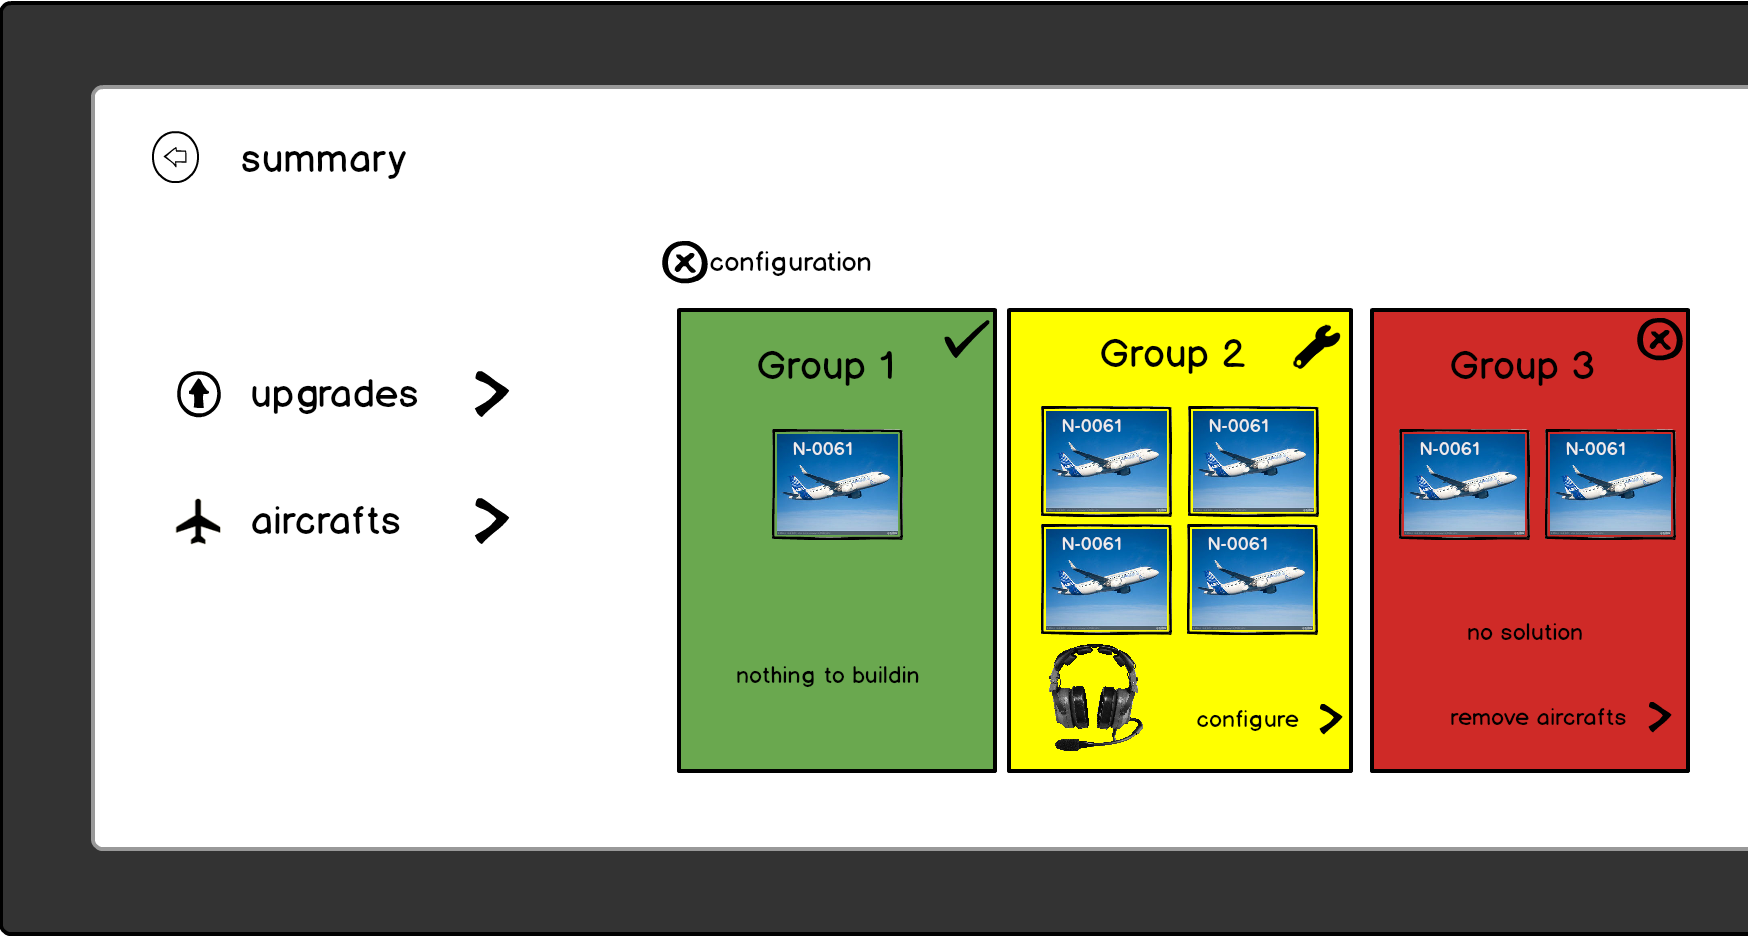
\includegraphics[width=\hsize]{images/configuration_entwurf}
\caption{Darstellung der Konfigurationsergebnisse}
\label{confSketch}
\end{figure}
 Für die Unterscheidung der verschiedenen Konfigurationsstatus werden verschiedene Farben verwendet (siehe Abbildung \ref{confSketch}). Die Darstellung erfolgt nach der Ampel Semantik. Rot bedeutet in diesem Zusammenhang, dass die Konfiguration für bestimmte Flugzeuge nicht durchführbar ist. Bei gelb müssen Alternativen ausgewählt werden, damit der grüne Status einer vollständigen Konfiguration für diese Gruppe erreicht wird. Die einzelnen Kacheln der Konfigurationsgruppen erhalten zusätzliche Icons, anhand derer ebenfalls eine Identifikation des Status abgelesen werden kann. Bei der Auswahl einer Konfigurationsgruppe gelangt man in die Alternativenauswahl. \par
 
 Die Seite für die Auswahl der Alternativen enthält eine kleine Zusammenfassung der Upgrades und Flugzeuge. Für jede Alternative wird eine selektierbare Kachel angezeigt. Nach der Auswahl wird der Status der Konfigurationsgruppe geändert und die Konfiguration kann abgeschlossen werden, wenn alle Gruppen grün sind.

\subsection{Weitere Ansichten}
Der Entwurf für die Hautfunktionen Upgradeauswahl, Flugzeugauswahl und Konfigurationsergebnisdarstellung ist abgeschlossen. Für die Umsetzung der funktionalen Anforderungen müssen weitere Ansichten hinzugefügt werden. Damit ein Speichern und Laden (F5) ermöglicht wird, soll eine Startseite verwendet werden. 

Diese ist bereits im modellierten Workflow vorgesehen. Von der Startseite aus gelangt man in eine neue Konfiguration oder kann eine bereits vorhandene laden. Sie wird beim Start der Anwendung angezeigt. Somit ist diese Ansicht bei jeder Verwendung der App zu sehen. Aus diesem Grund ist das Design der Startseite wichtig. \par
\begin{figure}[H]
\centering
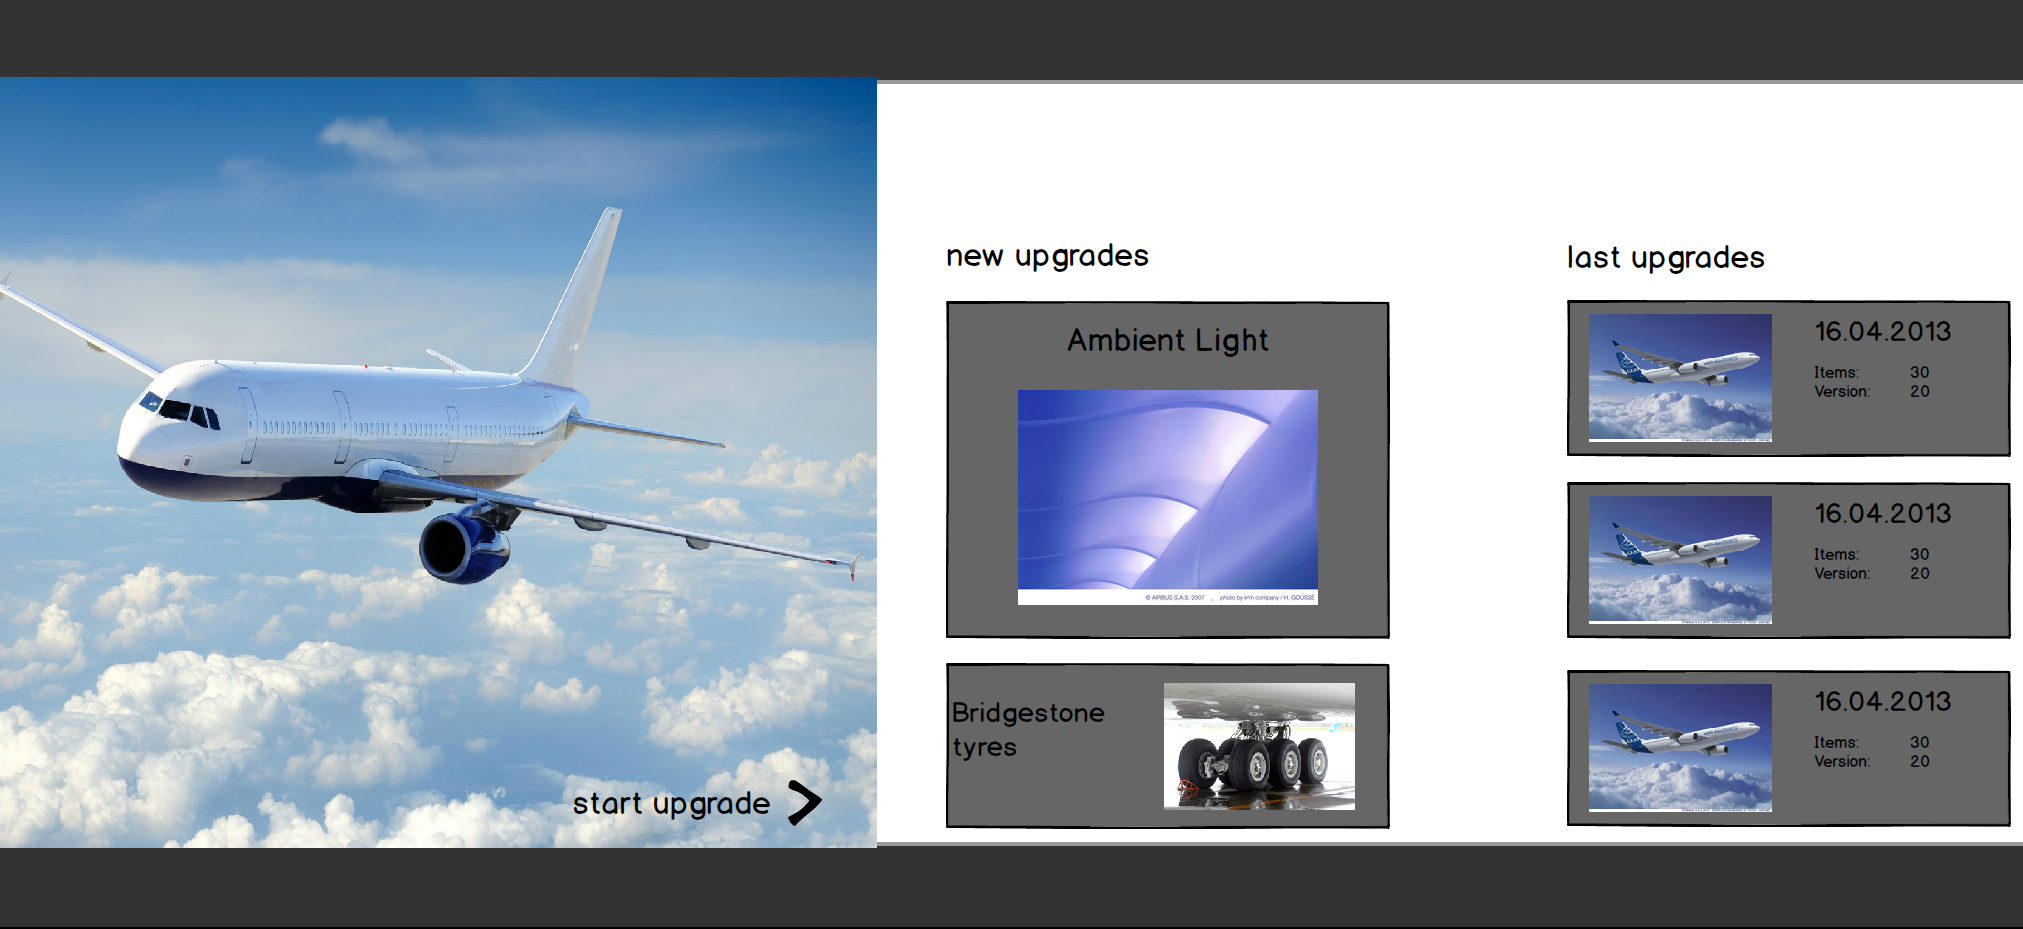
\includegraphics[width=\hsize]{images/start_entwurf}
\caption{Entwurf der Startseite}
\label{startSketch}
\end{figure}
Die Idee ist es, eine kundenspezifische Startseite zu gestalten. Dies sorgt für eine Dynamik in der Seitenanzeige. Der Inhalt ist vom jeweiligen Kunden abhängig. Dies wird zuerst durch ein kundenspezifisches Bild zu Beginn erreicht (siehe Abbildung \ref{startSketch}). Bei der Auswahl des Bildes wird eine neue Konfiguration gestartet. Die Größe wird so gewählt, dass die letzten Konfigurationen erst durch ein scrollen komplett angezeigt werden. Hierdurch wird die Hauptfunktion schneller zugänglich und  die Microsoft Richtlinien der Konzentration auf das Wesentliche werden berücksichtigt. Als zweites Merkmal des Kunden wird das Logo der Fluggesellschaft am oberen linken Rand angezeigt. Für einen schnelleren Einstieg in die Anwendung werden neue oder für die Fluggesellschaft interessante Upgrades zusätzlich auf der Startseite angezeigt. Bei einem Klick auf diese Kachel wird die Detail Seite geöffnet, so dass mehr Informationen angezeigt werden und eine Auswahl möglich ist. 
\par 

Für die Umsetzung der funktionalen Anforderung F6, die das Filtern der Anwendungsdaten spezifiziert, wird eine weitere Ansicht benötigt. Die Daten sind in der Flugzeugauswahl und in der neuen Startseite auf einen Kunden beschränkt. Andere Datensätze werden nicht benötigt.  Das Problem mit der Filterung kann aus diesem Grund mit einer Kundenauswahl gelöst werden. Diese Auswahl stellt im Anschluss alle kundenspezifischen Daten der Anwendung bereit und erfüllt die Anforderung eines entsprechenden Filters. \par 

Die Ansicht für die Auswahl der Kunden wird analog zu der Flugzeugauswahl gestaltet. Es wird hier ebenfalls für jeden Kunden eine eigene Kachel angezeigt. Diese sind im Grid angeordnet. Eine Einteilung in Kategorien erfolgt Alphabetisch. Im Anwendungsbeispiel sind sehr viele Kunden vorhanden. Damit eine schnelle Auswahl erfolgen kann, wird der Semantische Zoom in der Ansicht verwendet. Die Kategorisierung erfolgt über das Alphabet. Es kann jedem Buchstaben ein Kunde zugeordnet werden. Nach der Auswahl eines Datums durch den Experten werden die kundenspezifischen Anwendungsdaten auf das mobile Endgerät geladen und können anschließend beim Kunden "'offline"' verwendet werden. \par 

Die zweite Filterung der Daten wird über die Programmauswahl realisiert. Diese Auswahl wird beim Starten einer neuen Konfiguration von der Startseite aus aufgerufen. Der Programmfilter wählt den richtigen Produktkatalog aus und verringert die Menge der vorhandenen Flugzeuge. Bei der visuellen Darstellung der Ansicht werden die vier möglichen Programme angezeigt. Damit der Kunde die Programmauswahl versteht, wird für jedes Programm ein passendes Flugzeugbild gewählt. Für die Umsetzung der "'Content over Chrome"' Richtlinie erhalten die vier Kacheln eine Bildschirmfüllende Größe, so dass die Auswahl mit Touch vereinfacht wird.


\section{Navigation und Bedienung}
Alle benötigten Ansichten sind den Anforderungen entsprechend konzipiert. Damit die Anforderung einer einfachen Bedienung (N1) erfüllt ist, muss ein passendes Navigationskonzept erstellt werden. Die Navigation unterstützt den Benutzer, indem es Fehler bei der Anwendung verzeiht. Hierzu gehört beispielsweise ein schnelles Zurückspringen nach einer falschen Auswahl. Weiterhin muss ein schneller Ablauf des normalen Anwendungsfalls unterstützt werden. Der modellierte Workflow ist die Ausgangsbasis der Navigation. Dieser wird mit den zusätzlichen Ansichten und neuen Navigationsmöglichkeiten erweitert. \par 

\subsection{Navigationsverlauf}
\begin{figure}[H]
\centering
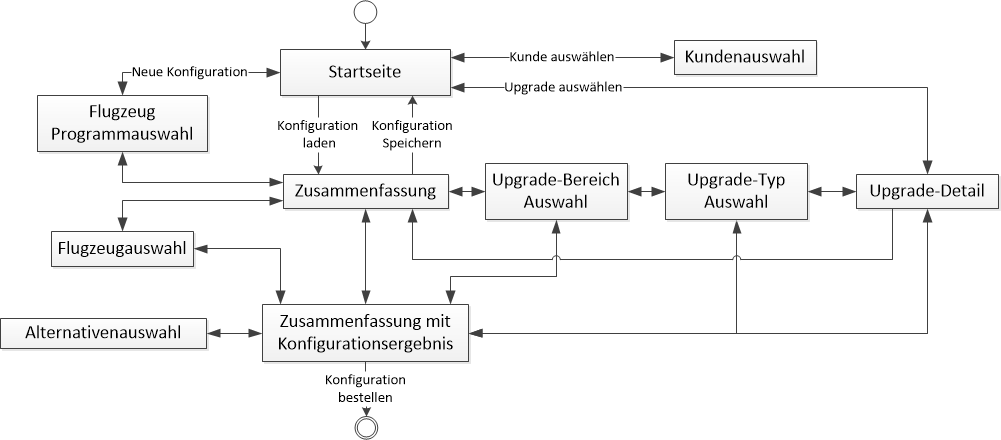
\includegraphics[width=\hsize]{images/workflow_navigation}
\caption{Navigation in der App}
\label{appNavigation}
\end{figure}
Abbildung \ref{appNavigation} zeigt die Möglichkeiten bei der Navigation. Es wird dabei eine hierarchische Struktur verwendet. Der Ursprungspunkt der Anwendung ist die Startseite. Von ihr können die vier Ansichten Programmauswahl, Zusammenfassung, Upgradedetail und Kundenauswahl erreicht werden.  Nach der Auswahl eines Kunden werden die Kundendaten geladen und es erfolgt ein Rücksprung zur Startseite. Nach Auswahl der drei anderen Möglichkeiten ist das Ziel die Zusammenfassung zu erreichen. Dies wird bei einer neuen Konfiguration erst nach der Auswahl eines Programms möglich. Bei der Selektion eines Upgrades wird von der Detailseite aus zurückgesprungen. Aus der Zusammenfassung kann in jede Hauptfunktion navigiert werden. Damit ist immer eine Ausgangsbasis vorhanden, anhand der Benutzer sich orientieren kann. Wenn sowohl Flugzeuge, als auch Upgrades ausgewählt sind, werden die Konfigurationsergebnisse in der Zusammenfassung angezeigt. Nachdem die benötigten Alternativen ausgewählt wurden, kann der Konfigurationsprozess durch die Bestellung abgeschlossen werden.
 
\subsection{Bedienelemente}
Damit die oben genannten Navigationsmöglichkeiten umgesetzt werden können, müssen passende Bedienelemente der Zielplattform ausgewählt werden. Hierzu werden folgende vier Möglichkeiten der Navigation eingesetzt: \par

\textbf{Auswahl durch Kacheln:} Zu den Hauptfunktionen der Anwendung wird mit großen Auswahlflächen navigiert. Diese besitzen ein aussagekräftiges Icon und werden direkt auf der Oberfläche angezeigt (siehe Entwürfe).  

\textbf{Obere AppBar:} Für die Navigation zu allen wichtigen Ansichten wird zusätzlich eine Möglichkeit in der oberen AppBar gegeben. Über dieses Bedienelement kann zu der Startansicht, Flugzeugauswahl, Upgradeauswahl und Zusammenfassung navigiert werden (Abbildung \ref{upperApp}). Diese Navigationsmöglichkeit ist in jeder Ansicht möglich und hilft dem erfahrenen Benutzer bei einer schnellen Bedienung (N2). \par
\begin{figure}[H]
\centering
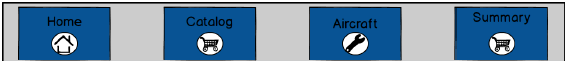
\includegraphics[width=\hsize]{images/UpperAppBar}
\caption{Obere AppBar für die Navigation}
\label{upperApp}
\end{figure}
\textbf{Untere AppBar:} Die Kundenauswahl ist nur für den Vertriebsexperten oder den Hersteller von Interesse. Aus diesem Grund wird die Navigation von der Startseite aus über die untere AppBar (siehe \ref{lowerApp}) ermöglicht.  Weiterhin wird diese Leiste für ein schnelles Navigieren von der Detailansicht zur Zusammenfassung verwendet . Nach der Auswahl eines Upgrades wird durch einen Klick auf den entsprechenden Menüeintrag (rechter Button im Bild) in der unteren AppBar  der Auswahlvorgang abgeschlossen und es erfolgt eine Navigation zur Zusammenfassung.
\begin{figure}[H]
\centering

\includegraphics[width=\hsize]{images/LowerAppBar}
\caption{Untere AppBar für die Navigation}
\label{lowerApp}
\end{figure}
\textbf{Zurück Button:} In jeder Ansicht, außer der Startseite, wird dem Benutzer das Zurückkehren zur vorigen Ansicht ermöglicht. Hierdurch kann eine unbeabsichtigte Navigation schnell rückgängig gemacht werden.

\section{Expertenmodus}\label{expertDesign}
Die Anforderung einer schnellen Bedienung ist mit einem komplexen Navigationskonzept erfüllt. Damit nach der Heuristik einer flexiblen Nutzung weitere Möglichkeiten bei der Anwendung existieren, werden weitere Konzepte für die Erfüllung der Anforderung benötigt. Bisher wurden nur die Bedürfnisse des Endkunden berücksichtigt. Das primäre Ziel beim Entwurf war es, dass komplexe Produkt zu vereinfachen und die Auswahl auf einem angenehmen Weg durchzuführen. Die zweite Zielgruppe der Anwendung sind weiterhin die Experten. Diese wollen die App auf eine effizientere Weise nutzen können. Da Produktkenntnisse vorhanden sind, können andere Ansätze bei der Navigation eingesetzt werden. Das Ziel des Entwurfs ist es dabei, einen sogenannten Expertenmodus bereitzustellen.


\subsection{Einsatz der Flip View}
Im neuen Navigationsworkflow (siehe \ref{appNavigation}) müssen für die Auswahl eines Upgrades mehrere Vorselektionen durchlaufen werden. Dieser Mechanismus ist für den Kunden ideal, da er so den Aufbau des Produktes sowie die einzelnen vorhandenen Möglichkeiten versteht. Für den Experten, der den Aufbau kennt und genau weiß, was er will, ist dies unnötig. Hier muss eine weitere Möglichkeit geschaffen werden, wie die Auswahl schneller erfolgen kann. \par 

Der Lösungsansatz besteht im Verwenden der Flip View. Dieses Oberflächenelement wird vom Framework bereitgestellt und ermöglicht ein schnelles Wechseln der aktuellen Seite durch eine Wisch Geste. Die Idee ist das Verwenden dieser Komponente in der Upgrade-Bereich Auswahl. 
\begin{figure}
\centering
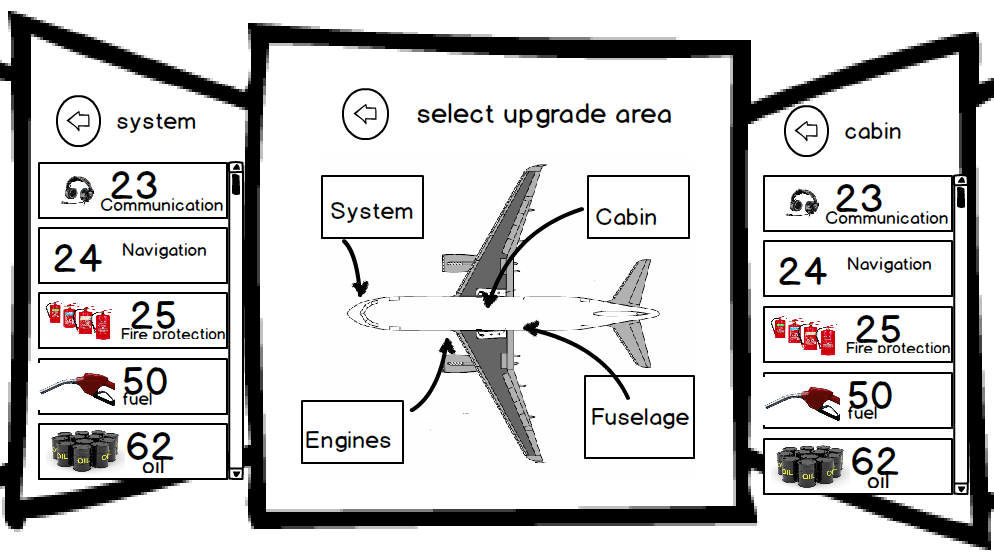
\includegraphics[width=400px]{images/flipView}
\caption{Flip View in der Upgrade Bereich Auswahl}
\label{flip}
\end{figure}
Abbildung \ref{flip} zeigt den Entwurf dieser Ansicht. Der normale Benutzer sieht nur das Bild in der Mitte und kann den gewünschten Flugzeugbereich auswählen, um danach den Upgrade-Typ zu wählen. Für eine schnellere Nutzung kann durch einen Wisch nach rechts oder links eine neue Seite angezeigt werden, die ein Inhaltsverzeichnis mit allen Produktkategorien enthält. Alle Typen lassen sich in die beiden Bereiche System und Cabin einordnen, weshalb nur zwei solcher Verzeichnisse benötigt werden. Der Experte wählt eine Kategorie aus und wird direkt zur Upgradeauswahl navigiert. Damit wird die Typ Auswahl übersprungen und  Upgrades können direkt ausgewählt werden.

\subsection{Erweiterung des Semantischen Zooms}
Die Entwürfe für die Kunden- und Flugzeugauswahl sehen die Verwendung des semantischen Zooms vor. Dieser hilft bei einer schnelleren Auswahl der Flugzeuge. Beim ursprünglichen Entwurf werden die einzelnen Flugzeuge nach den Versionen eines Flugzeuges gruppiert. Damit der Experte auch an dieser Stelle Flugzeuge schneller auswählen kann, wird der semantische Zoom erweitert. Des Weiteren wird eine flexible Nutzung dadurch ermöglicht, dass der Benutzer eine Kategorie selbst festlegen kann. Dies wird mit einer Dropdown Liste im Kopfbereich der Flugzeugauswahl realisiert (siehe \ref{dropdown}). Nach der Auswahl einer Kategorie erfolgt eine Neugruppierung der Datensätze und der semantische Zoom wird somit erweitert. Durch diese Maßnahme erhält der erfahrene Benutzer eine weitere Möglichkeit, die einzelnen Flugzeuge schnell zu finden und somit eine effektive Auswahl durchzuführen.
\begin{figure}[H]
\centering
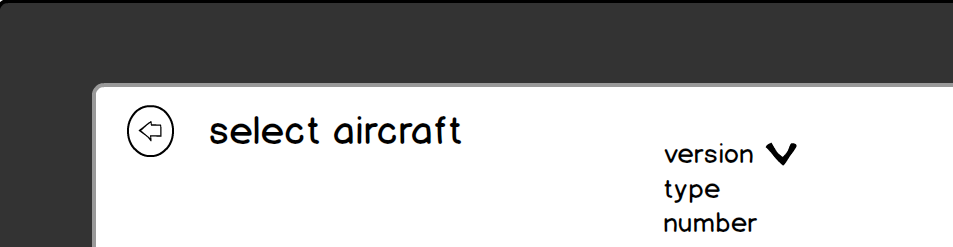
\includegraphics[width=400px]{images/semanticZoom}
\caption{Dropdown List bei der Flugzeugauswahl}
\label{dropdown}
\end{figure}

	\chapter{Implementierung}\label{chapter_5}
 Die Implementierung hat das Ziel die Umsetzung der zuvor entworfenen Ansichten sowie die Realisierung der Anwendung auf der Zielplattform. Im Folgenden wird die Architektur und der Aufbau beschrieben. Anschließend werden die wichtigsten Entscheidungen, die bei der Implementierung getroffen wurden, erklärt.

\section{Anwendungsarchitektur}
Damit die Entwicklung der Anwendung beschleunigt werden kann, indem wiederverwendbare Muster in der Anwendung verwendet werden, wird zuerst eine geeignete Anwendungsarchitektur benötigt. Als erste Voraussetzung muss diese von der Zielumgebung, bzw. von der Technologie unterstützt werden. \par 

Aufgrund des Offline-Modus in der Anwendung sowie die Verwendung des Konfigurationsservers müssen zwei unterschiedliche Formen der Datenanbindung unterstützt werden. Dies hat zur Folge, dass ein einfacher Austausch der Datenanbindung in der Anwendung möglich sein muss, ohne eine Neuimplementierung der Schnittstellen. Die Anforderung an ein ästhetisches Design kann durch eine klare Trennung der Ansicht mit den Logikkomponenten erfüllt werden. Damit ist es möglich, die Gestaltung frei von der notwendigen Logik umzusetzen und sich auf die Gestaltung der Benutzerschnittstelle zu konzentrieren. Die Architektur muss ebenfalls für Erweiterungen offen sein, damit zusätzliche Anforderungen, die beim Einsatz der Anwendung entstehen, umgesetzt werden können.

\subsection{Model-View-ViewModel}
Eine Lösung für die oben genannten Anforderungen an die Architektur bietet das von Microsoft entwickelte Model-View-ViewModel (MVVM) Entwurfsmuster. Hier wird eine strikte Trennung zwischen der Ansicht (View), der Logik (ViewModel) und den Daten (Model) vorgenommen.\par 

\begin{figure}
\centering
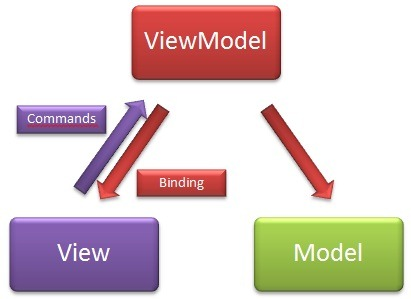
\includegraphics[height=100px]{images/mvvm}
\caption{Komponenten und Kontrollfluss im MVVM Entwurfsmuster}
\label{mvvm}
\end{figure}
Die Kommunikation der einzelnen Komponenten ist in Abbildung \ref{mvvm} dargestellt. Die unterste Ebene ist die Model-Schicht. Diese ist für das Bereitstellen und Persistieren der Daten zuständig. Es wird hierzu entweder eine Datenbank oder Webserviceschnittstelle verwendet. Wichtig bei dieser Schicht, wie in der Abbildung zu sehen, ist der unidirektionale Kontrollfluss mit dem ViewModel. Damit ist eine Manipulation der Daten nur von einer Stelle aus möglich. Dies vereinfacht das Finden von Fehlern. \par
Auf der anderen Seite ist die View. Diese Komponente ist für das Darstellen der Daten zuständig. Es werden alle Oberflächenelemente einer Benutzerschnittstelle auf dieser Ebene verwendet. Die Interaktionen des Benutzers werden auf dieser Anwendungsschicht durchgeführt. Die Auswertung der Eingaben folgt im "'Modell der Ansicht"' \cite[S.9]{bib:mvvm}, dem ViewModel. Diese Schicht ist der Vermittler zwischen den Daten und der Benutzerschnittstelle. Aus diesem Grund werden die Daten, die vom Model erhalten werden für die Ansicht aufbereitet. Die Verbindung zur View-Ebene ist dabei bidirektional, damit sowohl Benutzereingaben, als auch Veränderungen im ViewModel registriert werden. \par

Die Anforderung für einen einfachen Austausch der Datenquelle wird durch die Unabhängigkeit des Models erfüllt. Hierdurch können die Daten sowohl auf dem Gerät, als auch mit Webserviceschnittstellen geladen werden. Das MVVM Entwurfsmuster wird von der Technologie unterstützt und es sind bereits Codebeispiele vorhanden \cite{bib:winMvvm}. Mit der Trennung von View und ViewModel ist ein einfaches Erstellen von Benutzerschnittstellen möglich. Aufgrund der Unabhängigkeit beider Komponenten können diese auch separat entwickelt werden. Hierdurch wird es beispielsweise möglich, dass ein Designer und ein Programmierer unabhängig voneinander arbeiten können. Diese Vorteile sind der Grund für die Entscheidung zur Verwendung des MVVM Design Patterns anstatt des gängigen Model-View-Controlers (MVC), bei dem die View vom Controller abhängig ist und ein unabhängiges Testen der beiden Schichten nicht möglich ist.

\subsection{Anwenden des Entwurfsmusters}
Bei der Implementierung der Anwendung mussten für die Anzeige der Daten immer wiederkehrende Eigenschaften der Datensätze verwendet werden. Ein Beispiel für eine solche Eigenschaft ist der Name oder die Beschreibung eines Flugzeuges oder Upgrades. Da beim MVVM Entwurfsmuster die View nicht auf das Model zugreift, kennt es diese Datenobjekte nicht. Aus diesem Grund muss das ViewModel diese Daten konvertieren und ein neues Objekt bereitstellen. 

Ebenfalls muss bei einer Manipulation oder Auswahl der Daten die Konvertierung rückgängig gemacht werden, damit das Model die Änderungen vornehmen kann. Diese Vorgehensweise hat bei einer Veränderung der Daten zur Laufzeit Vorteile, da das ViewModel den Zeitpunkt der Persistierung entscheiden kann. Im Anwendungsbeispiel ist dies jedoch ein zusätzlicher Aufwand, der nicht benötigt wird, da keine Daten manipuliert werden, sondern eine Auswahl getätigt wird. Die eigentliche Datenbasis wird in der Anwendung nicht verändert.
Für die Vermeidung des zusätzlichen Aufwandes wurde eine neue Komponente eingeführt. Auf diese haben alle drei Ebenen im MVVM Zugriff. In dieser Komponente sind die festen Datenelemente definiert. Es wird nur ein lesender Datenzugriff ermöglicht. Die konkrete Implementierung der Datensätze wird weiterhin im Model vorgenommen. Damit muss keine Konvertierung der Daten erfolgen, um der View einen Zugriff auf die Daten zu geben. \par 
\begin{figure}
\centering
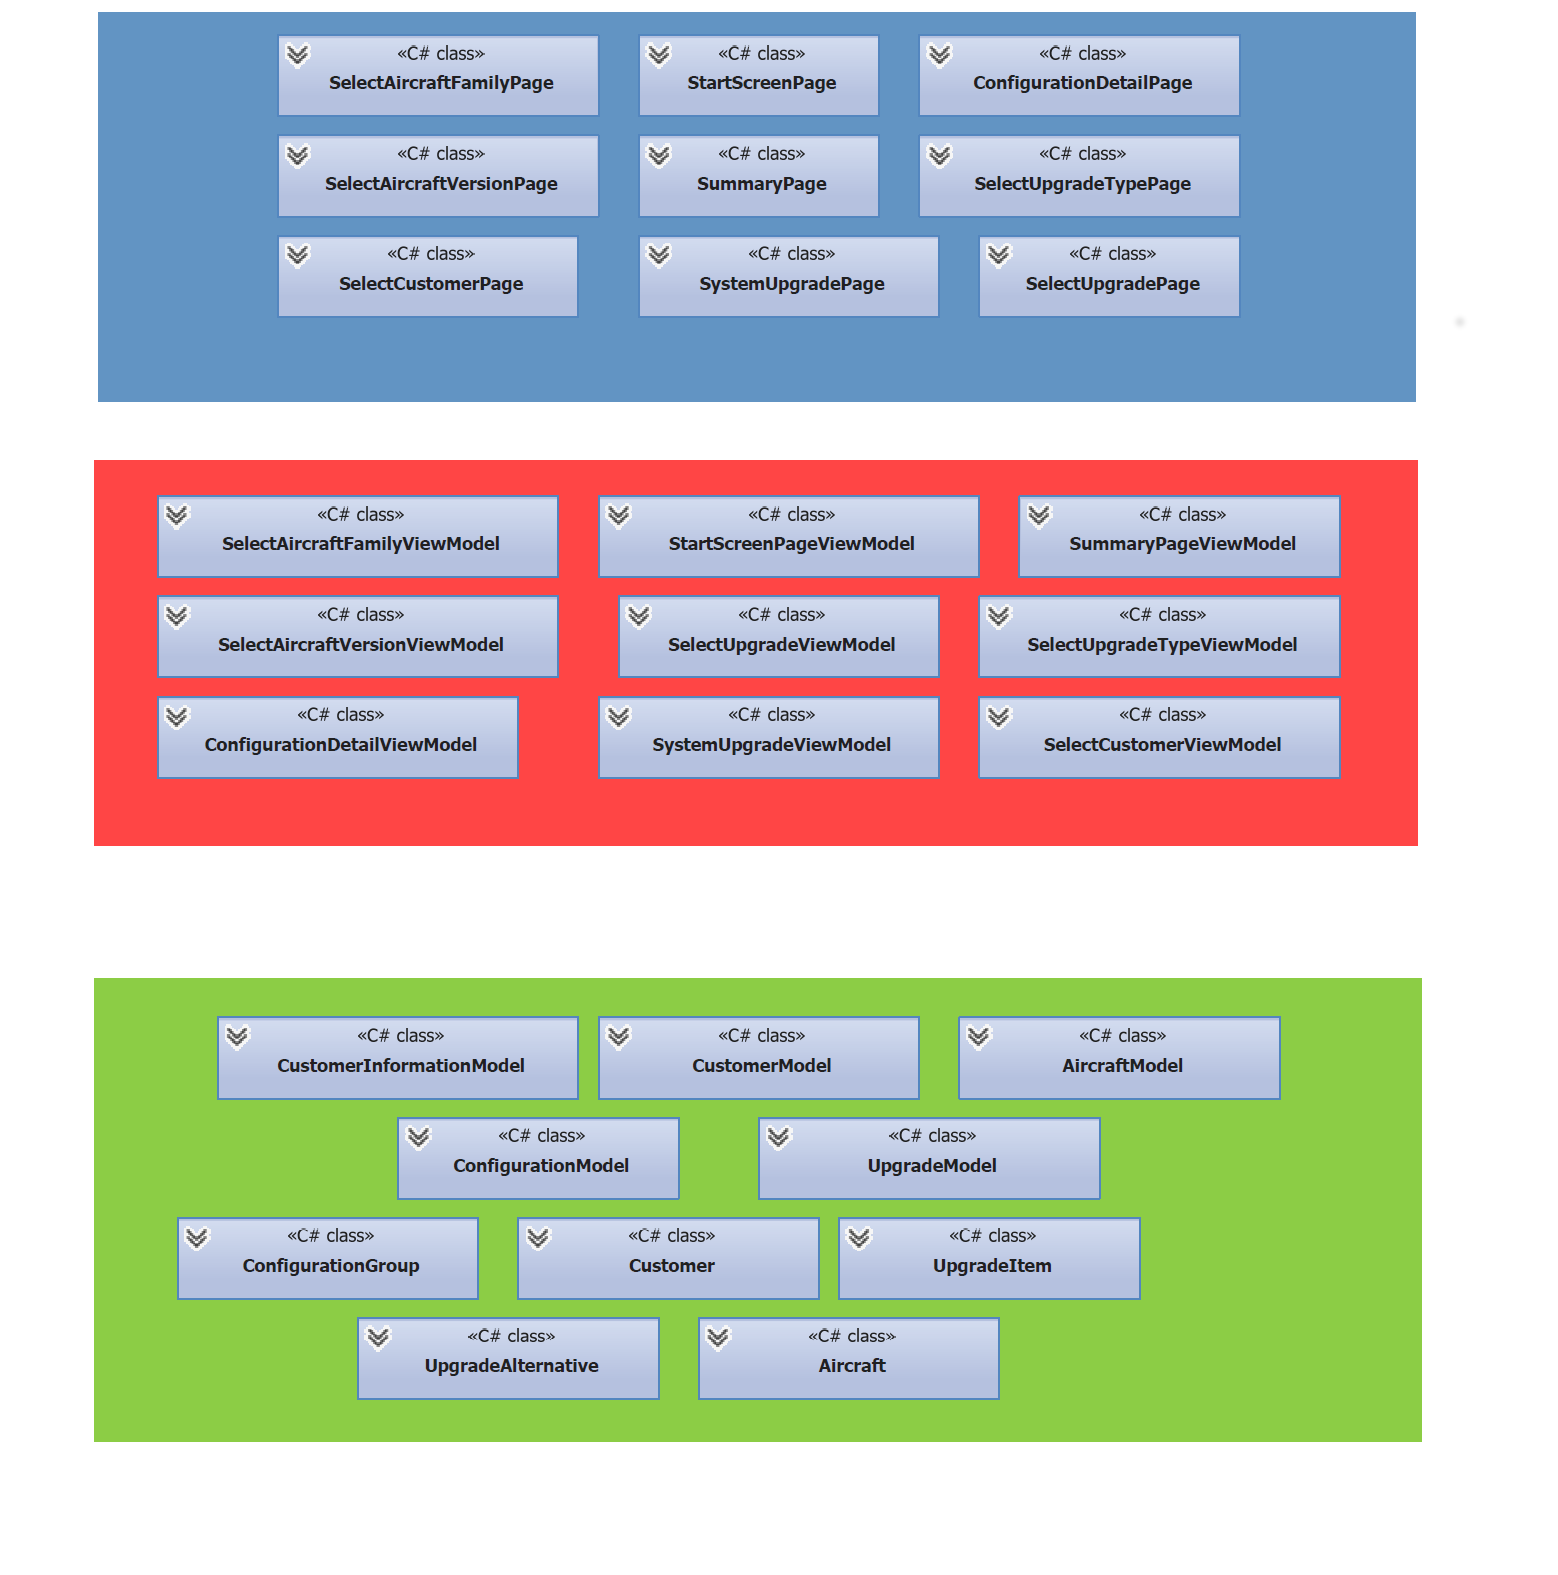
\includegraphics[width=\hsize]{images/uml_diagramm}
\caption{Klassendiagramm im MVVM Entwurfsmuster}
\label{mvvmApp}
\end{figure}
Die Abbildung \ref{mvvmApp} zeigt einen Ausschnitt des Klassendiagramms. Anhand der Auswahl des Upgrades, wie im Navigationsverlauf (siehe \ref{appNavigation}) zu sehen, wird die Anwendung des MVVM Entwurfsmusters demonstriert. Es werden hierfür die drei Ansichten SelectUpgradeTypePage, SystemUpgradePage und SelectUpgradePage benötigt. Alle drei erben von der Klasse Page. Diese ist die vom Framework bereitgestellte Oberflächenklasse und steht für eine Seite der Anwendung. Die Definition der Page und der enthaltenen Oberflächenelemente erfolgt in sogenanntem XAML Code. Dieser ist eine XML-basierte Sprache für das deklarative Erstellen von Benutzerschnittstellen. Alle diese Komponenten lassen sich in die View-Schicht einordnen. \par 

Zu jeder Ansicht existiert ein passendes ViewModel. Damit eine bidirektionale Verbindung aufgebaut werden kann wird für die Kommunikation von der View zum ViewModel sogenannte Bindings verwendet. Ein solches Binding bindet ein Oberflächenelement an das passende Datenelement im ViewModel. Im Beispiel ist das Grid Oberflächenelement an ein Array im ViewModel gebunden. Die Kommunikation in die entgegengesetzte Richtung erfolgt mit Events. Bei einer Änderung der Daten im ViewModel wird ein sogenanntes PropertyChangedEvent ausgeführt. Nachdem die View das Event erhalten hat, werden die Daten in der Ansicht aktualisiert. \par

Für die drei ViewModel Klassen existiert eine gemeinsame Model Klasse. Da die Daten voneinander abhängig sind, ist eine gemeinsame Verwendung sinnvoll. Das Model stellt für jedes ViewModel die passenden Schnittstellen bereit. Die Datenobjekte UpgradeType, SystemUpgrade und Upgrade sind in der Model Schicht vorhanden und werden als Datenbasis verwendet. Die bereitgestellten Methoden verwenden Objekte dieser Klassen. Damit die Datenobjekte auch in der View verwendet werden können, ist die Definition als Interface in die DataCommon Komponente ausgelagert. Diese kann von allen drei Schichten der Anwendung verwendet werden. Im Beispiel wird die Verwendung in den ViewModel Klassen demonstriert. Hier werden die Datenelemente, die für das Binding mit der View benötigt werden als ein Array des Interface bereitgestellt. Dies sorgt für eine einheitliche Kommunikation der drei Ebenen und vermeidet eine Konvertierung der Daten im ViewModel


\section{Navigation}
Eine besondere Herausforderung bei der Implementierung ist die Navigation. Diese muss zuerst in das Entwurfsmuster eingeordnet werden. Es muss entschieden werden, in welcher Ebene navigiert wird. Der Wechsel der Ansichten ist eine Aufgabe der View. Diese bestimmt, wie zu einer neuen Seite navigiert wird. In dieser Ebene werden auch die konkreten Navigationsmethoden angeboten. Andererseits ist die Entscheidung darüber, wann in welche Ansicht gewechselt wird eine Angelegenheit des ViewModels. Diese wertet die Auswahl eines Klicks aus und ist damit für dessen Bearbeitung zuständig. Weiterhin werden Objekte zwischen den beiden ViewModels ausgetauscht. Aus diesem Grund muss es eine Möglichkeit für den Austausch geben. \par 

Die Lösung des Problems erfolgt mit dem Ansatz der Inversion of Control \cite{bib:ioc}. Bei diesem Prinzip geht es um die Auflösung von Abhängigkeiten. Anstatt ein Objekt direkt zu erzeugen, wird es von einer zentralen Stelle verwendet. Die Abhängigkeit wird damit von außerhalb des aktuellen Codes hinzugefügt. Dieser Ansatz hat besonders bei Softwaretests große Vorteile, da andere Objekte für Testzwecke verwendet werden können.  \par
\begin{figure}[H]
\centering
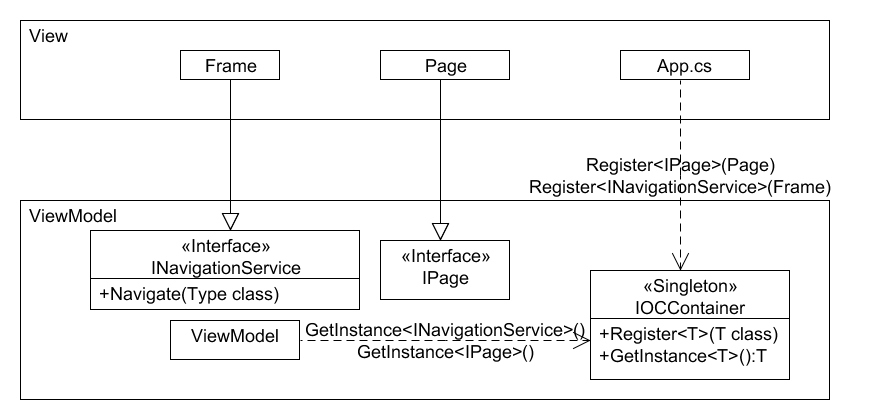
\includegraphics[width=\hsize]{images/dependencyInjection}
\caption{Navigation mit Inversion of Control}
\label{ioc}
\end{figure}
Die Umsetzung des Prinzips ist in Abbildung \ref{ioc} dargestellt. Damit eine Verwendung der einzelnen Klassen aus der View im ViewModel möglich ist, wird für jede Ansicht (Page) ein passendes Interface (IPage) definiert. Eine Navigation wird beim Windows 8 Framework mit der Frame Klasse durchgeführt. Dieses implementiert das INavigationService Interface, welches zwei Navigationsmethoden beinhaltet. Beim Start der App Klasse erfolgt werden die einzelnen Pages und der Navigationsframe mit den definierten Interfaces im IOCContainer registriert. Der Container befindet auf der ViewModel Ebene. Für eine Navigation wird die Zielpage und der Navigationsservice mit der GetInstance<T> Methode erhalten. Anschließend kann die passende Navigationsmethode entweder mit oder ohne Parameter ausgeführt werden. \par 
\begin{figure}[H]
\begin{lstlisting}
private void SaveSelectionAndNavigateToSummaryPage(DataCommon data)
{
       var selectedProgramm = GetSelectedProgramm(data.UniqueId);
       _model.SelectAircraftProgramm(selectedProgramm);
       var classToNavigate = SimpleIoc.Default.GetInstance<ISummary>();
       var navigationService = SimpleIoc.Default.GetInstance<INavigationService>();
       navigationService.Navigate(classToNavigate.GetType());
}
\end{lstlisting}
\caption{Auszug des AircraftFamilyViewModels (siehe Anhang A)}
\label{navigateMethod}
\end{figure}

In Codebeispiel \ref{navigateMethod} wird ein solcher Navigationsvorgang im ViewModel demonstriert. Dieser Auszug ist aus der Flugzeugpgrogramm Auswahl entnommen. Nachdem ein Programm ausgewählt wurde, wird zuerst die Auswahl im Model gespeichert. Im zweiten Schritt erhält man die  Zusammenfassungsseite mit dem Interface (ISummary) vom Container. Die Navigation erfolgt anschließend mit dem Navigationsservice.
\par
Mit diesem Ansatz gelingt es, die Darstellung und die Entscheidung, welche Ansicht bei welchem Inhalt verwendet wird, der View Schicht zu überlassen. Der Wechsel von Ansichten wird mit Methoden durchgeführt, die eine Ansicht bereitstellt. Das ViewModel kann entscheiden, wann eine Navigation durchgeführt wird. Durch die Verwendung des Containers ist eine zentrale Stelle vorhanden, die jederzeit verwendet werden kann. Bei einer Navigation können Parameter übergeben werden, die eine Kommunikation der ViewModels ermöglicht. 

\section{Ergebnisse der Implementierung}
Die Entwürfe des vorigen Kapitels konnten detailreich bei der Implementierung abgebildet werden. Im Folgenden werden die wichtigsten implementierten Ansichten kurz vorgestellt.

\subsection{Startseite und Flugzeugprogrammauswahl}
Das Ergebnis für die Startseite (siehe \ref{startScreenImpl}) konnte vom Entwurf übernommen werden. Für die Anzeige des aktuellen Status der Konfiguration wurde eine Signalfarbe und ein passendes Icon hinzugefügt. Ebenfalls wurde der Text durch passende Icons ausgetauscht (vgl. \ref{startSketch}) 
\begin{figure}[H]
\centering
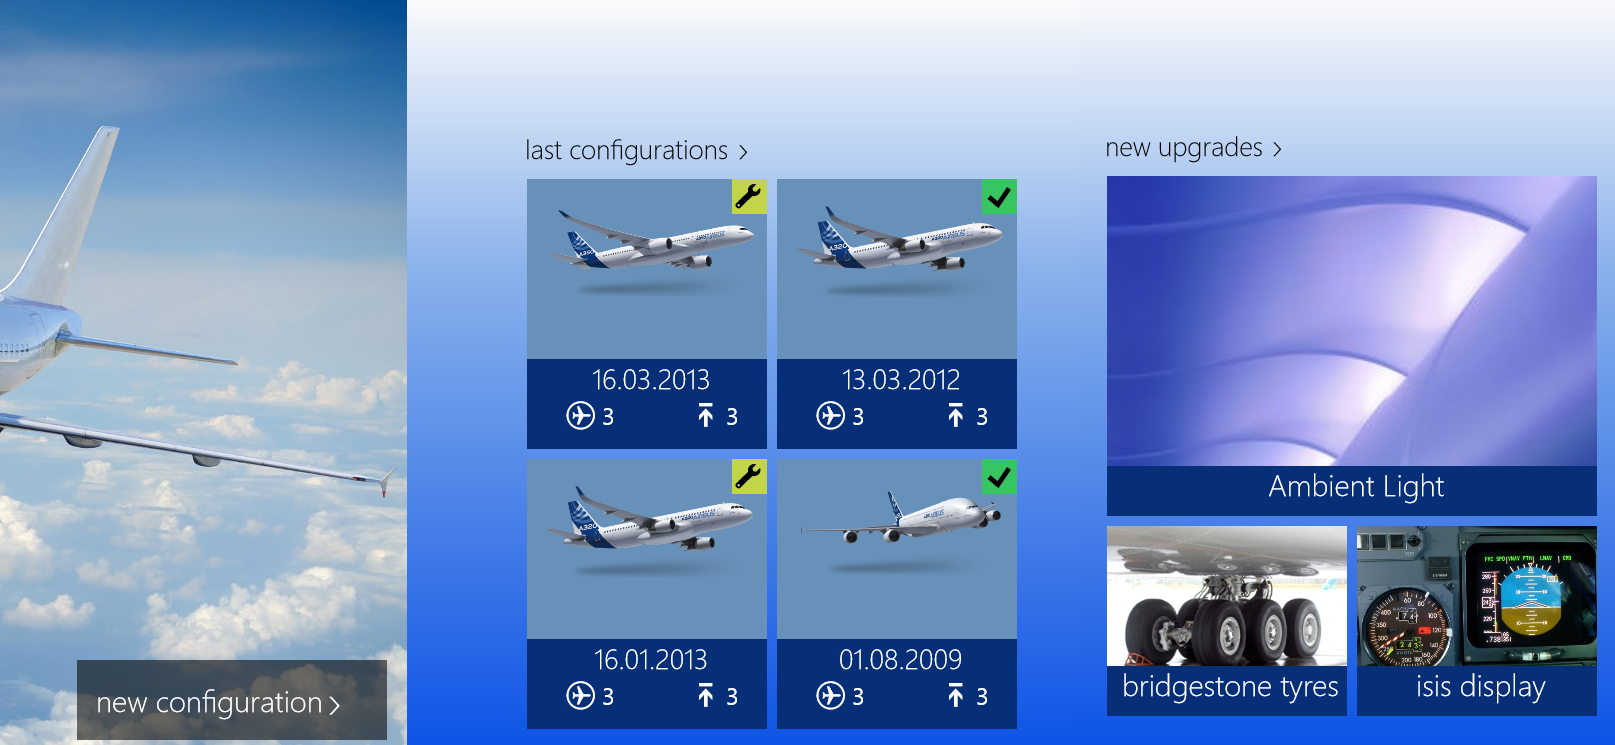
\includegraphics[width=\hsize]{images/impl/start_screen_impl}
\caption{Auszug der implementierten Startseite}
\label{startScreenImpl}
\end{figure}
Bei der Auswahl des Flugzeugprogramms (siehe \ref{aircraftProgrammImpl}), dass direkt nach dem Start einer neuen Konfiguration angezeigt wird, wurde der Begriff Familie statt Programm verwendet. Die Darstellung enthält ein zugehöriges Flugzeug  in der passenden Kachel.
\begin{figure}[H]
\centering
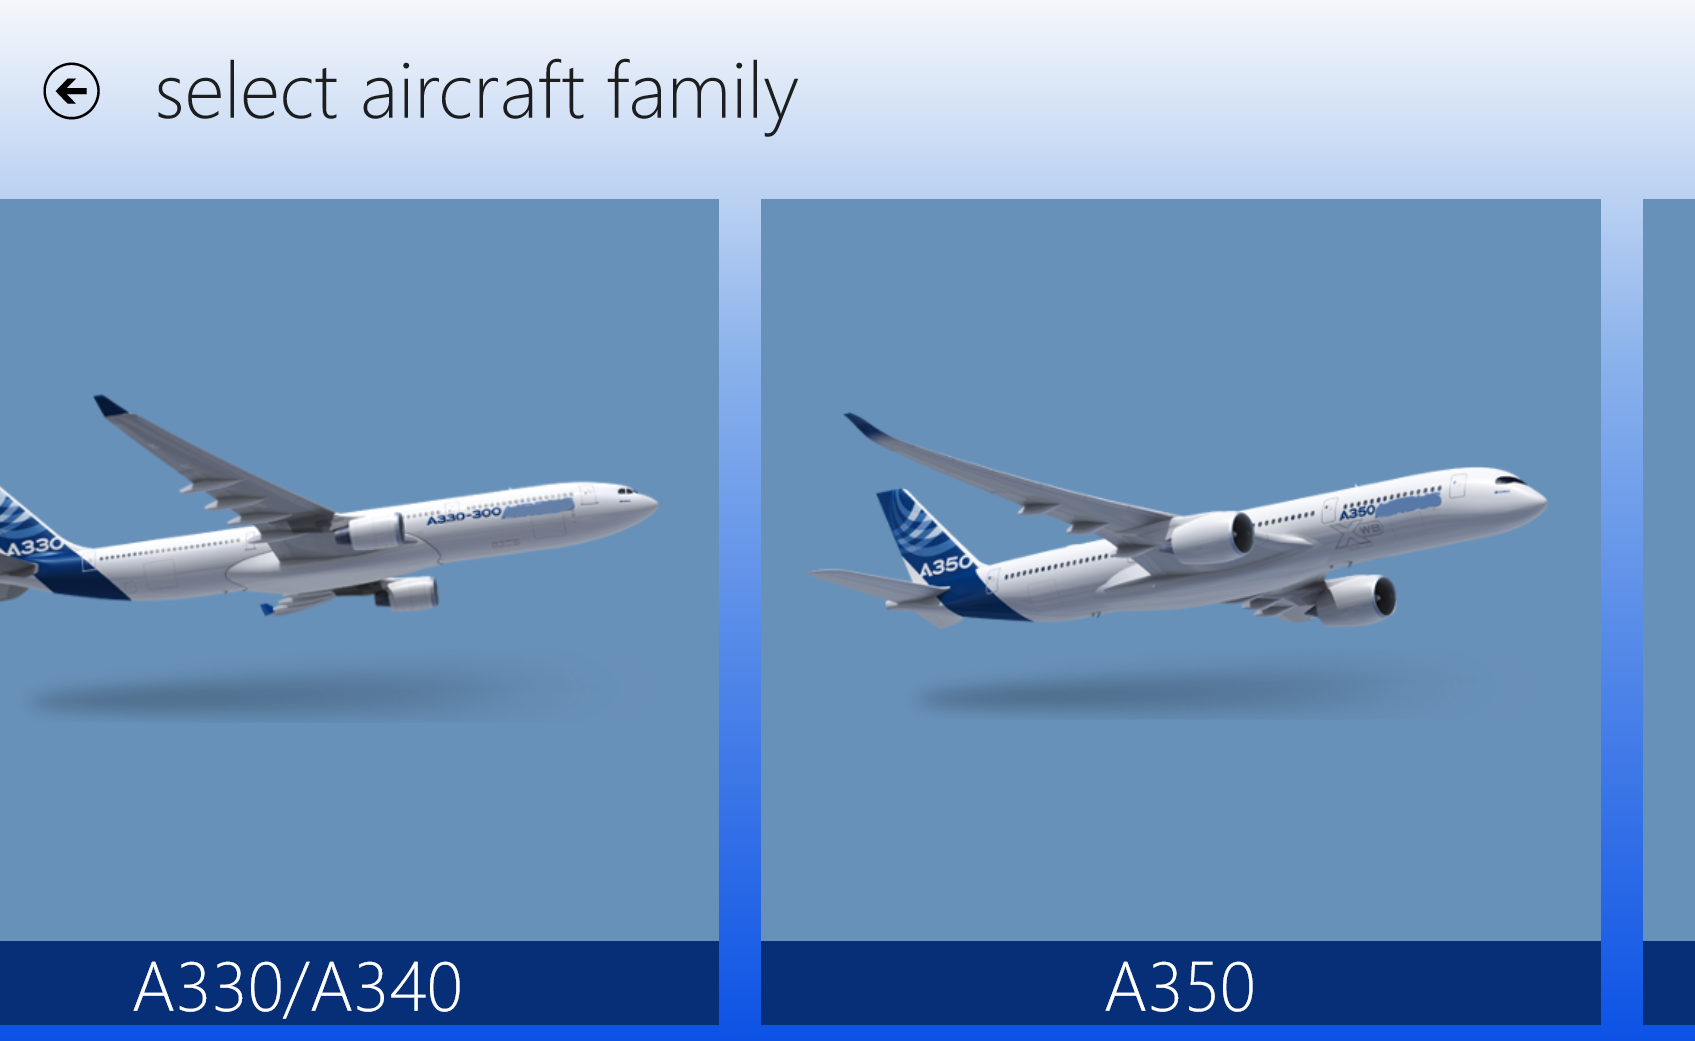
\includegraphics[height=250px]{images/impl/select_aircraft_family_impl}
\caption{Auszug der implementierten Flugzeugprogrammauswahl}
\label{aircraftProgrammImpl}
\end{figure}

\subsection{Upgradeauswahl}
\begin{figure}[H]
\centering
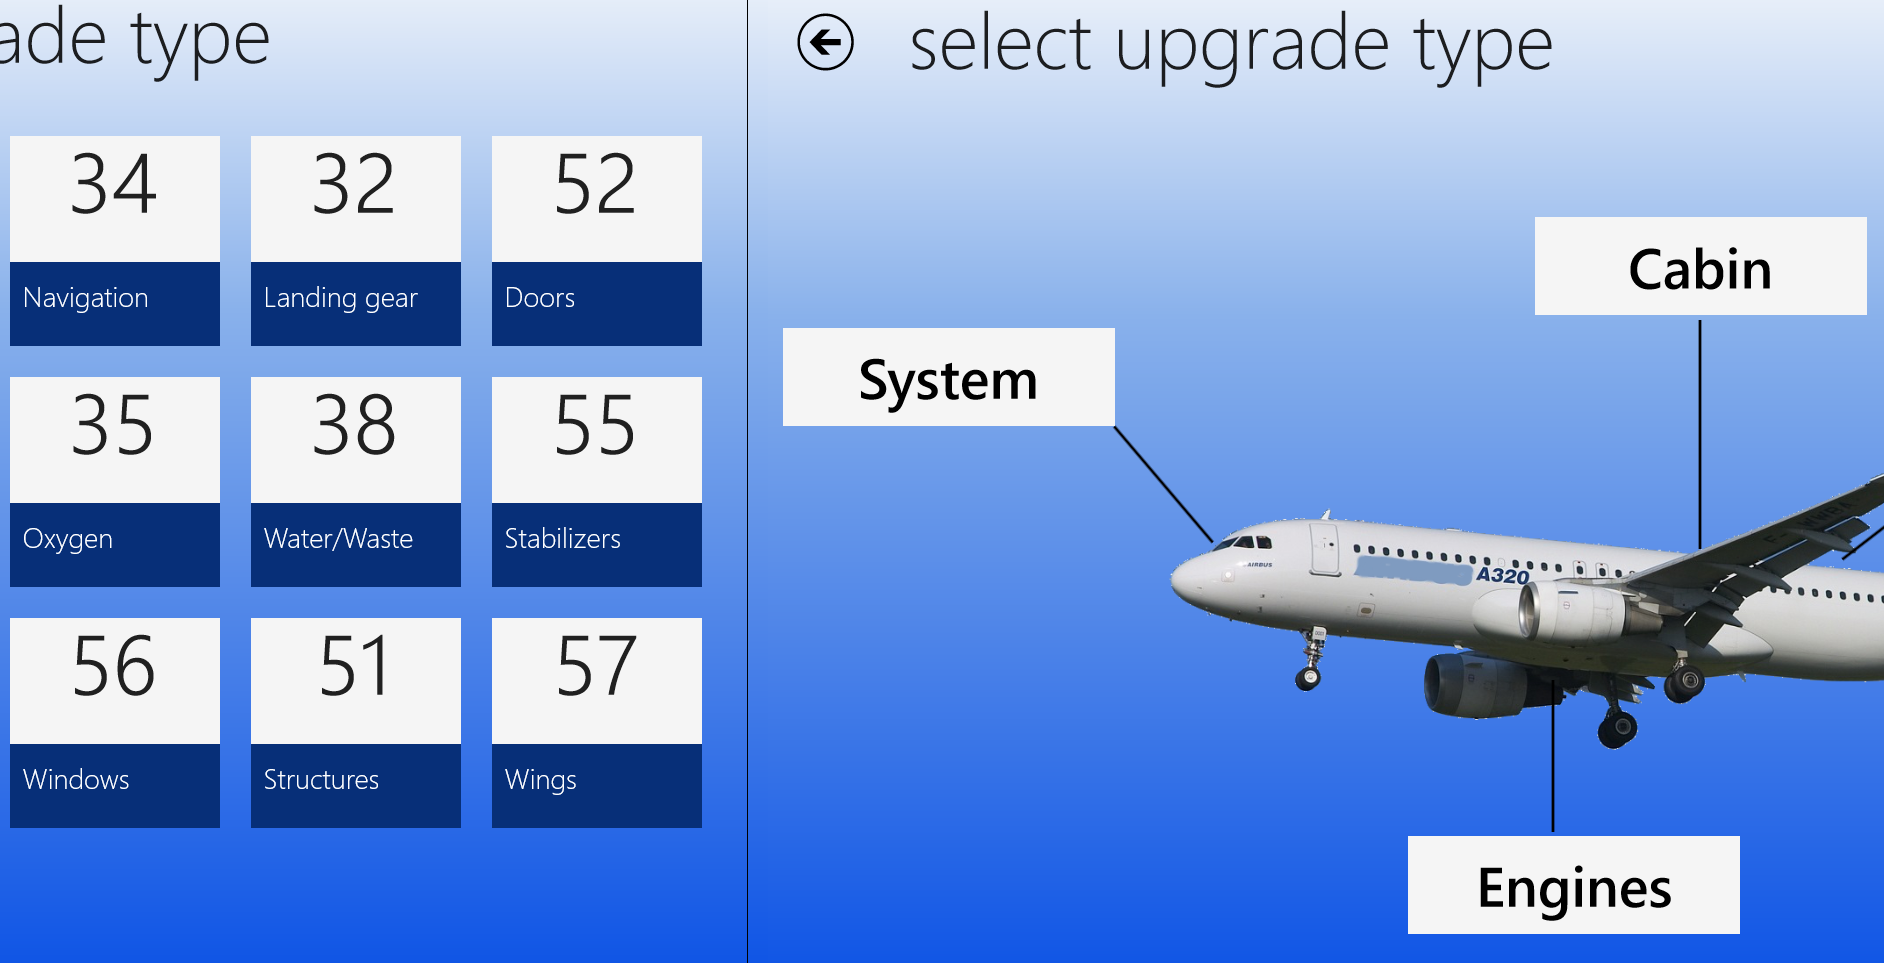
\includegraphics[width=\hsize]{images/impl/select_upgrade_type_impl}
\caption{Auszug der implementierten Upgradetypauswahl}
\label{upgradeTypeSelectionImpl}
\end{figure}
In Abbildung \ref{upgradeTypeSelectionImpl} ist die Auswahl des Upgrade Typs zu sehen. Diese wurde mit der FlipView (vgl. \ref{flip}) umgesetzt. Beim Aufruf der Seite ist die Upgradetyp Auswahl (rechtes Bild) zu sehen.  Um in den Expertenmodus (linke Seite) zu kommen, wird eine Wisch-Geste nach von links nach rechts durchgeführt. Dieses "'flippen"' unterstützt den Experten bei einer schnelleren Navigation.


Bei der Auswahl der Upgrades, wie in Abbildung \ref{upgradeSelectionImpl} zu sehen, sind viele Informationen auf der Ansicht enthalten. Auf der rechten Seite können die einzelnen Unterkategorien ausgewählt werden. Die Details zu der Auswahl erscheinen auf dem rechten Bildschirmrand. Die einzelnen Upgrades werden auf das Wesentliche reduziert. Nach der erfolgten Auswahl wird die derzeitige Selektion auf der unteren AppBar angezeigt. Ein Abschluss der Auswahl sowie die Navigation in die Zusammenfassungsseite erfolgt mit einem Button. \par 
\begin{figure}[H]
\centering
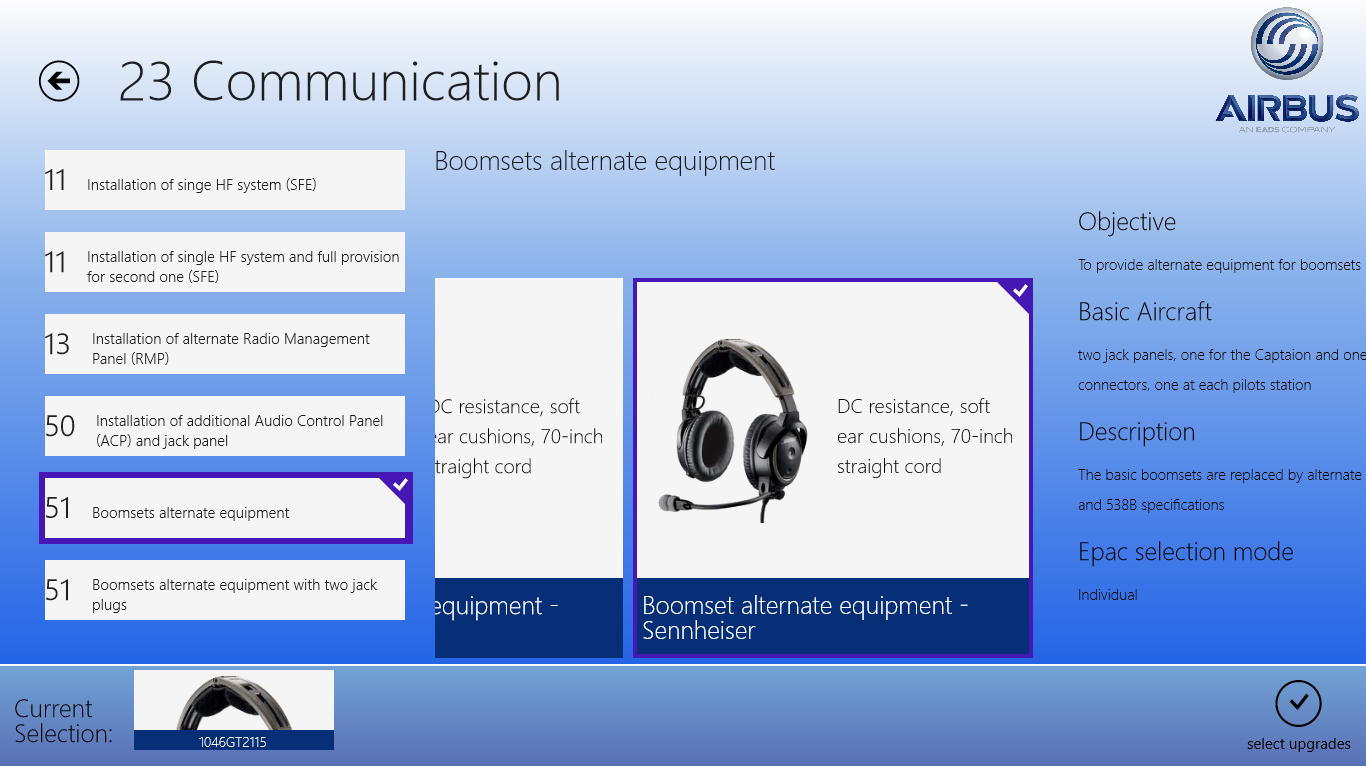
\includegraphics[width=\hsize]{images/impl/select_upgrade_impl}
\caption{Auszug der implementierten Upgradeauswahl}
\label{upgradeSelectionImpl}
\end{figure}

\subsection{Flugzeugauswahl}
Die Auswahl der Flugzeuge (siehe \ref{aircraftSelectionImpl}) ist mit den Kacheln im Grid umgesetzt worden. Für eine schnelle Auswahl von großen Datensätzen wurde der semantische Zoom in dieser Ansicht verwendet. Damit dem Benutzer mehr Möglichkeiten gegeben werden, kann er die Gruppierung der Flugzeuge mit eine Auswahlliste selbst festlegen. Abbildung \ref{aircraftSelectionZoomImpl} zeigt den semantischen Zoom mit den verschiedenen Flugzeugtypen gruppiert.  In dieser Ansicht wird die Anzahl der Elemente in der Gruppe angezeigt. 
\begin{figure}[H]
\centering
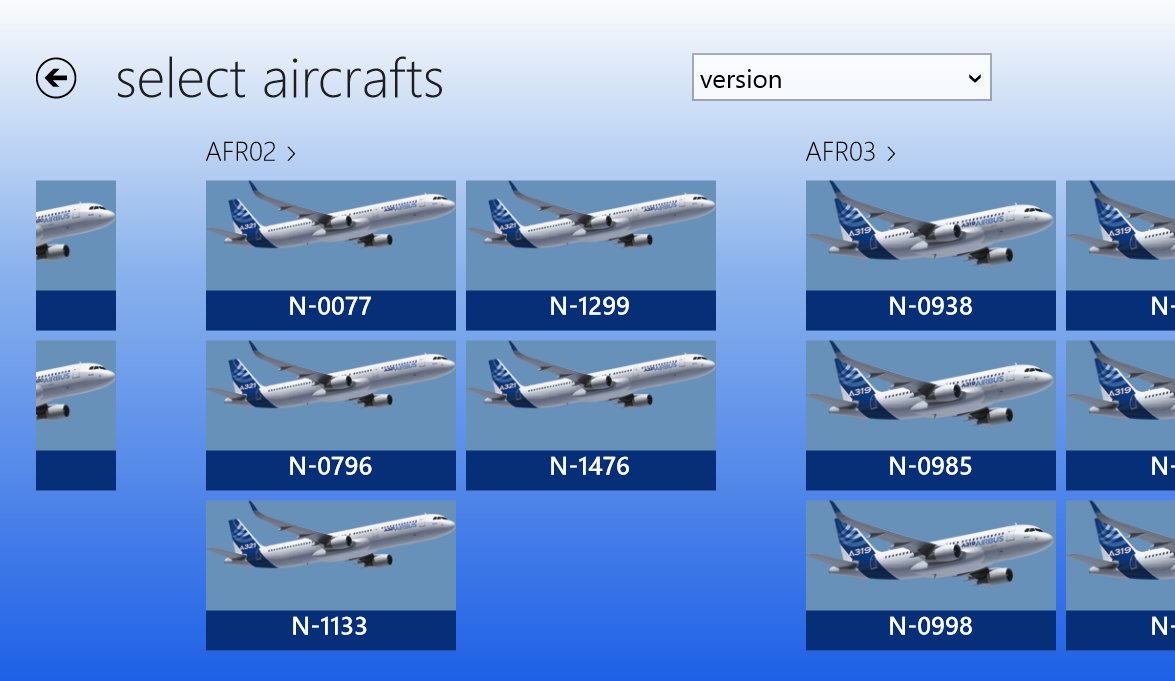
\includegraphics[width=\hsize]{images/impl/select_aircrafts_impl}
\caption{Auszug der implementierten Flugzeugauswahl}
\label{aircraftSelectionImpl}
\end{figure}
\begin{figure}[H]
\centering
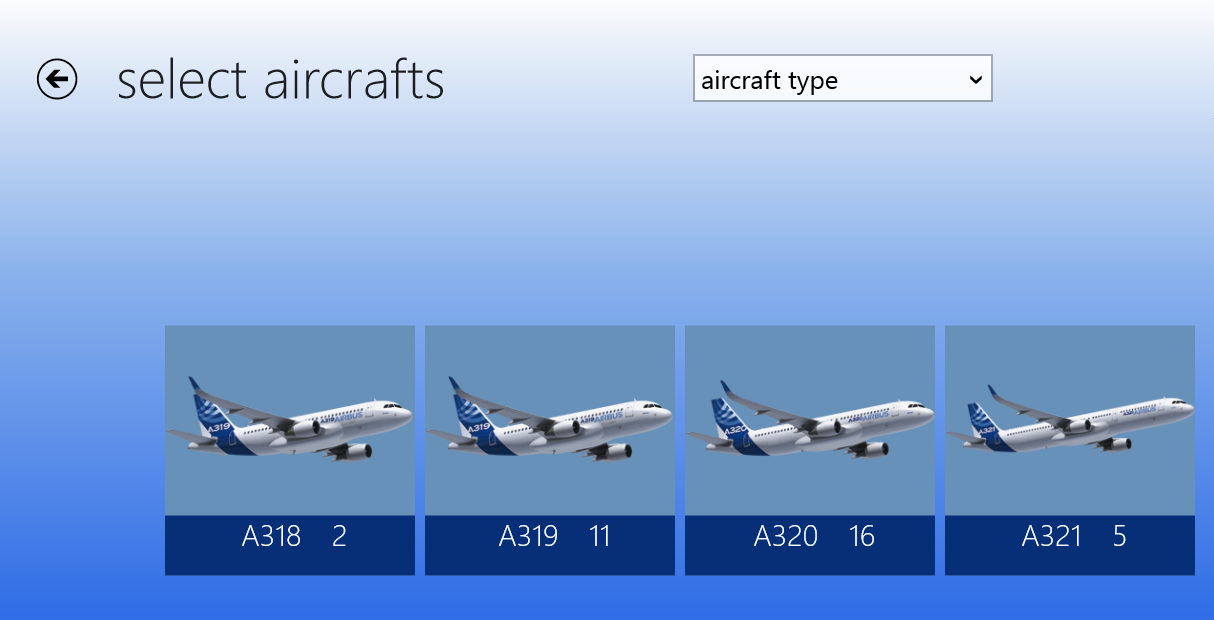
\includegraphics[width=\hsize]{images/impl/semantic_zoom_impl}
\caption{Herausgezoomte Ansicht der Flugzeugauswahl}
\label{aircraftSelectionZoomImpl}
\end{figure}

\subsection{Konfigurationsansicht}
Eine Übersicht der Konfigurationsergebnisse wird in der Zusammenfassungsseite (siehe \ref{configurationResultImpl}) gezeigt. Im Screenshot sind zwei Konfigurationsgruppen angezeigt, die beide komplett sind somit auch bestellt werden können. Der Abschluss der Konfiguration erfolgt mit den Buttons in der unteren AppBar. Die obere Leiste zeigt die Navigationsmöglichkeiten, die in der kompletten Anwendung vorhanden sind. Auf der rechten Seite können die Hauptansichten ausgewählt werden und auf der linken Seite kann zur Startseite navigiert werden. 
\begin{figure}[H]
\centering
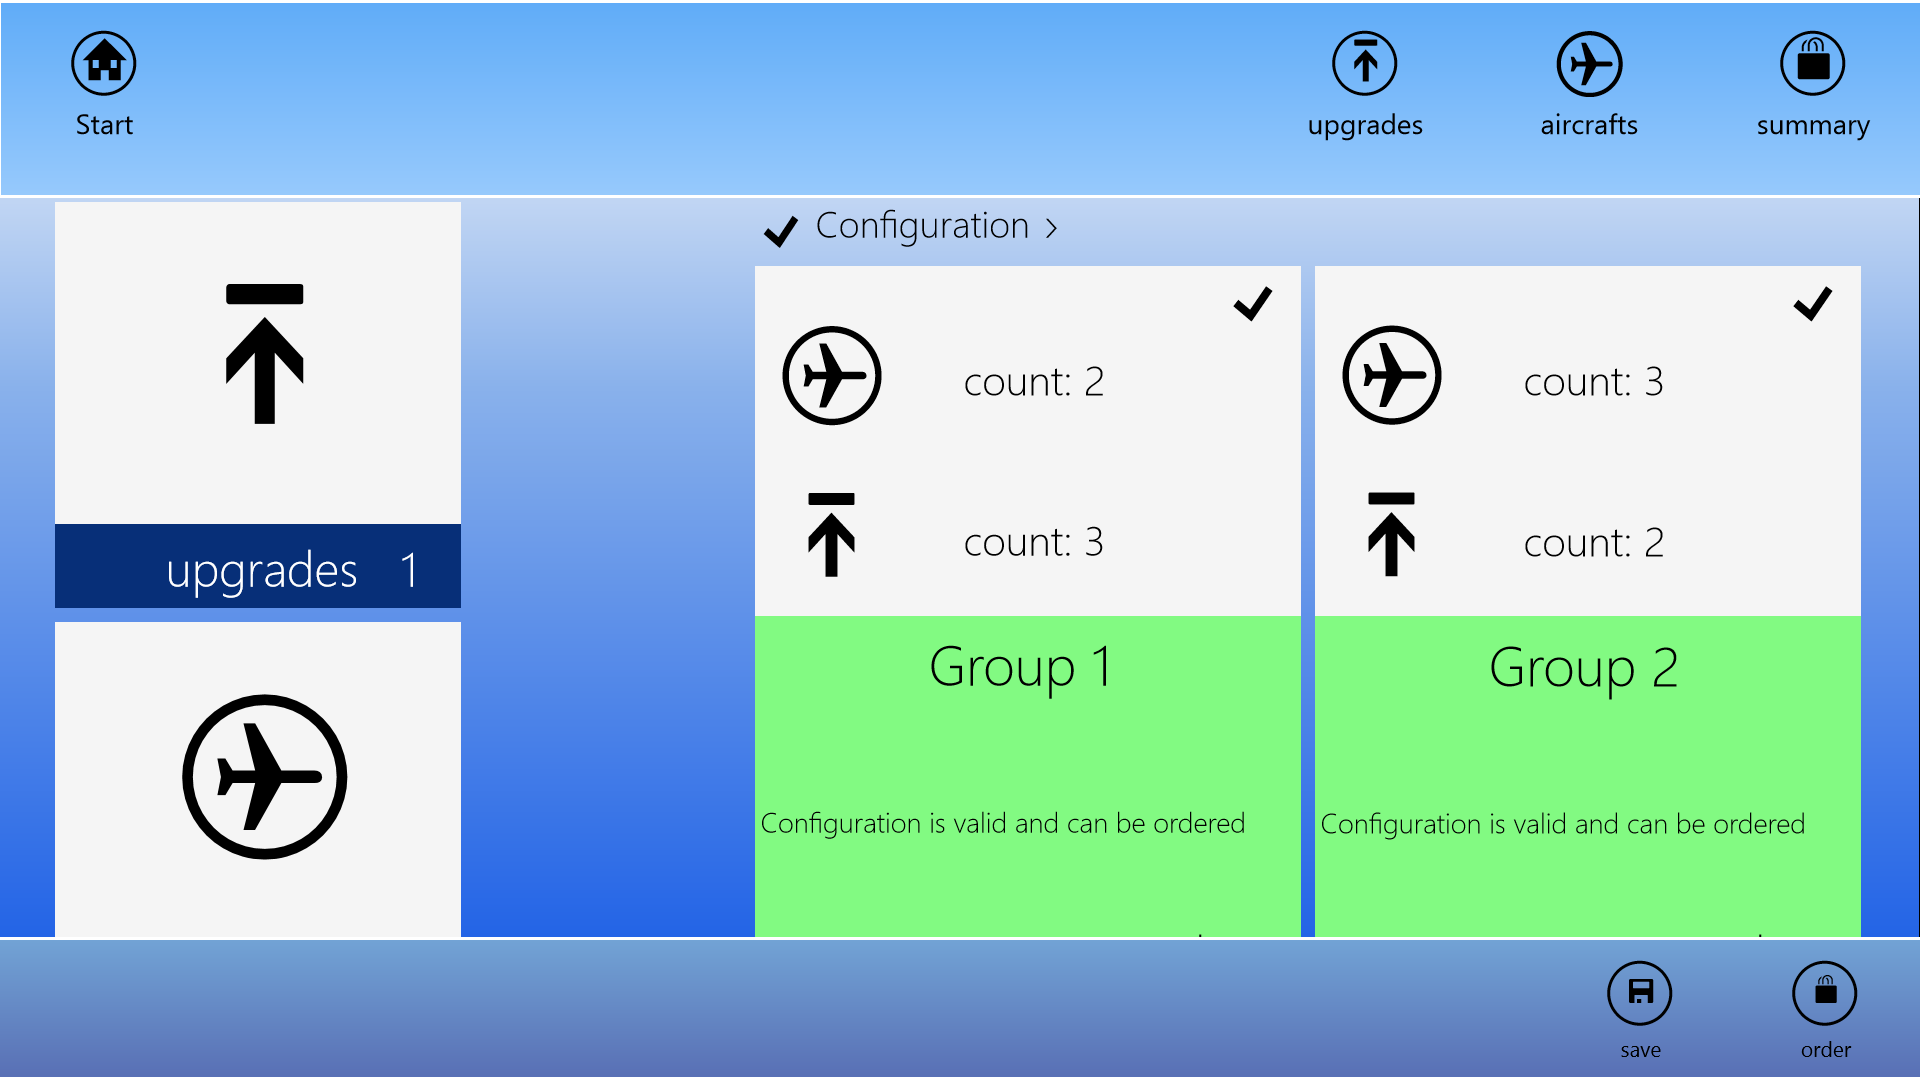
\includegraphics[width=\hsize]{images/impl/app_bar_impl}
\caption{Konfigurationsgruppen und Navigationsbar in der Zusammenfassung}
\label{configurationResultImpl}
\end{figure}
Die Auswahl der Alternativen ist in Abbildung \ref{alternativeSelectionImpl} dargestellt. Hier werden zuerst die bestimmten Alternativen angezeigt,die ausgewählt werden können. Zusätzlich sind die zuvor ausgewählten Upgrades vorhanden sowie die zur Konfigurationsgruppe gehörigen Flugzeuge. 
\begin{figure}[H]
\centering
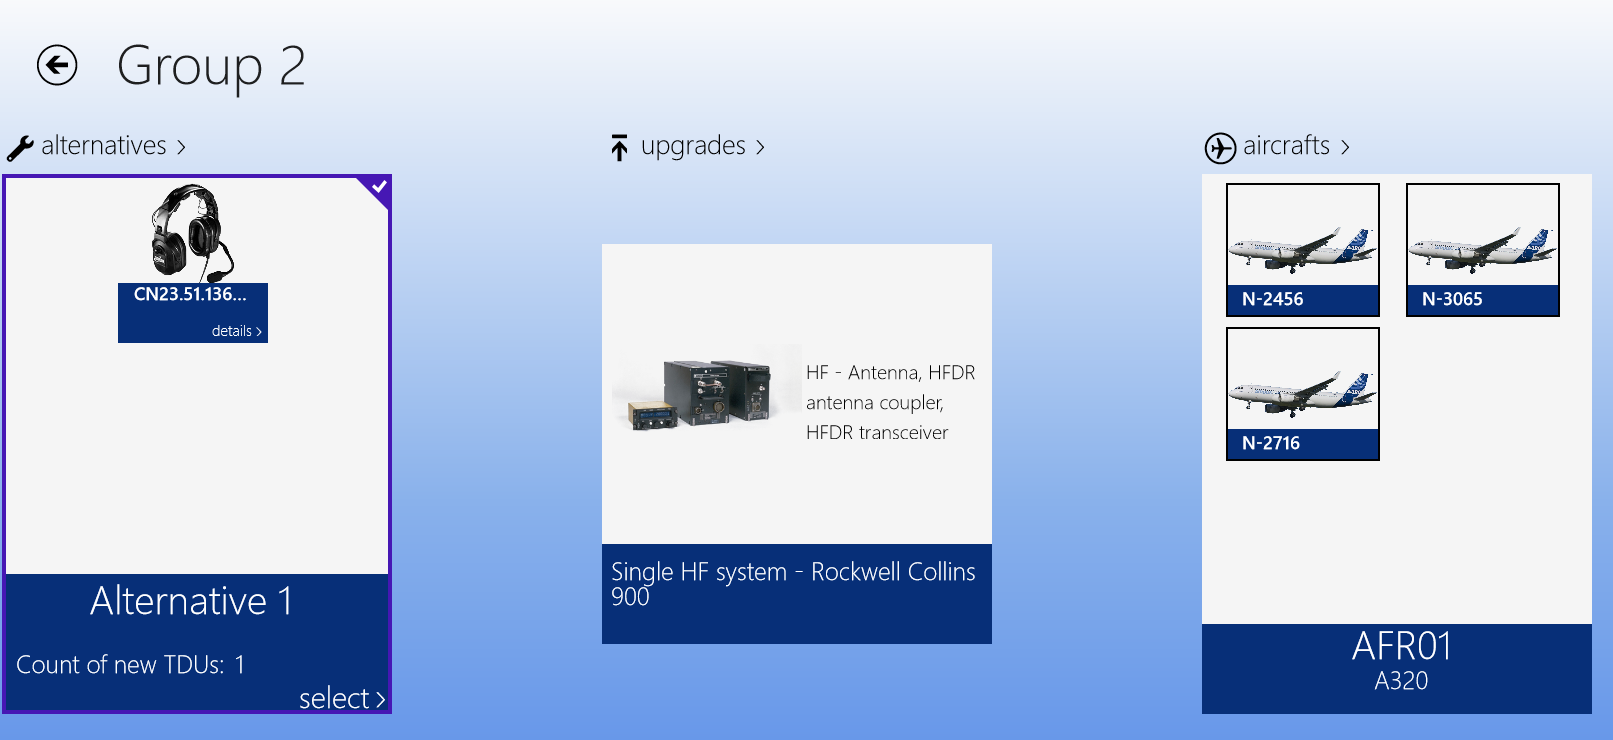
\includegraphics[width=\hsize]{images/impl/alternative_impl}
\caption{Alternativenauswahl für die zweite Konfigurationsgruppe}
\label{alternativeSelectionImpl}
\end{figure}

 
	\chapter{Evaluation der Anwendung}\label{chapter_6}
Damit ein Kunde einen besseren Einblick in das Produkt erhält, muss der Konfigurationsprozess vereinfacht werden. Die Vereinfachung des Prozesses wird ebenfalls durch eine einfache Bedienung der Anwendung erreicht. Die Sicherstellung, dass dieses Ziel bei der Entwicklung der App erreicht wurde, soll anhand einer heuristischen Evaluation herausgefunden werden. Hierbei wird eine bestimmte Anzahl an Benutzern herausgesucht, die eine Untersuchung der Anwendung durchführen. Die Heuristiken der einzelnen Benutzer ergeben sich aus bekannten Benutzungsprinzipien (siehe: \cite{bib:heuristik1}). Die Ergebnisse der Evaluation werden anhand der 10 Heuristiken von Nielsen \cite{bib:heuristik2} ausgewertet.


\section{Durchführung der Evaluation}
Für die Umstellung des Prozesses, wie in Kapitel \ref{chapter_3} beschrieben muss die Anwendung den neuen Prozess unterstützten. Hier muss die Evaluation die Frage beantworten, ob die Produktauswahl, sowie der Konfigurationsprozess verständlich ist. Damit ein Unterschied festgestellt werden kann, werden bestimmte Aufgaben der Anwendung zuerst auf der alten Konfigurationsoberfläche durchgeführt und anschließend mit der neuen Anwendung. Die Durchführung erfolgt hierbei in einer Interview Form, bei der eine Hilfestellung bei der Bedienung gegeben wird. Anschließend erhält der Anwender einen Fragebogen, der im Anhang zu finden ist. Mit diesem Vorgang erhält man zwei Rückmeldungen. Die Erste durch die verschiedenen Fragen der Benutzer bei der Anwendung und die zweite durch den ausgefüllten Fragebogen. Für eine aussagekräftige Evaluation wurden 4 Testpersonen ausgewählt. Zusätzlich zu der Benutzerevaluation wird eine zweite Evaluation der Experten durchgeführt. Hier wurde anhand der 10 Heuristiken ein Fragebogen angefertigt, der alle Merkmale enthält. Der Experte soll durch beliebiges Verwenden der Anwendung die Fragen bewerten. 


\section{Ergebnisse}

\subsection{Allgemeine Auswertung}
\subsection{Benutzerauswertung}
\subsection{Expertenauswertung}

	\chapter{Fazit und Ausblick}\label{chapter_7}
Bei der vorliegenden Arbeit wurde ein Weg gezeigt, wie ein komplexes Produkt anschaulich dargestellt werden kann. Das Aufbereiten der zugrundeliegenden Komplexität wurde durch eine anschauliche Umsetzung der Inhalte in einer mobilen, touchgesteuerten Umgebung erreicht. Durch diese Voraussetzung kann eine Vereinfachung des Konfigurationsprozesses mit einem Produktkonfigurator erfolgen. Innerhalb der Arbeit wurde eine Verbindung zwischen dem Produktkatalog und dem Konfigurator zu einer gemeinsamen Lösung erreicht.  Durch die Software aus einer Hand können die Geschäftsprozesse für eine Individualisierung des Produktes schneller durchgeführt werden und der Kunde erhält ein schnelleres Feedback zu seiner Auswahl. \par 

Beim Entwurf der Arbeit wurden die Besonderheiten der mobilen Zielumgebung genauso berücksichtigt, wie die Vorgaben der verwendeten Technologie. Hierdurch wurde eine auf die mobile Umgebung angepasste Anwendung entwickelt, die bei der anschließenden Evaluation überzeugen konnte. Die Auswertung der Fragebögen hat Probleme bei der Anwendung erkannt, die durch einen neuen Entwurf und Umsetzung der betroffenen Seite gelöst werden konnten. Bei der Implementierung konnte durch die Verwendung eines passenden Entwurfsmusters eine zukünftige Weiterentwicklung der App ermöglicht werden. Die Umsetzung des neuen Workflows wird sich beim Einsatz der Lösung bei einem Kunden zeigen. 
	%\chapter{Fazit und Ausblick}\label{chapter_8}

	\begin{appendix}
		\chapter{Anhang}


\section{Klassendiagramm}
\begin{figure}
\begin{lstlisting}
/// <summary>
    /// This View Model has the logic for aircraft family selection. Normally its the first view if
    /// a new configuration is started.
    /// </summary>
    public class SelectAircraftFamilyViewModel : GridHolderViewModel
    {
        private AircraftModel _model;
        private ICommand _familySelectedCommand;

        public SelectAircraftFamilyViewModel()
        {
            _model = new AircraftModel();
            InitializeDataSource();
        }

        private void InitializeDataSource()
        {

            DataGroupElements = new ObservableCollection<DataCommon>
                {new AircraftProgrammGroup(_model.GetAllAircraftProgramms())}; 
        }
\end{lstlisting} 
\begin{lstlisting}
        public ICommand SelectAircraftCommand
        {
            get { return _familySelectedCommand ?? (_familySelectedCommand = new RelayCommand<DataCommon>(SaveSelectionAndNavigateToSummaryPage)); }
            set
            {
                _familySelectedCommand = value;
                OnPropertyChanged();
            }
        }

        private void SaveSelectionAndNavigateToSummaryPage(DataCommon data)
        {
            var selectedProgramm = GetSelectedProgramm(data.UniqueId);
            _model.SelectAircraftProgramm(selectedProgramm);
            var classToNavigate = SimpleIoc.Default.GetInstance<ISummary>();
            var navigationService = SimpleIoc.Default.GetInstance<INavigationService>();
            navigationService.Navigate(classToNavigate.GetType());
        }

        private AircraftProgramm GetSelectedProgramm(string uniqueId)
        {
            return _model.GetAllAircraftProgramms().FirstOrDefault(programm => programm.UniqueId.Equals(uniqueId));
        }
    }
\end{lstlisting} 
\label{aircraftFamilySelectionViewModel}
\end{figure}
 
\section{Evaluationsergebnisse} \label{anhangEva}
	\end{appendix}
	
	% Anhang
	\clearpage
	\pagenumbering{roman}

	% Abbildungsverzeichnis
	\listoffigures
	\addcontentsline{toc}{chapter}{Abbildungsverzeichnis}
	
	\listoftables
	\addcontentsline{toc}{chapter}{Tabellenverzeichnis}
	
	
	% Literaturverzeichnis
	\clearpage
	\phantomsection
	\addcontentsline{toc}{chapter}{Literaturverzeichnis}
	\begin{thebibliography}{---}
\bibitem[MASS]{bib:massCustomization}
             \textsc{B. Joseph Pine}
            \textbf{Harvard Business Press}
            Mass customization, 1.Auflage , 1993
\bibitem[APP]{bib:businessApps}
             \textsc{Stephan Verclas, Claudia Linnhoff-Popien}
            \textbf{Springerverlag}
            Smart Mobile Apps: Mit Business-Apps ins Zeitalter mobiler Geschäftsprozesse, 1.Auflage , Dezember 2011
\bibitem[DESIGN]{bib:businessAppsDesign}
             \textsc{Christian Kraus}
            \textbf{2kit consulting}
            Grundlagen und Erfolgsfaktoren 
            für Apps im Mobile Business, Whitepaper , 16.05.2012

 \bibitem[PRODUCT]{bib:product}
            \textbf{Wirtschaftslexikon}
            Produkt, http://www.wirtschaftslexikon24.com/d/produkt/produkt.htm, aufgerufen am 25.07.2013
            
 \bibitem[BOOL1]{bib:boolescheAlgebra1}
 			\textsc{Helmut Herold, Bruno Lurz, Jürgen Wohlrab}
             \textbf{Pearson Studium}
             Grundlagen der Informatik, München 2006
             
 \bibitem[BOOL2]{bib:boolescheAlgebra2}
  			\textsc{Gerald Teschl, Susanne Teschl}
              \textbf{examen.press}
              Mathematik
              für Informatiker, Pearson Studium, Wien 2009, 3. Auflage
              
 
              			 
 \bibitem[PUPPE]{bib:puppe}
 			 \textsc{Frank Puppe}
 			 \textbf{Springerverlag}
 			 Einführung in Expertensysteme, 1. Auflag, 1988
 			 
 \bibitem[KELLER]{bib:keller}
  			 \textsc{Hubert B. Keller}
  			 \textbf{DH Karlsruhe}
  			 Wissensbasierte Systeme - Einführung, Vorlesung SS 2007
  			 
\bibitem[EXPERT]{bib:expert1}
			\textsc{Gerald Reif}
            \textbf{Deutsches Forschungszentrum für Knstliche Intelligenz}
            Expertensysteme, http://www.dfki.uni-kl.de/~aabecker/Mosbach/Experten/Reif-node8.html, aufgerufen am 18.07.2013
 
  \bibitem[TABLET]{bib:tableVertrieb}
            \textsc{Haufe}
           Tablets setzen sich durch, http://www.haufe.de/marketing-vertrieb/vertrieb/vertrieb-tablets-setzen-sich-durch\_130\_155918.html, aufgerufen am 26.07.2013           
            
 \bibitem[MOBILE1]{bib:mobileMarketing}
   			\textsc{Hans H. Bauer, Thorsten Dirks, Melchior D. Byant}
               \textbf{examen.press}
               Erfolgsfaktoren des mobile Marketing, Springer, 2008
               
 \bibitem[MOBILE2]{bib:mobileMarketing2}
                 \textbf{Pierre Audoin Consultants}
                 Tablets im Unternehmenseinsatz,http://www.berlecon.de/studien/downloads/PAC\_Trendstudie\_Microsoft\_Mobility\_May\_11.pdf,  Mai 2011
 
             
            
  \bibitem[RCP]{bib:eclipseRCP}
               \textsc{Ralf Ebert}
              Eclipse RCP, http://www.ralfebert.de/eclipse\_rcp/EclipseRCP.pdf, Version 1.1, 19.08.2011
  			
 			
\bibitem[ERGO]{bib:softwareErgonomie}
           \textsc{Christiane Rudlof}
          \textbf{Unfallkasse Post und Telekom}
          Handbuch Software-Ergonomie. Usebility Engineering., http://www.ukpt.de/pages/dateien/software-ergonomie.pdf, S.52, 2. Auflage, Tübingen 2006

 \bibitem[PLATTFORM]{bib:mobilePlattform}
           \textsc{Cloudsherpas}
          Native, Hybrid and Mobile Web Apps, http://www.cloudsherpas.com/services/custom-development/mobile-apps/native-hybrid-and-mobile-web-application-development/, aufgerufen am 23.07.2013

\bibitem[NATIVE]{bib:nativeBS}
           \textsc{statista}
          Apple bleibt Marktführer, http://de.statista.com/themen/580/tablets/infografik/758/prognose-der-weltweiten-marktanteile-der-tablet-betriebssysteme/, aufgerufen am 23.07.2013
          
\bibitem[PLATTFORM2]{bib:nativeBS2}
           \textsc{smartdigits}
          Native App oder Webb App, http://www.smart-digits.com/2012/02/native-app-oder-web-app-teil-1-definitionen-und-entscheidungskriterien/, aufgerufen am 23.07.2013
          
\bibitem[WEBAPP1]{bib:webappSafety}
           \textsc{Bundesamt für Sicherheit in der Informationstechnik}
           \textbf{SecureNet}
          Sicherheit von Webanwendungen, https://www.bsi.bund.de/SharedDocs/Downloads/DE/BSI/Publikationen/Studien/WebSec/WebSec\_pdf.pdf?\_blob=publicationFile, 1. Version, August 2006

\bibitem[WEBAPP2]{bib:webapp}
           \textsc{Andreas Schaffry}
           \textbf{CIO}
          Die Zukunft mobiler Anwendungen, http://www.cio.de/strategien/2910477/index.html  , aufgerufen am 27.07.2013

 \bibitem[WIN8-1]{bib:win81}
           \textsc{Bart Claeys, Qixing Zheng}
          \textbf{MSDN}
          Designfallstudie: vom iPad zur Windows Store-App, http://msdn.microsoft.com/de-de/library/windows/apps/hh868262, aufgerufen am 16.05.2013
          
  \bibitem[WIN8-2]{bib:win82}
            \textsc{Microsoft}
           \textbf{MSDN}
           Entwerfen großartiger Produktivitäts-Apps für Windows, http://msdn.microsoft.com/de-de/library/windows/apps/hh868273, aufgerufen am 16.05.2013
           
   \bibitem[WIN8-3]{bib:win83}
              \textsc{Microsoft}
             \textbf{MSDN}
             Shopping-Apps, http://msdn.microsoft.com/de-de/library/windows/apps/jj635241.aspx, aufgerufen am 16.05.2013
             
     \bibitem[WIN8-4]{bib:win84}
                \textsc{Microsoft}
               \textbf{MSDN}
 Planen ihrer App, http://msdn.microsoft.com/de-de/library/windows/apps/hh465427, aufgerufen am 16.05.2013

 
\end{thebibliography}


	
	% Abkürzungsverzeichnis
	% vorher in Konsole folgendes aufrufen: 
	%	makeglossaries makeglossaries dokumentation.acn && makeglossaries dokumentation.glo
	\printglossary[type=\acronymtype]
	
	% Glossar
	\printglossary[style=altlist,title=Glossar]
	
	
\end{document}

